% vim: set tw=80:spell
%
\documentclass[twoside,a5paper,10pt]{extarticle}
%\documentclass[twoside,14pt,draft]{extarticle}
%\documentclass[twoside,14pt,draft]{scrartcl}
\usepackage{amsmath}
\usepackage{amssymb}
\usepackage{amsfonts}
\usepackage{mathtext}
\usepackage{pdfpages}
\usepackage{parallel}
\usepackage[T2A]{fontenc}
\usepackage{ucs}
\usepackage[utf8x]{inputenc}
\usepackage[polish,english,russian]{babel}
\usepackage{hyperref}
\usepackage{rotating}
\usepackage[inner=2cm,top=1.8cm,outer=2cm,bottom=2.3cm,nohead]{geometry}
\usepackage{listings}
\usepackage{graphicx}
\usepackage{wrapfig}
\usepackage{longtable}
\usepackage{indentfirst}
\usepackage{array}
\newcolumntype{P}[1]{>{\raggedright\arraybackslash}p{#1}}
\frenchspacing
\usepackage{fixltx2e} %text sub- and superscripts
\usepackage{icomma} % коскі ў матэматычным рэжыме
\PreloadUnicodePage{4}

\newcommand{\longpage}{\enlargethispage{\baselineskip}}
\newcommand{\shortpage}{\enlargethispage{-\baselineskip}}

\def\switchlang#1{\expandafter\csname switchlang#1\endcsname}
\def\switchlangbe{
\let\saverefname=\refname%
\def\refname{Літаратура}%
\def\figurename{Іл.}%
}
\def\switchlangen{
\let\saverefname=\refname%
\def\refname{References}%
\def\figurename{Fig.}%
}
\def\switchlangru{
\let\saverefname=\refname%
\let\savefigurename=\figurename%
\def\refname{Литература}%
\def\figurename{Рис.}%
}

\hyphenation{admi-ni-stra-tive}
\hyphenation{ex-pe-ri-ence}
\hyphenation{fle-xi-bi-li-ty}
\hyphenation{Py-thon}
\hyphenation{ma-the-ma-ti-cal}
\hyphenation{re-ported}
\hyphenation{imp-le-menta-tions}
\hyphenation{pro-vides}
\hyphenation{en-gi-neering}
\hyphenation{com-pa-ti-bi-li-ty}
\hyphenation{im-pos-sible}
\hyphenation{desk-top}
\hyphenation{elec-tro-nic}
\hyphenation{com-pa-ny}
\hyphenation{de-ve-lop-ment}
\hyphenation{de-ve-loping}
\hyphenation{de-ve-lop}
\hyphenation{da-ta-ba-se}
\hyphenation{plat-forms}
\hyphenation{or-ga-ni-za-tion}
\hyphenation{pro-gramming}
\hyphenation{in-stru-ments}
\hyphenation{Li-nux}
\hyphenation{sour-ce}
\hyphenation{en-vi-ron-ment}
\hyphenation{Te-le-pathy}
\hyphenation{Li-nux-ov-ka}
\hyphenation{Open-BSD}
\hyphenation{Free-BSD}
\hyphenation{men-ti-on-ed}
\hyphenation{app-li-ca-tion}

\def\progref!#1!{\texttt{#1}}
\renewcommand{\arraystretch}{2} %Іначай формулы ў матрыцы зліпаюцца з лініямі
\usepackage{array}

\def\interview #1 (#2), #3, #4, #5\par{

\section[#1, #3, #4]{#1 -- #3, #4}
\def\qname{LVEE}
\def\aname{#1}
\def\q ##1\par{{\noindent \bf \qname: ##1 }\par}
\def\a{{\noindent \bf \aname: } \def\qname{L}\def\aname{#2}}
}

\def\interview* #1 (#2), #3, #4, #5\par{

\section*{#1\\{\small\rm #3, #4. #5}}

\def\qname{LVEE}
\def\aname{#1}
\def\q ##1\par{{\noindent \bf \qname: ##1 }\par}
\def\a{{\noindent \bf \aname: } \def\qname{L}\def\aname{#2}}
}

%\usepackage{portland}
%\usepackage{lscape}
%\usepackage{rotating}
\usepackage[labelsep=period,justification=centering]{caption}
%\usepackage{ccaption}
%\captiondelim{. }
\usepackage{tweaklist}
%\usepackage{trace}
%\usepackage{tikz}
%\usetikzlibrary{calc}
%\usetikzlibrary{positioning}
\usepackage{subfig}
\renewcommand{\enumhook}{\setlength{\topsep}{0pt}%
  \setlength{\itemsep}{0pt}\setlength{\parskip}{0pt plus 1pt minus 1pt}\setlength{\parsep}{0pt}}
\renewcommand{\itemhook}{\setlength{\topsep}{0pt}%
  \setlength{\itemsep}{0pt}\setlength{\parskip}{0pt plus 1pt minus 1pt}\setlength{\parsep}{0pt}}
%\renewcommand{\enumhook}{\setlength{\topsep}{0pt}%
%  \setlength{\itemsep}{0pt}}
%\renewcommand{\itemhook}{\setlength{\topsep}{0pt}%
%  \setlength{\itemsep}{0pt}\setlength{\parskip}{0pt}\setlength{\parsep}{0pt}}
%\renewcommand{\enumhook}{\setlength{\topsep}{0pt}%
%  \setlength{\itemsep}{0pt}}
%\renewcommand{\itemhook}{\setlength{\topsep}{0pt}%
%  \setlength{\itemsep}{0pt}\setlength{\parsep}{0pt}}

\clubpenalty=10000%
\widowpenalty=10000%
%\setlength{\parindent}{1.25cm}%

\newcommand\familyname[1]{\textbf{#1}}

\DeclareMathOperator{\e}{e}
\DeclareMathOperator{\cov}{cov}
\DeclareMathOperator{\diag}{diag}

\newcommand\eof{\writetotalpages\end{document}\endinput}

\newcommand\key[1]{\textbf{#1}}
\newcommand\vect[1]{\mathbf{#1}}
\def\eqn #1 $#2${\begin{equation}\label{eq:#1}#2\end{equation}}
%\def\where #1
\newcommand\eqnref[1]{(\ref{eq:#1})}
\makeatletter
\def\p@subfigure{\thefigure,~}
\def\thesubfigure{\asbuk{subfigure}}
\@newctr{figure}[section]
\renewcommand \thefigure {\@arabic\c@figure}
\@newctr{equation}[section]
\renewcommand\theequation{\@arabic\c@equation}
\newcommand\ps@twoside{%
 \makeatletter%
 \renewcommand\@oddfoot{~\hfill\thepage}%
 \renewcommand\@evenfoot{\thepage\hfill~}%
 \makeatother%
}
\newcounter{totalpages}
\def\writetotalpages{%
  \protected@write\@auxout
      {}%
      {\string\setcounter{totalpages}{\thepage}}}
\newcounter{totalfigures}%
\newcounter{totalsubfigures}%
\newcounter{totalsections}%
\newcounter{totalsubsections}%
\newcounter{totalsubsubsections}%
\newcounter{totalparagraphs}%

%\def\addcontentsline#1#2#3{%
%  \addtocontents{#1}{\protect\contentsline{#2}{#3}{\thepage}%
%  \protect\stepcounter{total#2s}}}
\makeatother
\newcommand\comment[1]{\textsf{#1}}
\renewcommand\labelitemi{\textendash}
\renewcommand\labelitemii{\textendash}


% перенос формул в тексте
\newcommand*{\hm}[1]{#1\nobreak\discretionary{}%
  {\hbox{$\mathsurround=0pt #1$}}{}}

\def\layersep{2.5cm}

\begin{document}
\addtocounter{page}{2}%
\pagestyle{twoside}

\thispagestyle{empty}
\newpage
\tableofcontents

\def\documentclass[#1]#2{}

\makeatletter

\def\@self@name{00}
\def\@preamble@name{preamble.tex}

\def\document{\newpage}
\let\@lvee@enddoc\enddocument

\let\@lvee@input\input
\def\enddocument{%
\gdef\@title{}%
\gdef\@author{}%
}

\newcounter{articleno}
\setcounter{articleno}0

\def\@lbibitem[#1]#2{\setlength{\topsep}{0pt}%
  \setlength{\itemsep}{0pt}\setlength{\parskip}{0pt plus 1pt minus 1pt}\setlength{\parsep}{0pt}%
    \item[\@biblabel{#1}\hfill]\if@filesw
      {\let\protect\noexpand
       \immediate
       \write\@auxout{\string\bibcite{#2}{#1}}}\fi\ignorespaces}
\def\@bibitem#1{\setlength{\topsep}{0pt}%
  \setlength{\itemsep}{0pt}\setlength{\parskip}{0pt plus 1pt minus 1pt}\setlength{\parsep}{0pt}%
    \item\if@filesw \immediate\write\@auxout
       {\string\bibcite{#1}{\the\value{\@listctr}}}\fi\ignorespaces}

\renewcommand\maketitle{\par
  \begingroup
     \def\@thanks{}% flush all the thanks we have already collected so they don't accumulate
     \renewcommand\thefootnote{\@fnsymbol\c@footnote}%
     \def\@makefnmark{\rlap{\@textsuperscript{\normalfont\@thefnmark}}}%
     \long\def\@makefntext##1{\parindent 1em\noindent
             \hb@xt@1.8em{%
                 \hss\@textsuperscript{\normalfont\@thefnmark}}##1}%
%     \if@twocolumn
%       \ifnum \col@number=\@ne
%         \@maketitle
%       \else
%         \twocolumn[\@maketitle]%
%       \fi
%     \else
      \newpage
      \global\@topnum\z@   % Prevents figures from going at top of page.
      \stepcounter{articleno}%
      \def\footnote##1{}
      \ifx \@author \@empty
          \addcontentsline{toc}{section}{\@title}%
      \else
          \addcontentsline{toc}{section}{\@author: \@title}%
      \fi
      \@maketitle
%     \fi
    \thispagestyle{twoside}\@thanks
  \endgroup
  \setcounter{footnote}{0}%
}

\def\@maketitle{%
  \newpage
  \null
  \vskip 1em%
  \begin{center}%
  \let \footnote \thanks
    {\LARGE \@title \par}%
    {\large
      \lineskip .2em%
      \begin{tabular}[t]{c}%
        \@author
      \end{tabular}\par}%
  \end{center}%
  \par
}

\def\input#1{
\def\@@@curfile{#1}
\message{@@\@@@curfile @@}
\ifx \@@@curfile \@preamble@name
    \message{An attempt to include the preamble has occured, ignoring.^^J}
\else
    \ifx \@@@curfile \@self@name
        \message{An attempt to include ourselves had occured, ignoring.^^J}
    \else
        \@lvee@input#1
    \fi
\fi
}

\def\abstract{%
        \small%
        \quotation \noindent}

\makeatother

\documentclass[10pt, a5paper]{article}
\usepackage{pdfpages}
\usepackage{parallel}
\usepackage[T2A]{fontenc}
\usepackage{ucs}
\usepackage[utf8x]{inputenc}
\usepackage[polish,english,russian]{babel}
\usepackage{hyperref}
\usepackage{rotating}
\usepackage[inner=2cm,top=1.8cm,outer=2cm,bottom=2.3cm,nohead]{geometry}
\usepackage{listings}
\usepackage{graphicx}
\usepackage{wrapfig}
\usepackage{longtable}
\usepackage{indentfirst}
\usepackage{array}
\newcolumntype{P}[1]{>{\raggedright\arraybackslash}p{#1}}
\frenchspacing
\usepackage{fixltx2e} %text sub- and superscripts
\usepackage{icomma} % коскі ў матэматычным рэжыме
\PreloadUnicodePage{4}

\newcommand{\longpage}{\enlargethispage{\baselineskip}}
\newcommand{\shortpage}{\enlargethispage{-\baselineskip}}

\def\switchlang#1{\expandafter\csname switchlang#1\endcsname}
\def\switchlangbe{
\let\saverefname=\refname%
\def\refname{Літаратура}%
\def\figurename{Іл.}%
}
\def\switchlangen{
\let\saverefname=\refname%
\def\refname{References}%
\def\figurename{Fig.}%
}
\def\switchlangru{
\let\saverefname=\refname%
\let\savefigurename=\figurename%
\def\refname{Литература}%
\def\figurename{Рис.}%
}

\hyphenation{admi-ni-stra-tive}
\hyphenation{ex-pe-ri-ence}
\hyphenation{fle-xi-bi-li-ty}
\hyphenation{Py-thon}
\hyphenation{ma-the-ma-ti-cal}
\hyphenation{re-ported}
\hyphenation{imp-le-menta-tions}
\hyphenation{pro-vides}
\hyphenation{en-gi-neering}
\hyphenation{com-pa-ti-bi-li-ty}
\hyphenation{im-pos-sible}
\hyphenation{desk-top}
\hyphenation{elec-tro-nic}
\hyphenation{com-pa-ny}
\hyphenation{de-ve-lop-ment}
\hyphenation{de-ve-loping}
\hyphenation{de-ve-lop}
\hyphenation{da-ta-ba-se}
\hyphenation{plat-forms}
\hyphenation{or-ga-ni-za-tion}
\hyphenation{pro-gramming}
\hyphenation{in-stru-ments}
\hyphenation{Li-nux}
\hyphenation{sour-ce}
\hyphenation{en-vi-ron-ment}
\hyphenation{Te-le-pathy}
\hyphenation{Li-nux-ov-ka}
\hyphenation{Open-BSD}
\hyphenation{Free-BSD}
\hyphenation{men-ti-on-ed}
\hyphenation{app-li-ca-tion}

\def\progref!#1!{\texttt{#1}}
\renewcommand{\arraystretch}{2} %Іначай формулы ў матрыцы зліпаюцца з лініямі
\usepackage{array}

\def\interview #1 (#2), #3, #4, #5\par{

\section[#1, #3, #4]{#1 -- #3, #4}
\def\qname{LVEE}
\def\aname{#1}
\def\q ##1\par{{\noindent \bf \qname: ##1 }\par}
\def\a{{\noindent \bf \aname: } \def\qname{L}\def\aname{#2}}
}

\def\interview* #1 (#2), #3, #4, #5\par{

\section*{#1\\{\small\rm #3, #4. #5}}

\def\qname{LVEE}
\def\aname{#1}
\def\q ##1\par{{\noindent \bf \qname: ##1 }\par}
\def\a{{\noindent \bf \aname: } \def\qname{L}\def\aname{#2}}
}


\begin{document}

\title{Cells.js --- еще один подход к разработке современных веб-приложений}

\author{Алексей Кондратенко\\
\small Altoros Development, \texttt{alk@tut.by}
}
\maketitle

\begin{abstract}
Membase NoSQL database management system has administrative interface 
implemented as modern ``single-page'' aka ``pure-js'' web application. 
This talk will describe Cells.js --- a library that was grown inside 
this user interface component. It facilitates structuring of user 
interface as a collection of inter-dependent variables or cells. This 
provides some otherwise hard to implement features, like back button 
support, for free. And I believe, that this leads to cleaner and smaller 
code base.
\end{abstract}

В последние годы получила распостранение такая практика организации
веб-приложений, когда на стороне браузера реализуется вся логика
пользователького интерфейса. Серверная сторона при этом предоставляет
только <<голый>> API для доступа к данным. Преимуществом такого подхода
является более отзывчивый интерфейс, т.к. реакция на действия
пользователя реализуется на стороне браузера.

Одной из проблем построения пользователького интерфейса в таком виде
является относительная неадаптированность современных web-стандартов
к такого рода приложениям. Эти стандарты создавались в основном для
статического web. Другой известной проблемой является неполная или
неправильная реализация стандартов в разных браузерах.

Для реализации несложной логики зачастую достаточно применить одну из
библиотек для кросс-браузерного манипулирования DOM и кросс-браузерной
реализации \verb!XMLHttpRequest!. В последнее время в этой нише доминирует
библиотека jquery. Реализация более сложной логики быстро превращает
код в запутанную и трудно поддерживаемую кашу из обработчиков событий и 
требует перехода к какому-либо способу организации более богатого
пользователького интерфейса.

К одному из таких способов относятся MVC и его производные. На
сегодняшний день имеется масса тяжеловесных фреймворков для
реализации MVC, например Google Web Toolkit, ExtJS, SproutCore.

Однако, на мой взгляд, в средних по размеру приложениях применение более
компактных и простых решений оправдано.

При создании web-интерфейса для Membase было изначально решено
использовать только jquery. Однако после реализации первых экранов я
понял, что без более продвинутой организации логики этот код будет
невозможно поддерживать и развивать.

Большинство MVC-фреймворков имеет в своем основании систему наблюдения
за данными и реакции на их изменения. Это позволяет отделять логику
получения/обработки данных от логики обработки пользователькой реакции
и логики представления этих данных пользователю.

Я начал с создания простого класса, реализующего наблюдаемое значение и
возможность <<подписаться>> на его измeнения. Это помогло
структурировать код лучше. Но затем я заметил, что некоторые значения
полностью детерминированно зависят от других значений. Я вспомнил про
проект cells, реализованный на common-lisp 
(\url{http://common-lisp.net/project/cells/}) и понял, что могу легко
реализовать основную идею этого проекта на javascript.

В результате пользователький интерфейс Membase (и до этого Northscale
Memcached Server) организован как набор связаных зависимостями по
данным ячеек. Большинство ячеек является вычисляемыми, т.е. каждой из
них соответствует детерминированная функция на javascript. Значения
функций вычисляемых ячеек могут зависеть только от значений других
ячеек. И библиотека организует (пере)вычисления ячеек когда значения
их зависимостей либо становится известно, либо изменяется.

Когда одной из исходных ячеек присваивается какое-либо значение,
например, в результате действия пользователя, cells.js организует
перевычисление всех ячеек, которые зависят от этой ячейки. После чего
перевычисляются ячейки, зависимые от только что перевычисленных ячеек, и
так далее. T.e. cells.js организует <<расплывание>> данных (и, в
некотором роде, реакции) по ячейкам.

Видимые пользователью блоки пользователького интерфейса подписываются
на значениe ячейки, которую отображают, и обновляются автоматически.

cells.js позволяет связывать hash-фрагменты URL с ячейками. Так что
кнопка <<назад>>, которая просто меняет URL страницы, работает
автоматически. При этом просто меняется значение одной из исходных
ячеек, и остальная часть пользователького интерфейса обновляется
соответственно.

cells.js реализует получение данных с сервера HTTP GET-запросом как
один из видов вычисления значения. Пока запрос загружается, значение
ячейки --- undefined. Зависимые от этой ячейки блоки интерфейса
обычно реагируют на это отображением индикатора загрузки. Это
поведение реализуется автоматически в коде связывания ячейки и
HTML-шаблона с блоком.

URL GET-запросов как правило берется из других ячеек. В результате
REST API Membase большей частью реально реализован через гипертекст
(что соответствует каноническому определению REST). Ссылки на GET-запросы 
берутся из ответов на другие запросы.

Изменение ячейки с URL побуждает зависимую ячейку с содержимым этого
URL выполнить запрос повторно с новым URL.

Так, например, реакция пользователя может поменять имя (или какой-либо
идентификатор) выделенного обьекта. Зависимая от имени ячейка может
находить URL этого обьекта по имени в <<листинге>> обьектов, который
содержит список пар имя--URL, и ячейка с описанием этого обьекта может
просто получать его GET-запросом с сервера. Смена выделенного имени
будет автоматически приводить к получению актуального описания
выделенного обьекта, и отображение этой ячейки будет также меняться
автоматически.

Считаю, что такой способ организации пользователького интерфейса
является очень логичным и продуктивным.  Он позволил в очень
короткие сроки реализовать довольно продвинутый web-интерфейс Membase.

На момент написания этого текста cells все еще является частью
Membase. Как и весь код Membase, код cells доступен по лицензии Apache
версии 2.0. В ближайшее время планирую закончить работу по вынесению
cells в отдельный независимый free-software проект.
\end{document}





\documentclass[10pt, a5paper]{article}
\usepackage{pdfpages}
\usepackage{parallel}
\usepackage[T2A]{fontenc}
\usepackage{ucs}
\usepackage[utf8x]{inputenc}
\usepackage[polish,english,russian]{babel}
\usepackage{hyperref}
\usepackage{rotating}
\usepackage[inner=2cm,top=1.8cm,outer=2cm,bottom=2.3cm,nohead]{geometry}
\usepackage{listings}
\usepackage{graphicx}
\usepackage{wrapfig}
\usepackage{longtable}
\usepackage{indentfirst}
\usepackage{array}
\newcolumntype{P}[1]{>{\raggedright\arraybackslash}p{#1}}
\frenchspacing
\usepackage{fixltx2e} %text sub- and superscripts
\usepackage{icomma} % коскі ў матэматычным рэжыме
\PreloadUnicodePage{4}

\newcommand{\longpage}{\enlargethispage{\baselineskip}}
\newcommand{\shortpage}{\enlargethispage{-\baselineskip}}

\def\switchlang#1{\expandafter\csname switchlang#1\endcsname}
\def\switchlangbe{
\let\saverefname=\refname%
\def\refname{Літаратура}%
\def\figurename{Іл.}%
}
\def\switchlangen{
\let\saverefname=\refname%
\def\refname{References}%
\def\figurename{Fig.}%
}
\def\switchlangru{
\let\saverefname=\refname%
\let\savefigurename=\figurename%
\def\refname{Литература}%
\def\figurename{Рис.}%
}

\hyphenation{admi-ni-stra-tive}
\hyphenation{ex-pe-ri-ence}
\hyphenation{fle-xi-bi-li-ty}
\hyphenation{Py-thon}
\hyphenation{ma-the-ma-ti-cal}
\hyphenation{re-ported}
\hyphenation{imp-le-menta-tions}
\hyphenation{pro-vides}
\hyphenation{en-gi-neering}
\hyphenation{com-pa-ti-bi-li-ty}
\hyphenation{im-pos-sible}
\hyphenation{desk-top}
\hyphenation{elec-tro-nic}
\hyphenation{com-pa-ny}
\hyphenation{de-ve-lop-ment}
\hyphenation{de-ve-loping}
\hyphenation{de-ve-lop}
\hyphenation{da-ta-ba-se}
\hyphenation{plat-forms}
\hyphenation{or-ga-ni-za-tion}
\hyphenation{pro-gramming}
\hyphenation{in-stru-ments}
\hyphenation{Li-nux}
\hyphenation{sour-ce}
\hyphenation{en-vi-ron-ment}
\hyphenation{Te-le-pathy}
\hyphenation{Li-nux-ov-ka}
\hyphenation{Open-BSD}
\hyphenation{Free-BSD}
\hyphenation{men-ti-on-ed}
\hyphenation{app-li-ca-tion}

\def\progref!#1!{\texttt{#1}}
\renewcommand{\arraystretch}{2} %Іначай формулы ў матрыцы зліпаюцца з лініямі
\usepackage{array}

\def\interview #1 (#2), #3, #4, #5\par{

\section[#1, #3, #4]{#1 -- #3, #4}
\def\qname{LVEE}
\def\aname{#1}
\def\q ##1\par{{\noindent \bf \qname: ##1 }\par}
\def\a{{\noindent \bf \aname: } \def\qname{L}\def\aname{#2}}
}

\def\interview* #1 (#2), #3, #4, #5\par{

\section*{#1\\{\small\rm #3, #4. #5}}

\def\qname{LVEE}
\def\aname{#1}
\def\q ##1\par{{\noindent \bf \qname: ##1 }\par}
\def\a{{\noindent \bf \aname: } \def\qname{L}\def\aname{#2}}
}


\begin{document}

\title{Организация программной защиты от DDoS-атак }

\author{Олег Бойцев\\
\small Минск, \texttt{[Mega-Admin.com][, infosecurity@ya.ru}
}
\maketitle

\begin{abstract}
DDoS Mitigation Software Solutions. The report outlines experience in deploying software protection against DDoS attacks using OS Linux. The following  issues of organization of DDoS attacks are reviewed: the psychology of the attackers, the tools and techniques they use. In the report of the conference participants will receive an answer to the question: Is it possible to defeat DDoS without hardware tools and if so, how?
\end{abstract}

\section*{Введение}
Тема DDoS/antiDDoS бесспорно является интересной и актуальной. 

Для многих компаний предоставление сервисов и услуг  online является чуть ли не единственной формой ведения бизнеса (\url{www.mastercard.com}, \url{www.facebook.com}, \url{www.habrahabr.ru}) в связи с чем, доступность сервиса онлайн можно считать критически важным условием успешного развития компании. Простой онлайн сервиса, даже на не продолжительное время, для компании может оказаться слишком дорогим <<удовольствием>>\ldots

\section*{Экономика DDoS-атак}
Как и в реальной экономике, расчет стоимости DDoS-атаки на сайт определяется прежде всего соотношением спрос/предложение. Цена также определяется и <<весом>> сайта "--- чем крупнее клиент, тем больше обычно просят за него.
Для примера: на момент написания тезисов доклада средняя стоимость ддос атаки на среднестатистический сайт составляла \$50. Приблизительно такова же и стоимость защиты в сутки. Стоимость покупки ботнета составляет \$1500--\$2000.

\section*{Какие DDoS-атаки бывают, какие из них используют чаще всего}
В зависимости от целей  чаще всего используют следующие типы атак:  
\begin{itemize}
\item HTTP flood,
\item TCP flood,
\item UDP/ICMP flood.
\end{itemize}

\section*{Инструменты для проведения DDoS-атак}
За последние годы инструменты проведения DDoS-атак значительно видоизменились. То, что раньше было доступно узкому кругу избранным, в настоящее время поставлено на поток. Общей  тенденцией развития инструментов проведения ддос атак можно считать: использование децентрализованной структуры управления \linebreak ботнетом, упрощение user-end интерфейсов управления, шифрование трафика боты "--- командный центр.

\section*{Модель многоуровневой защиты от DDoS-атак}
Firewall → Linux kernel → scripts → nginx → apache
\begin{itemize}
\item Firewall: ограничиваем количество соединений в единицу времени, режем ботов через  string module
\item Linux kernel: уменьшаем таймауты на обработку соединений, повышаем лимит общего количества возможных соединений, предел используемой памяти.
\item Scripts: режем сетевые аномалии
\item Nginx: тюнингуем, прикручиваем  limit\_conn
\item Apache: тюнингуем, прикручиваем mod-evasive
\end{itemize}

\section*{Что можно победить}
Все что не толще ширины канала сервера.

В случае если толщина DDoS-атаки больше ширина канала "--- железно фильтруем трафик на входе в ДЦ.
\end{document}





\documentclass[a4paper,12pt]{article}

\usepackage{pdfpages}
\usepackage{parallel}
\usepackage[T2A]{fontenc}
\usepackage{ucs}
\usepackage[utf8x]{inputenc}
\usepackage[polish,english,russian]{babel}
\usepackage{hyperref}
\usepackage{rotating}
\usepackage[inner=2cm,top=1.8cm,outer=2cm,bottom=2.3cm,nohead]{geometry}
\usepackage{listings}
\usepackage{graphicx}
\usepackage{wrapfig}
\usepackage{longtable}
\usepackage{indentfirst}
\usepackage{array}
\newcolumntype{P}[1]{>{\raggedright\arraybackslash}p{#1}}
\frenchspacing
\usepackage{fixltx2e} %text sub- and superscripts
\usepackage{icomma} % коскі ў матэматычным рэжыме
\PreloadUnicodePage{4}

\newcommand{\longpage}{\enlargethispage{\baselineskip}}
\newcommand{\shortpage}{\enlargethispage{-\baselineskip}}

\def\switchlang#1{\expandafter\csname switchlang#1\endcsname}
\def\switchlangbe{
\let\saverefname=\refname%
\def\refname{Літаратура}%
\def\figurename{Іл.}%
}
\def\switchlangen{
\let\saverefname=\refname%
\def\refname{References}%
\def\figurename{Fig.}%
}
\def\switchlangru{
\let\saverefname=\refname%
\let\savefigurename=\figurename%
\def\refname{Литература}%
\def\figurename{Рис.}%
}

\hyphenation{admi-ni-stra-tive}
\hyphenation{ex-pe-ri-ence}
\hyphenation{fle-xi-bi-li-ty}
\hyphenation{Py-thon}
\hyphenation{ma-the-ma-ti-cal}
\hyphenation{re-ported}
\hyphenation{imp-le-menta-tions}
\hyphenation{pro-vides}
\hyphenation{en-gi-neering}
\hyphenation{com-pa-ti-bi-li-ty}
\hyphenation{im-pos-sible}
\hyphenation{desk-top}
\hyphenation{elec-tro-nic}
\hyphenation{com-pa-ny}
\hyphenation{de-ve-lop-ment}
\hyphenation{de-ve-loping}
\hyphenation{de-ve-lop}
\hyphenation{da-ta-ba-se}
\hyphenation{plat-forms}
\hyphenation{or-ga-ni-za-tion}
\hyphenation{pro-gramming}
\hyphenation{in-stru-ments}
\hyphenation{Li-nux}
\hyphenation{sour-ce}
\hyphenation{en-vi-ron-ment}
\hyphenation{Te-le-pathy}
\hyphenation{Li-nux-ov-ka}
\hyphenation{Open-BSD}
\hyphenation{Free-BSD}
\hyphenation{men-ti-on-ed}
\hyphenation{app-li-ca-tion}

\def\progref!#1!{\texttt{#1}}
\renewcommand{\arraystretch}{2} %Іначай формулы ў матрыцы зліпаюцца з лініямі
\usepackage{array}

\def\interview #1 (#2), #3, #4, #5\par{

\section[#1, #3, #4]{#1 -- #3, #4}
\def\qname{LVEE}
\def\aname{#1}
\def\q ##1\par{{\noindent \bf \qname: ##1 }\par}
\def\a{{\noindent \bf \aname: } \def\qname{L}\def\aname{#2}}
}

\def\interview* #1 (#2), #3, #4, #5\par{

\section*{#1\\{\small\rm #3, #4. #5}}

\def\qname{LVEE}
\def\aname{#1}
\def\q ##1\par{{\noindent \bf \qname: ##1 }\par}
\def\a{{\noindent \bf \aname: } \def\qname{L}\def\aname{#2}}
}


\renewcommand{\arraystretch}{2} %Іначай формулы ў матрыцы зліпаюцца з лініямі

% To be edited when needed %%%%%%%%%%
\newcommand{\progname}{\textit} % Стыль адлюстравання імёнаў праграм
\newcommand{\aknowl}{\textit} % Стыль для падзяк
%%%%%%%%%%%%%%%%%%%%%%%%%%%%%%%%%%%%%

\begin{document}

\renewcommand{\figurename}{Рыс.} % Не перакідаць у прэамбулу --- не працуе, чаму -- халера ведае.
\renewcommand{\abstractname}{Анатацыя}
\renewcommand{\refname}{Літаратура}

\title{Шляхі акселерацыі выканання вылічальнай нагрузкі на Python}
\author{Антон Літвіненка\\ \small Кіеўскі нацыянальны ўніверсітэт імя Тараса Шаўчэнкі\\ \small \texttt{tenebrosus.scriptor@gmail.com}}
\date{}
\maketitle

\begin{abstract}
Interpreted programming languages are known for their flexibility and convenience, but suffer from low execution speed comparing to compiled ones. However, they find a use for time-consuming applications. The enhanced methods of acceleration for interpreted languages are available, first of all just-in-time (JIT) compilation. The effect of the JIT compilation on the execution speed of a time-consuming scientific program is reported, and a few implementations of JIT compilers for Python are compared. \progname{PyPy} was found to be the fastest one, \progname{Psyco} --- slightly slower, \progname{Unladen Swallow} --- nearly useless.
\end{abstract}

Інтэрпрэтаваныя мовы праграмавання ўсё часцей ужываюцца пры напісанні ПЗ для разнастайных сфераў дастасавання, у тым ліку такіх, што традыцыйна не асацыююцца з інтэрпрэтаванымі мовамі, а менавіта --- напісанне ПЗ, якое патрабуе вялікіх вылічальных рэсурсаў.

Так, напрыклад, існуе часткова напісаная на Python бібліятэка для квантавахімічнага мадэліравання \progname{pDynamo} \cite{pDynamo}, аўтары якой адмовіліся ад традыцыйнага ў гэтай галіне выбару між Fortran, C або C++ і сваіх ранейшых напрацовак на Fortran, і аддалі перавагу інтэрфейсу на Python (з рэалізацыяй найбольш крытычнай да хуткасці часткі коду на C). Прычыны поспехаў інтэрпрэтаваных моў у гэтай галіне ў выпадку навуковых праграм, верагодна, абумоўленыя лёгкасцю распрацоўкі для неадмыслоўцаў.

Таксама гэтыя мовы зручнейшыя для распрацоўкі з элементамі рэфлектыўнага праграмавання (а менавіта, калі праграме неабходна генераваць частку ўласнага коду).

Аўтарам дакладу была распрацаваная праграма \progname{Mj{\"o}llnir}, якая выконвае інтэрпрэтацыю вынікаў магнетахімічнага эксперыменту з выкарыстаннем паўнаматрычнага метаду рашэння аператарных ураўненняў для спін-гамільтаніяна магнітных узаемадзеянняў, зыходзячы з мадэлі, якая задаецца карыстальнікам \cite{Mjollnir}. Для рашэння гэтае задачы неабходна на падставе мадэлі пабудаваць матрыцы спін-гамільтаніяна (прыклад на рыс.~\ref{fig:spin_ham}), прычым у алгебраічным (сімвальным) выглядзе. Алгарытм пабудовы быў рэалізаваны на Python. Праграму можна атрымаць ад аўтара пад умовамі ліцэнзіі GNU GPL v3.

Безумоўна, праблема хуткасці выканання ў такім выпадку становіцца актуальнай.


\begin{figure}[ht]
$$
\left(
\begin{array}{c|cccc}
\mathit{z}&|+\frac{1}{2};+\frac{1}{2}\rangle&|+\frac{1}{2};-\frac{1}{2}\rangle&|-\frac{1}{2};+\frac{1}{2}\rangle&|-\frac{1}{2};-\frac{1}{2}\rangle\\
\hline
\langle+\frac{1}{2};+\frac{1}{2}|&\mu H_zg_z-\frac{1}{2}J_z&0&0&0\\
\langle+\frac{1}{2};-\frac{1}{2}|&0&\frac{1}{2}J_z&-J_z&0\\
\langle-\frac{1}{2};+\frac{1}{2}|&0&-J_z&\frac{1}{2}J_z&0\\
\langle-\frac{1}{2};-\frac{1}{2}|&0&0&0&-\mu H_zg_z-\frac{1}{2}J_z\\
\end{array}
\right)
$$
\caption{Матрыца спін-гамільтаніяна для асі \textit{z} для комплексу Cu\textsubscript{2}.}
\label{fig:spin_ham}
\end{figure}

Метады акселерацыі выканання прадугледжваюць адыход ад чыстай інтэрпрэтацыі зыходнага коду ў момант выканання і пераход да разнастайных гібрыдных схемаў трансляцыі.

Па-першае, самая крытычная да рэсурсаў частка функцыянальнасці можа быць напісаная на кампіляванай мове праграмавання. Але такі падыход патрабуе перапісвання коду і можа ўскладняць рэалізацыю.

Ускосным дастасаваннем такога падыходу з'яўляецца выкарыстанне адных канструкцый мовы замест іншых, аналагічных, але хутчэйшых\cite{Optimize}.  Так, сапраўды, інструкцыя:
\begin{lstlisting}
    map(operator.add, l1, l2) 
\end{lstlisting}
хутчэй, чым:
\begin{lstlisting}
    map(lambda x,y: x+y, l1, l2)
\end{lstlisting}
 А спроба сабраць матрыцу ў адзін радок інструкцыяй:
\begin{lstlisting}
    collect_str+=a[i][j]  
\end{lstlisting}
 у цыкле істотна прайграе інструкцыі:
\begin{lstlisting} 
    "".join(map(lambda x:"".join(x),a)).
\end{lstlisting}
У той жа час, неабходна дакладна ведаць спосабы рэалізацыі тых ці іншых інструкцый (якія могуць змяняцца з часам і залежаць ад рэалізацыі).

Прэкампіляцыя ў байт-код з'яўляецца традыцыйнай і выкарыстоўваецца заўсёды, калі ёсць такая мажлівасць.

Існуюць праекты статычных кампілятараў падмноства мовы Python у машынны код, напрыклад, \progname{Shedskin}. Праект \progname{PyPy}, акрамя іншых дастасаванняў, здольны статычна кампіляваць г.зв. падмноства RPython. На жаль, гэты падыход абмяжоўвае мажлівасці мовы (у прыватнасці, яго складана ўжыць для ўжо гатовага коду).

Найбольш цікавымі з'яўляюцца праекты JIT-кампілятараў:
\begin{itemize}
\item Модуль \progname{Psyco}. Рэалізаваны як модуль \progname{CPython} (стандартнае рэалізацыі мовы). З'яўляецца найбольш старым, вядомым, зручным, а да апошняга часу --- і самым хуткім. Недахопы: прывязаны да версіі інтэрпрэтатара і платформы (толькі x86), прычым распрацоўка новых версій ускладненая (напрыклад, версіі пад Python 2.7 няма дагэтуль).

\item Праект \progname{PyPy}. З'яўляецца інтэпрэтатарам і JIT-кампілятарам. Хуткасць выканання расце ад версіі да версіі і ўжо перавышае хуткасць Psyco \cite{speed}. Ускладненая праца з вонкавымі бібліятэкамі на C.

\item Праект \progname{Unladen Swallow}. Пазіцыянуецца як аптымізаваны \progname{CPython} з JIT-кампіляцыяй. Пакуль што працуе нашмат павольней за папярэднія два.
\end{itemize}

Агульная праблема ўсіх JIT-рэалізацый --- патрабаванне большага аб'ёму памяці, чым \progname{CPython}.
Вынікі сінтэтычных тэстаў хуткасці наяўныя ў Сеціве \cite{speed}. Для праверкі эфекту акселерацыі ў выпадку праграмы \progname{Mj{\"o}llnir} былі выкананыя тэсты для біядзернага комплексу медзі (Cu\textsubscript{2}, 4 базісныя функцыі), трыядзернага Fe\textsubscript{2}Co (432) і 4-ядзернага Mn\textsubscript{4} (625). Усярэдненыя вынікі для 10 запускаў (Core 2 Duo 2.4 GHz, Linux Fedora 12) прадстаўленыя на рыс.~\ref{pic:benchmark} і ў табл.~\ref{tab:benchmark}, давяральныя інтэрвалы былі разлічаныя паводле размеркавання Ст'юдэнта.

\begin{figure}[ht]
\centering{\includegraphics{diagram1.jpg}}
\caption{Дыяграма параўнання адносных часоў выканання праграмы \progname{Mj{\"o}llnir} з рознымі JIT-кампілятарамі (значэнні нармаваныя на час самага павольнага выканання для мадэлі (у дужках, сек)).}
\label{pic:benchmark}
\end{figure}

Такім чынам, для праграмы \progname{Mj{\"o}llnir} найбольш эфектыўным акселератарам выканання на дадзены момант з'яўляецца \progname{PyPy}, і з улікам імклівага развіцця праекта верагодным ёсць ягонае выкарыстанне ў будучыні як асноўнага (цяпер ужываецца \progname{Psyco}). \progname{Psyco} дае блізкія вынікі, \progname{Unladen Swallow} з'яўляецца неэфектыўным. Неадпаведнасць вынікаў для малой мадэлі (Cu\textsubscript{2}), верагодна, абумоўленая выдаткамі часу на JIT-кампіляцыю, якія не кампенсуюцца праз вельмі малы аб'ём разлікаў.

\begin{longtable}{|>{\bfseries}c|c|c|c|}
\caption{Час выканання праграмы \progname{Mj{\"o}llnir} з рознымі JIT-кампілятарамі, сек.}\label{tab:benchmark}\\
\hline
Мадэль&Cu\textsubscript{2}&Fe\textsubscript{2}Co&Mn\textsubscript{4}\\
\hline\endfirsthead
\hline
Мадэль&Cu\textsubscript{2}&Fe\textsubscript{2}Co&Mn\textsubscript{4}\\
\hline\endhead
Базісныя функцыі&4&432&625\\
\hline
\progname{CPython 2.6.2}&$0,0075 \pm 0,0002$&$400 \pm 7$&$1820 \pm 20$\\
\hline
\progname{Psyco 1.6}/\progname{CPython 2.6.2}&$0,0304 \pm 0,0002$&$30,5 \pm 0,3$&$134 \pm 1$\\
\hline
\progname{PyPy 1.5} &$3,2 \pm 0,1$&$21,8 \pm 0,6$&$91 \pm 2$\\
\hline
\progname{Unladen Swallow 2009Q3}&$0,010 \pm 0,005$&$303 \pm 4$&$1280 \pm 20$\\
\hline
\end{longtable}

\aknowl{Аўтар дзякуе С.А. Літвіненку за каштоўныя парады пры выкананні гэтае работы.}


\begin{thebibliography}{9}

\bibitem{pDynamo} M. J. Field, The pDynamo Library for Molecular Simulations using Hybrid Quantum Mechanical and Molecular Mechanical Potentials, J. Chem. Theo. Comp.,  4, 2008, 1151--1161.

\bibitem{Mjollnir} А.С. Литвиненко, Е.А. Михалева, С.В.Колотилов, В.В.Павлищук, Влияние спин-орбитального взаимодействия на магнитную восприимчивость полиядерных комплексов 3d-металлов, содержащих ион Co\textsuperscript{2+}, Теорет. и эксперим. химия, 2010, т. 46, с. 403--409.

\bibitem{Optimize} <<Сказ о летающем змее. Агрессивная оптимизация программ на Python'e>>,  http://www.xakep.ru/magazine/xa/123/102/1.asp

\bibitem{speed} <<PyPy Speed Center: Comparison>>, http://speed.pypy.org/comparison/
\end{thebibliography}

\end{document}

\documentclass[10pt, a5paper]{article}
\usepackage{ucs}
\usepackage[utf8]{inputenc}
\usepackage[T2A]{fontenc}
\usepackage[english, russian]{babel}
\usepackage{hyperref}
\usepackage{geometry}
\usepackage{graphicx}
\frenchspacing

\begin{document}

\title{Использование GNU Octave для инженерных и математических расчётов}

\author{Евгений Алексеев, Ольга Чеснокова\\
\small Донецк, Украина, Донецкий национальный технический университет,\\ 
\small \texttt{EAlekseev@gmail.com}
}
\maketitle

\begin{abstract}
Octave is a powerful program to solve engineering and mathematical problems. Its capabilities include packages for linear algebra, analytic geometry, mathematical analysis. Octave provides rather elaborated plotting. Octave can be used to solve differential equations, optimization problems and problems of processing the experiment data, occurring frequently in engineering and scientific practices.
\end{abstract}

Среди свободных математических программ наиболее известными являются Scilab и Maxima. Достойным конкурентом им может быть программа GNU Octave. Octave представляет собой  интерактивный командный интерфейс для решения математических задач. Octave --- это мощный математический язык  интерпретирующего типа. Транслятор с Octave входит в состав многих дистрибутивов Linux (Debian, Ubuntu, Mandriva, Alt Linux), есть версия интерпретатора Octave и для ОС Windows.

Существуют и графические оболочки для работы с Octave (QtOctave, Xoctave), однако главным достоинством Octave является мощный математический язык интерпретирующего типа, а также наличие постоянно пополняющегося репозитария пакетов расширений octave-forge (\url{http://octave.sourceforge.net/}). 

В Octave встроен язык программирования, очень близкий к языку проприетарной программы Matlab, позволяющий  реализовать алгоритм любой сложности.

Функции Octave позволяют создавать графики и поверхности различной сложности. Для построения двумерных графиков можно использовать функции \verb!plot! и \verb!fplot!, полярные графики строятся с помощью встроенной функций \verb!polar!, функции \verb!mesh(x,y,z)!, \verb!surf(x,y,z)! позволяют строить поверхности различного вида. По-умолчанию для построения графиков и поверхностей в Octave используется пакет gnuplot (\url{http://www.gnuplot.info/}), который может использоваться и как самостоятельная программа для построения графиков.

\begin{figure}[ht]
\centering{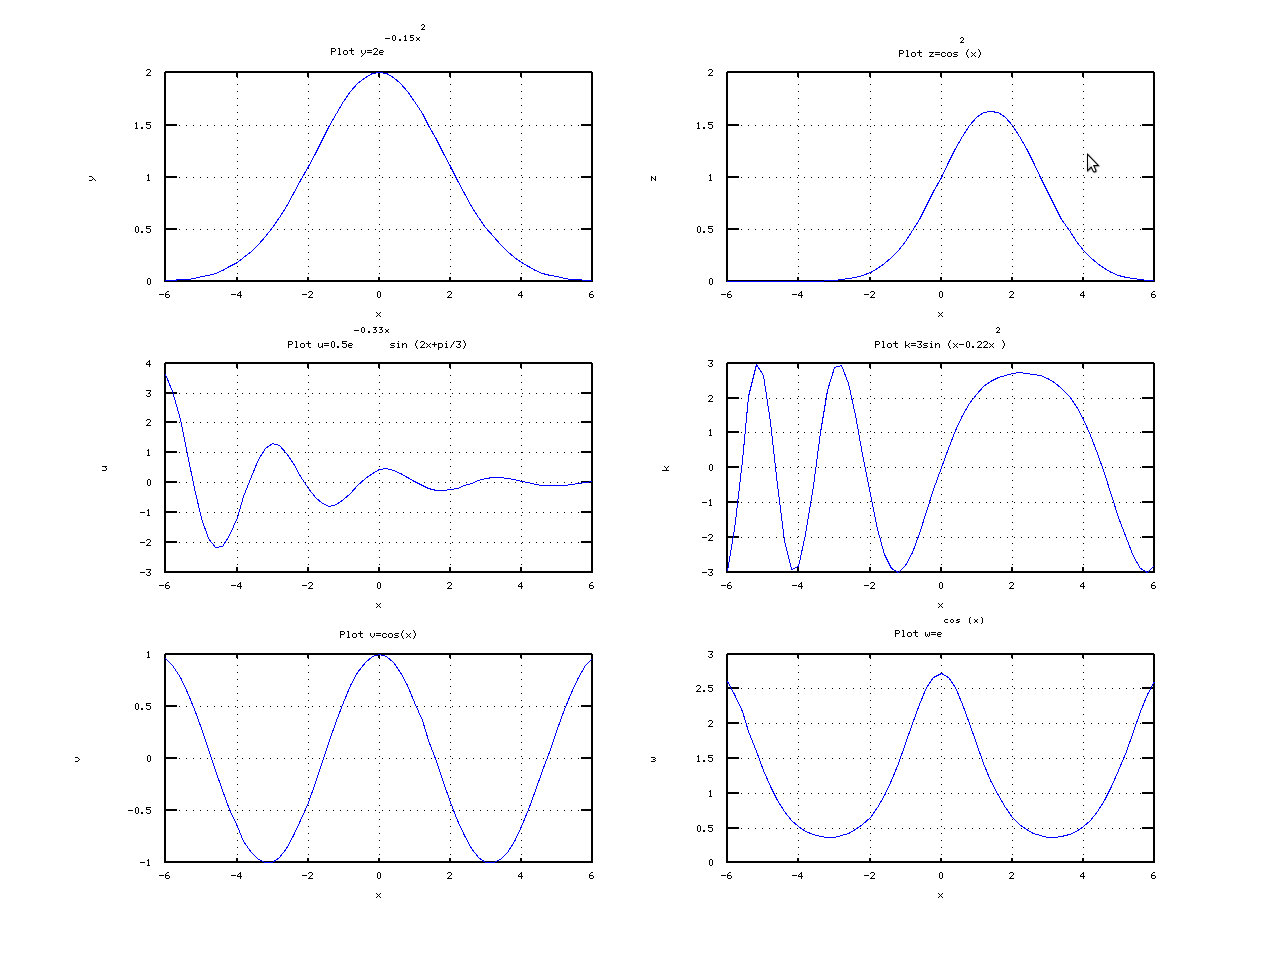
\includegraphics[width=8cm]{04_aer_octave_fig1.png}}
\caption{Графики графики нескольких функций в одном окне}
\label{pic:1}
\end{figure}

\begin{figure}[ht]
\centering{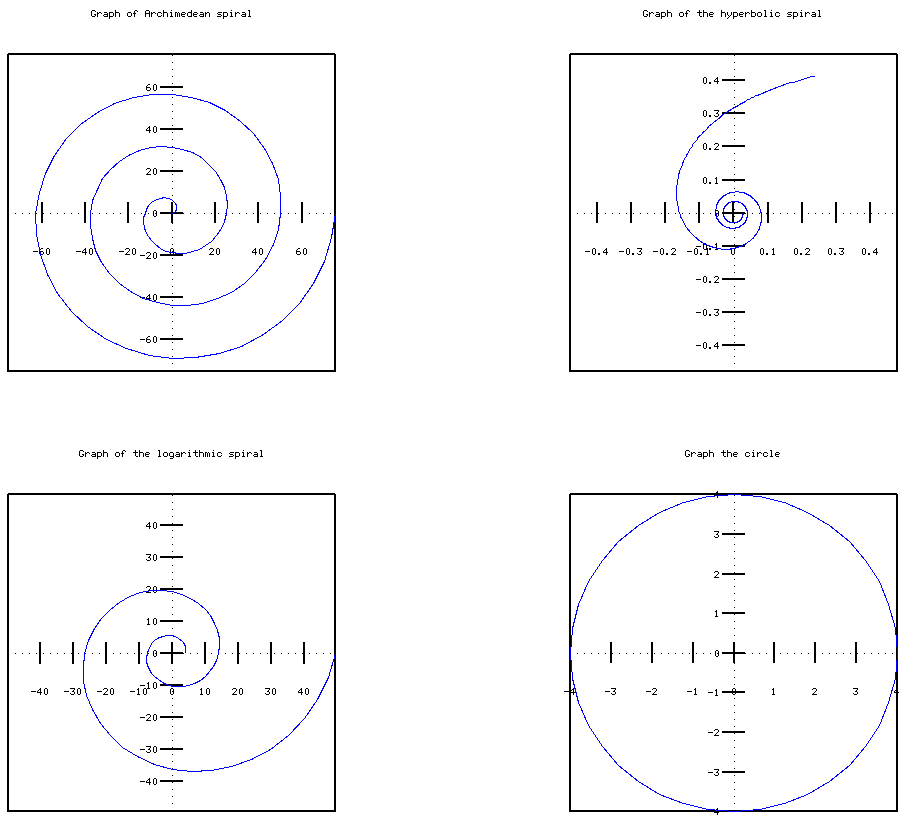
\includegraphics[width=8cm]{04_aer_octave_fig2.png}}
\caption{ Графики архимедовой, гиперболической и логарифмической спирали, окружности в полярных координатах}
\label{pic:2}
\end{figure}

\begin{figure}[ht]
\centering{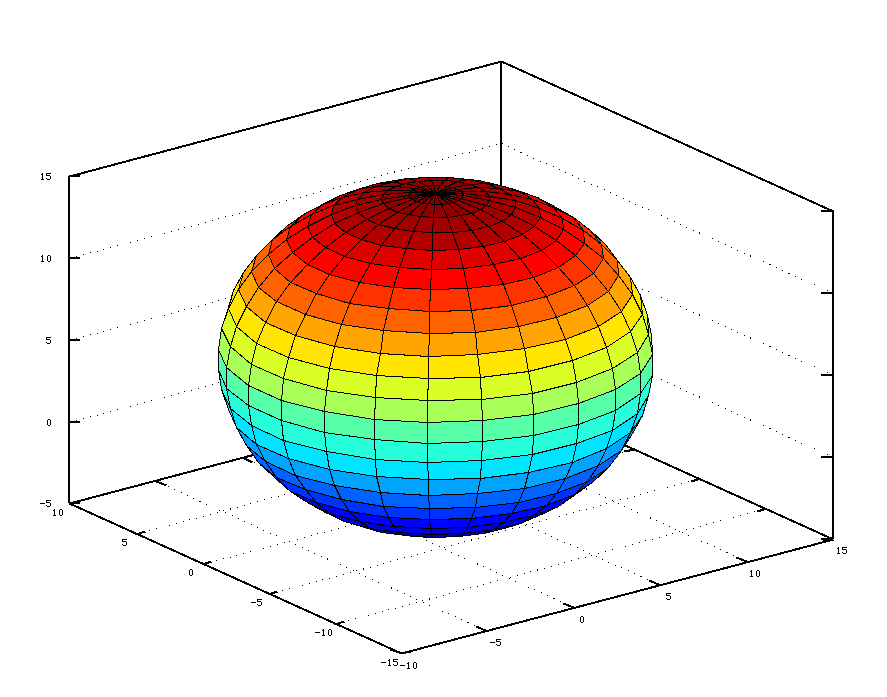
\includegraphics[width=8cm]{04_aer_octave_fig3.png}}
\caption{График сферы}
\label{pic:3}
\end{figure}

Octave содержит большое количество функций, предназначенных для решения задач линейной алгебры, наиболее используемые из них: \verb!det(M)! --- вычисляет определитель квадратной матрицы \verb!M!, \verb!norm(M[,p])! --- возвращает различные виды норм матрицы \verb!M! в зависимости от \verb!p!, \verb!inv(M)! --- возвращает матрицу обратную к \verb!M!, \verb!eig(M)! --- возвращает вектор собственных значений матрицы \verb!M!, \verb!rref(M)! --- осуществляет приведение матрицы \verb!M! к треугольной форме, используя метод исключения Гаусса, \verb!lu(M)!, \verb!qr (M)! --- выполняют LU и QR-разложение соответственно. 

Мощная графическая и математическая база  Octave позволяет решать задачи векторной алгебры и аналитической геометрии.

Octave содержит функции для численного и аналитического решения нелинейных уравнений и систем, а также для интегрирования и дифференцирования.

Оптимизационные задачи чаще всего решают с помощью проприетарного табличного процессора MS Excel. Однако, наиболее мощные и гибкие функции для решения подобных задач присутствуют именно в Octave. Так, для  решения линейных и нелинейных оптимизационных задач с ограничениями можно использовать функцию sqp, а для решения любых задач линейного программирования есть функция glpk. Сложные оптимизационные задачи в Octave решают с помощью пакета пакета расширений Minimization для GNU Octave (\url{http://octave.sourceforge.net/optim/overview.html}).

В инженерной практике часто приходится сталкиваться с решением обыкновенных дифференциальных уравнений и систем. В Octave существует достаточно много функций для решения обыкновенных уравнений и систем (в том числе и жёстких). Наиболее часто используемые среди них:
\begin{itemize}
\item \verb!ode23!, \verb!ode45! --- функции решений обыкновенных нежёстких дифференциальных уравнений (или систем) методом Рунге-Кутта 2-3-го и 4-5-го порядка точности соответсвенно,
\item \verb!ode5r!, \verb!ode2r! --- функции решений обыкновенных жёстких дифференциальных уравнений (или систем).
\end{itemize}

\begin{figure}[ht]
\centering{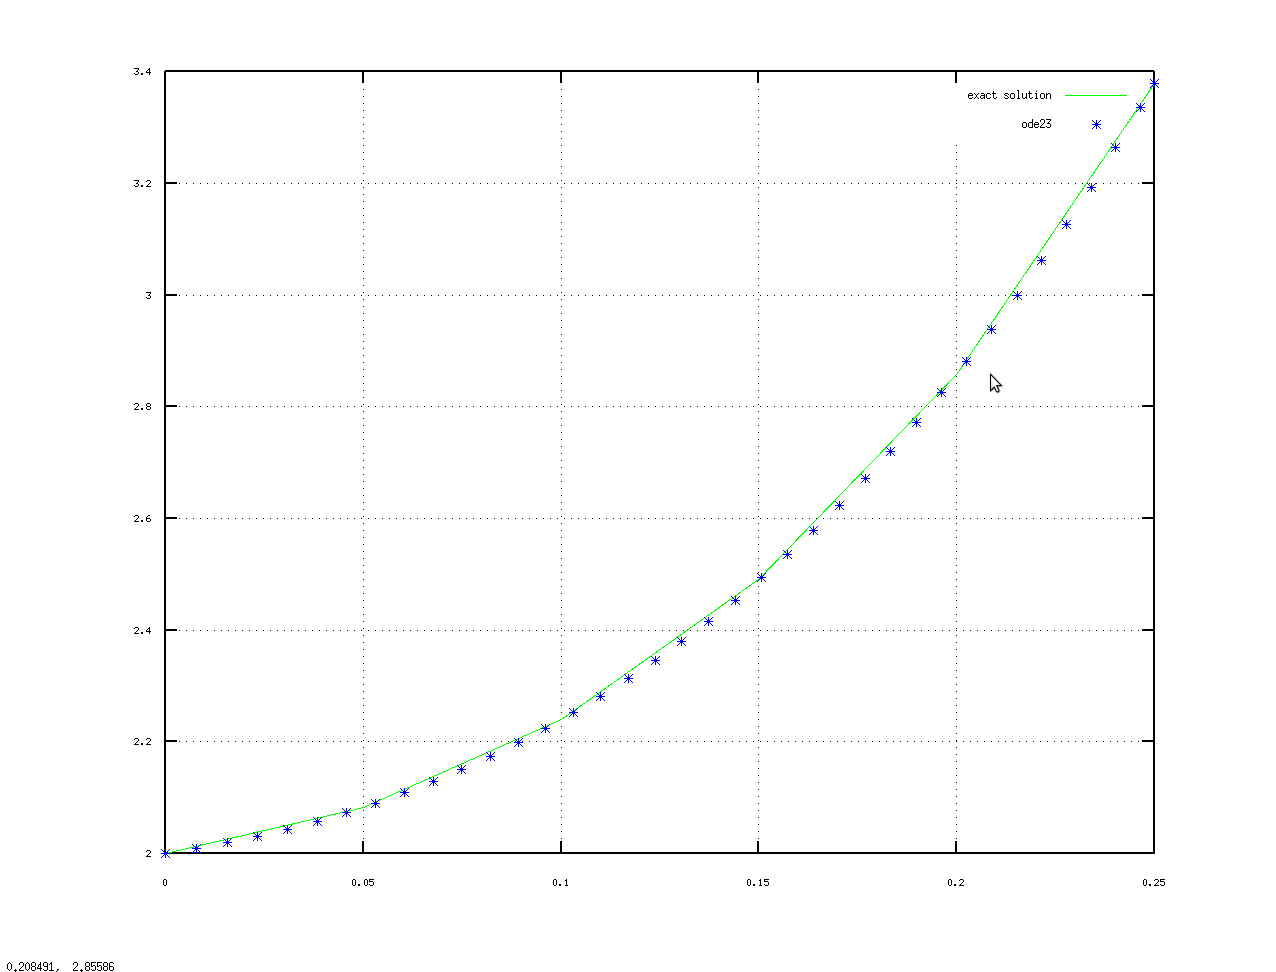
\includegraphics[width=8cm]{04_aer_octave_fig4.png}}
\caption{Графики точного решения (--) дифференциального уравнений и решения (*), найденного с помощью ode23}
\label{pic:4}
\end{figure}

Множество функций для решения дифференциальных уравнений находится в пакете расширений odepkg. Краткое описание функций этого пакета на английском языке с некоторыми примерами приведено на странице \url{http://octave.sourceforge.net/odepkg/overview.html}.

Также в Octave можно решать практически любые задачи обработки эксперимента. Для подбора параметров аналитической зависимости методом наименьших квадратов используются следующие функции: \verb!polyfit! --- подбор коэффициентов полинома k-й степени; \verb!sqp! --- функция поиска минимума.

Сплайн-интерполяция в Octave реализуется с помощью функции \verb!interp1!, которая позволяет  построить кубический и линейный сплайн.

C помощью Octave можно решать и много других задач. Авторами подготовлен учебник по использованию пакете GNU Octave, который будет опубликован в ближайшее время в Москве, в серии учебников ALT Linux, а также небольшим тиражом в Донецком национальном техническом университете. Рабочие материалы книги можно увидеть на сайте \url{http://gnu-octave.narod2.ru}.

Рассмотренные возможности Octave позволяют авторам рекомендовать пакет как инструмент для решения математических задач в курсах <<Высшая математика>>, <<Математический анализ>>, <<Линейная алгебра>>, <<Аналитическая геометрия>>, а также во многих специальных курсах, в которых приходится решать задачи вычислительной математики.
\end{document}





\documentclass[10pt, a5paper]{article}
\usepackage{pdfpages}
\usepackage{parallel}
\usepackage[T2A]{fontenc}
\usepackage{ucs}
\usepackage[utf8x]{inputenc}
\usepackage[polish,english,russian]{babel}
\usepackage{hyperref}
\usepackage{rotating}
\usepackage[inner=2cm,top=1.8cm,outer=2cm,bottom=2.3cm,nohead]{geometry}
\usepackage{listings}
\usepackage{graphicx}
\usepackage{wrapfig}
\usepackage{longtable}
\usepackage{indentfirst}
\usepackage{array}
\newcolumntype{P}[1]{>{\raggedright\arraybackslash}p{#1}}
\frenchspacing
\usepackage{fixltx2e} %text sub- and superscripts
\usepackage{icomma} % коскі ў матэматычным рэжыме
\PreloadUnicodePage{4}

\newcommand{\longpage}{\enlargethispage{\baselineskip}}
\newcommand{\shortpage}{\enlargethispage{-\baselineskip}}

\def\switchlang#1{\expandafter\csname switchlang#1\endcsname}
\def\switchlangbe{
\let\saverefname=\refname%
\def\refname{Літаратура}%
\def\figurename{Іл.}%
}
\def\switchlangen{
\let\saverefname=\refname%
\def\refname{References}%
\def\figurename{Fig.}%
}
\def\switchlangru{
\let\saverefname=\refname%
\let\savefigurename=\figurename%
\def\refname{Литература}%
\def\figurename{Рис.}%
}

\hyphenation{admi-ni-stra-tive}
\hyphenation{ex-pe-ri-ence}
\hyphenation{fle-xi-bi-li-ty}
\hyphenation{Py-thon}
\hyphenation{ma-the-ma-ti-cal}
\hyphenation{re-ported}
\hyphenation{imp-le-menta-tions}
\hyphenation{pro-vides}
\hyphenation{en-gi-neering}
\hyphenation{com-pa-ti-bi-li-ty}
\hyphenation{im-pos-sible}
\hyphenation{desk-top}
\hyphenation{elec-tro-nic}
\hyphenation{com-pa-ny}
\hyphenation{de-ve-lop-ment}
\hyphenation{de-ve-loping}
\hyphenation{de-ve-lop}
\hyphenation{da-ta-ba-se}
\hyphenation{plat-forms}
\hyphenation{or-ga-ni-za-tion}
\hyphenation{pro-gramming}
\hyphenation{in-stru-ments}
\hyphenation{Li-nux}
\hyphenation{sour-ce}
\hyphenation{en-vi-ron-ment}
\hyphenation{Te-le-pathy}
\hyphenation{Li-nux-ov-ka}
\hyphenation{Open-BSD}
\hyphenation{Free-BSD}
\hyphenation{men-ti-on-ed}
\hyphenation{app-li-ca-tion}

\def\progref!#1!{\texttt{#1}}
\renewcommand{\arraystretch}{2} %Іначай формулы ў матрыцы зліпаюцца з лініямі
\usepackage{array}

\def\interview #1 (#2), #3, #4, #5\par{

\section[#1, #3, #4]{#1 -- #3, #4}
\def\qname{LVEE}
\def\aname{#1}
\def\q ##1\par{{\noindent \bf \qname: ##1 }\par}
\def\a{{\noindent \bf \aname: } \def\qname{L}\def\aname{#2}}
}

\def\interview* #1 (#2), #3, #4, #5\par{

\section*{#1\\{\small\rm #3, #4. #5}}

\def\qname{LVEE}
\def\aname{#1}
\def\q ##1\par{{\noindent \bf \qname: ##1 }\par}
\def\a{{\noindent \bf \aname: } \def\qname{L}\def\aname{#2}}
}


\begin{document}
\renewcommand{\figurename}{Рыс.} % Не перакідаць у прэамбулу --- не працуе, чаму -- халера ведае.
\renewcommand{\abstractname}{Анатацыя}
\renewcommand{\refname}{Літаратура}

\title{Выкарыстанне свабоднага праграмнага забеспячэння ва ўстановах адукацыі Украіны: спроба аналізу}

\author{Грыгорый Злобiн\footnote{Львоўскі нацыянальны ўніверсітэт ім. Івана Франка, \url{zlobin@electronics.wups.lviv.ua}}}
\date{}

\maketitle

\begin{abstract}
The analysis of free / open source software usage in higher educational institutions of Ukraine is presented, based of the `FOSS Lviv-2011'  International Scientific Conference reports. 
\end{abstract}

Нягледзячы на станоўчы досвед выкарыстання свабодных праграм у адукацыі як у краінах блізкага, так і далёкага замежжа, ва Украіне да гэтага часу не прынятая канцэпцыя выкарыстання свабоднага праграмнага забеспячэння у адукацыі. Разам з тым намаганнямі энтузіястаў у навучальных установах Украіны свабоднае праграмнае забеспячэнне ўсё ж выкарыстоўваецца! Праз адасобленую пазіцыю Міністэрства адукацыі і навукі Украіны няма падрабязнай інфармацыі аб досведзе выкарыстання свабодных праграм у адукацыі. Дзякуючы таму, што ў Львоўскім нацыянальным універсітэце імя Івана Франка 01--06 лютага 2011 адбылася даволі прадстаўнічая міжнародная навукова"=практычная канферэнцыя <<FOSS Lviv-2011>>, з'явілася магчымасць правядзення аналізу выкарыстання СПЗ у вышэйшых навучальных установах Украіны. З 81 дакладаў 49 было прысвечана выкарыстанню СПЗ у навучальных установах. Даклады \cite{fosslviv}, якія былі пададзеныя на гэтую канферэнцыю, можна згрупаваць па наступных кірунках (назва дакладу падаецца на мове арыгіналу):

\section*{Дыстанцыйнае навучанне}
Гэтай тэматыцы прысвечаная найбольшая колькасць дакладаў "--- 10:
\begin{itemize}
\item <<Розроблення електронного деканату для системи управління дистанційним навчання MOODLE>> --- Артеменко В.Б., Львоўская камерцыйная акадэмія
\item <<Вибір платформи дистанційного навчання>> --- Коцаренко М.В., Бойко О.В.,  Львоўскі нацыянальны медыцынскі ўніверсітэт ім. Данііла Галіцкага
\item <<Використання контрольно-діагностичної програми iTest у ході моніторингу якості процесу навчання старшокласників>> --- Макаренко І.Є., Мерзлікін П.В., Крыварожскі дзяржаўны педагагічны ўніверсітэт
\item  <<Використання системи Moodle для організації контролю знань майбутніми вчителями-гуманітаріями>> --- Маркова Є.С., Бердзянскі дзяржаўны педагагічны ўніверсітэт
\item  <<Тестування в  Moodle як елемент менеджменту якості освіти: перший досвід>> --- Сергієнко В.П., Сліпухіна І.А., НПУ ім. М.П. Драгаманава
\item  <<Особливості програмного забезпечення в електронному навчанні>> --- Жарких Ю.С., Лисоченко С.В., Сусь Б.Б., Третяк О.В., Кіеўскі нацыянальны ўніверсітэт ім. Тараса Шаўчэнкі
\item  <<Інформаційно-аналітична система управління навчальним процесом ВНЗ на базі  Moodle>> --- Триус Ю.В., Чаркаскі дзяржаўны тэхналагічны ўніверсітэт
\item  <<Використання CMS JOMLA!  та LCMS MOODLE у ВНЗ>> --- Франчук В.М., НПУ ім. М.П. Драгаманава
\item <<Локалізація системи MOODLE " --- Франчук В.М., НПУ ім. М.П. Драгаманава
\item  <<Застосування вільного програмного забезпечення для дистанційного навчання у вищих навчальних закладах>> --- Захарченко В.М., Шапо В.М., Адэская нацыянальная марская акадэмія
\end{itemize}
\newpage

\section*{Выкарыстанне сістэм кампутарнай матэматыкі}
Наступныя 6 дакладаў можна аднесці да матэматычнай тэматыкі:
\begin{itemize}
\item <<Використання вільно-поширюваного ПЗ математичного призначення в університеті>> "--- Бугаєць Н.О., НПУ ім. М.П. Драгаманава
\item <<Вільнопоширювані системи комп'ютерної математики в осві\-ті і науці>> "--- Лазурчак І.І., Кобильник Т.П., Драгобыцкі дзяржаўны ўніверсітэт ім. І. Франка
\item <<Використання комп'ютерних математичних систем у про\-фе\-сій\-ній підготовці майбутнього вчителя математики>> "--- Лов'я\-но\-ва І.В., Крыварожскі дзяржаўны педагагічны ўніверсітэт
\item <<Моделювання задач електротехніки у XCOS>> "--- Філь І.М., Данецкі нацыянальны тэхнічны ўніверсітэт
\item <<Розробка і використання web-інтерфейсів для роботи з системами комп'ютерної математики>> "--- Чичкарьов Є.А., Прыазоўскі дзяржаўны тэхнічны ўніверсітэт
\item <<Про комп'ютерний супровід викладання геометрії>> "--- Яхненко І.В., Лутфулін М.В., Палтаўскі нацыянальны педагагічны ўніверсітэт ім. В.Г. Караленкі
\end{itemize}

\section*{Агульныя пытанні выкарыстання СПЗ у адукацыі}
7 дакладаў гэтай групы, якую можна прызнаць другой па колькасці, уключалі:
\begin{itemize}
\item <<Використання вільного програмного забезпечення в навчанні і наукових дослідженнях у Львівському національному уні\-вер\-ситеті імені Івана Франка>> "--- Апуневич С.Є., Злобін Г.Г., Рикалюк Р.Є., Шувар Р.Я., Львоўскі нацыянальны ўніверсітэт ім. І. Франка
\item <<Використання вільного програмного забезпечення в системі дистанційної освіти>> "--- Воронкін О.С., Луганскі дзяржаўны інстытут культуры і мастацтваў
\item <<Вільнопоширюване програмне забезпечення курсу “Нові інформаційні технології” для студентів спеціальності \linebreak “Біо\-ло\-гія”>> "--- Єфименко В.В., НПУ ім. М.П. Драгаманава
\item <<Використання вільного програмного забез\-печення у про\-фе\-сій\-ній підготовці майбутніх інженерів>> "--- Покришень Д.А., \linebreak Дрозд О.П., Сподаренко І.Й., Чарнігаўскі дзяржаўны тэхналагічны ўніверсітэт
\item  <<Про досвід використання ОС Linux у навчальному процесі Львівського національного медичного університету імені Данила Галицького>> "--- Риковський П.А., Львоўскі нацыянальны медыцынскі ўніверсітэт ім. Данііла Галіцкага
\item  <<LINUX  та VIRTUAL-BOX у навчанні абстрактних понять теорії операційних систем>> "--- Спірін О.М., Сверчевська О.С., Жытомірскі дзяржаўны ўніверсітэт ім. І. Франка
\item  <<З досвіду використання вільного програмного забезпечення при вивченні інформатики>> "--- Харченко В.М., Нежынскі дзяржаўны ўніверсітэт ім. М. Гогаля
\end{itemize}

\section*{Выкарыстанне адкрытых сродкаў праграмавання}
Гэтая група апынулася найменшай па колькасці і ўключае 4 даклады:
\begin{itemize}
\item <<Використання відкритих програмних засобів в процесі навчання статистичним дисциплінам>> "--- Коркуна Т.Й., Самбарскі тэхнікум эканомікі і інфарматыкі
\item <<Розрахунок фотоіонізаційних моделей небулярного газу в ОС LINUX UBUNTU 10.10 та WINDOWS 7>> "--- Мелех Б.Я., Тишко Н.Л., Коритко Р.І., Львоўскі нацыянальны ўніверсітэт ім. І. Франка
\item <<Реалізація розподілених обчислень на основі грід-платформи з відкритим кодом BOINC>> "--- Шийка Ю.Я., Шувар Р.Я., \linebreak Львоўскі нацыянальны ўніверсітэт ім. І. Франка
\item <<Реалізація високопродуктивної обчислювальної системи на базі ОС  LINUX>> "--- Шувар Р.Я., Бойко Я.В., Львоўскі нацыянальны ўніверсітэт ім. І. Франка
\end{itemize}

\section*{Распрацоўка праграмнага забеспячэння}
Будучы тэматычна-роднаснай папярэдняй, гэтая група больш шматлікая і складаецца з 7 дакладаў, яна зраўнавалася з катэгорыяй <<Агульныя пытанні выкарыстання СПЗ у адукацыі>>:
\begin{itemize}
\item <<Комплекс програм для лазерних спостережень штучних супутників Землі>> "--- Мартинюк-Лотоцький К.П., Білінський\linebreak А.\,І., Львоўскі нацыянальны ўніверсітэт ім. І. Франка
\item <<Розробка системи спектральної діагностики димової плазми>> "--- Сподарець Д.В., Драган Г.С., Адэскі нацыянальны ўні\-версітэт імя І.І. Мечнікава
\item <<Використання вільного програмного забез-печення для створення програми керування інформаційним автоматом>> "--- Зло\-бін Г., Скляр В., Чмихало О., Шевчик В., Львоўскі нацыянальны ўніверсітэт ім. І. Франка
\item <<Використання бібліотеки класів GEANT4 в ОС Linux при розробці програмного забезпечення для моделювання процесів взаємодії випромінювання з речовиною>> "--- Малихіна Т.В., Харкаўскі нацыянальны ўніверсітэт ім. В.Н. Каразіна
\item  <<Програма для обробкирезультатів ЛЛС-спостережень як \linebreak ВПЗ>> "--- Апуневич С.Є., Апуневич С.В., Білінський А.І., Благодир Я.Т., Львоўскі нацыянальны ўніверсітэт ім. І. Франка
\item  <<Програмне забезпечення керування телескопом  ЛЛС-станції Львів-1831>> "--- Білінський А.І., Мартинюк-Лотоцький К.\,П., \linebreak Львоўскі нацыянальны ўніверсітэт ім. І. Франка
\item <<Використання Open Wrt як основи вбудованого програмного забезпечення маршрутизаторів>> "--- Нек Т., Львоўскі нацыянальны ўніверсітэт ім. І. Франка
\end{itemize}

\section*{Асобныя даклады}
І нарэшце, 5 дакладаў немагчыма аднесці ні да адной з пералічаных вышэй катэгорый:
\begin{itemize}
\item  <<Інформаційна технологія управління навчальним навантаженням у вищих навчальних закладах>> "--- Гриценко В.Г., Чаркаскі нацыянальны ўніверсітэт ім. Б. Хмяльніцкага
\item  <<Про досвід використання офісного  пакету OpenOffice.org.ukr в курсі інформатики для економічних і юридичних спеціальностей ВЗО>> "--- Злобін Г.Г., Львоўскі нацыянальны ўніверсітэт ім. І. Франка 
\item  <<Досвід використання  редактора Gimp при вивченні курсу “Комп'ютерна графіка і дизайн”>> "--- Матвієнко Ю.С., Палтаўскі нацыянальны педагагічны ўніверсітэт ім. В.Г. Караленкі
\item <<Використання програми GANTTPROJECT для побудови календарних графіків при розробці ПВР>> "--- Грицук Ю.В., Меліхов О.І., Данбаская акадэмія будаўніцтва і архітэктуры
\item <<Вільне ПЗ для підготовки наукових текстів і презентацій>> "--- Лутфуллін М.В., Моторний М.І., Палтаўскі нацыянальны педагагічны ўніверсітэт ім. В.Г. Караленкі
\end{itemize}

	Такім чынам, можна канстатаваць як шырокі спектр выкарыстання СПЗ ва ўкраінскіх навучальных установах ад дыстанцыйнага навучання да распрацоўкі адкрытага праграмнага забеспячэння, так і шырокую геаграфію выкарыстання СПЗ ад Луганска на ўсходзе да Львова на захадзе і ад Чарнігава на поўначы да Адэсы на поўдні (глядзі рыс.).

\begin{figure}[ht]
\centering{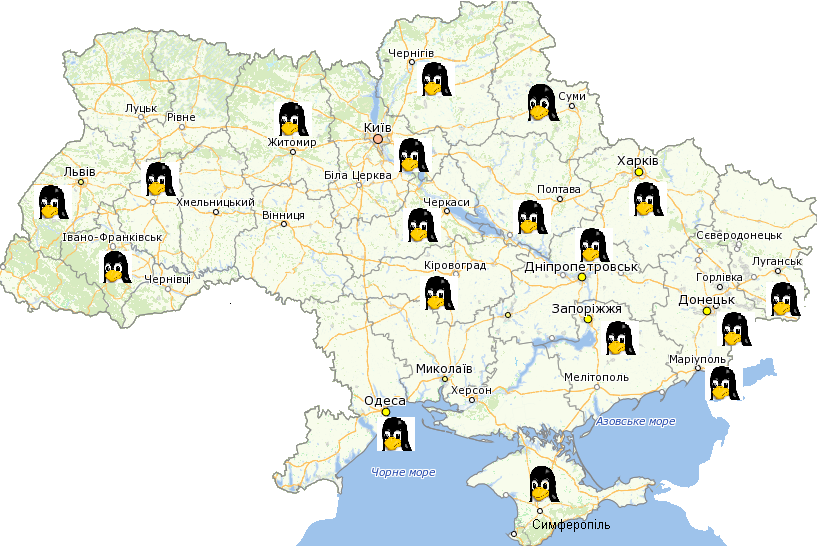
\includegraphics[width=8cm]{05_ukraine_linux.png}}
\label{pic:fl1}
%\caption{~}
\end{figure}

\begin{thebibliography}{9}
\bibitem{fosslviv}Тези міжнародної науково-практичної конференції FOSS LVIV-2011. Збірник наукових праць /за ред. Злобіна Г.Г., Апуневича С.Є., Машкова В.В., Апуневич С.В. Вид-во ЛНУ імені Івана Франка. 2011. --- 196 с.
\end{thebibliography}

\end{document}





\documentclass[a5paper,10pt]{article}
\usepackage{pdfpages}
\usepackage{parallel}
\usepackage[T2A]{fontenc}
\usepackage{ucs}
\usepackage[utf8x]{inputenc}
\usepackage[polish,english,russian]{babel}
\usepackage{hyperref}
\usepackage{rotating}
\usepackage[inner=2cm,top=1.8cm,outer=2cm,bottom=2.3cm,nohead]{geometry}
\usepackage{listings}
\usepackage{graphicx}
\usepackage{wrapfig}
\usepackage{longtable}
\usepackage{indentfirst}
\usepackage{array}
\newcolumntype{P}[1]{>{\raggedright\arraybackslash}p{#1}}
\frenchspacing
\usepackage{fixltx2e} %text sub- and superscripts
\usepackage{icomma} % коскі ў матэматычным рэжыме
\PreloadUnicodePage{4}

\newcommand{\longpage}{\enlargethispage{\baselineskip}}
\newcommand{\shortpage}{\enlargethispage{-\baselineskip}}

\def\switchlang#1{\expandafter\csname switchlang#1\endcsname}
\def\switchlangbe{
\let\saverefname=\refname%
\def\refname{Літаратура}%
\def\figurename{Іл.}%
}
\def\switchlangen{
\let\saverefname=\refname%
\def\refname{References}%
\def\figurename{Fig.}%
}
\def\switchlangru{
\let\saverefname=\refname%
\let\savefigurename=\figurename%
\def\refname{Литература}%
\def\figurename{Рис.}%
}

\hyphenation{admi-ni-stra-tive}
\hyphenation{ex-pe-ri-ence}
\hyphenation{fle-xi-bi-li-ty}
\hyphenation{Py-thon}
\hyphenation{ma-the-ma-ti-cal}
\hyphenation{re-ported}
\hyphenation{imp-le-menta-tions}
\hyphenation{pro-vides}
\hyphenation{en-gi-neering}
\hyphenation{com-pa-ti-bi-li-ty}
\hyphenation{im-pos-sible}
\hyphenation{desk-top}
\hyphenation{elec-tro-nic}
\hyphenation{com-pa-ny}
\hyphenation{de-ve-lop-ment}
\hyphenation{de-ve-loping}
\hyphenation{de-ve-lop}
\hyphenation{da-ta-ba-se}
\hyphenation{plat-forms}
\hyphenation{or-ga-ni-za-tion}
\hyphenation{pro-gramming}
\hyphenation{in-stru-ments}
\hyphenation{Li-nux}
\hyphenation{sour-ce}
\hyphenation{en-vi-ron-ment}
\hyphenation{Te-le-pathy}
\hyphenation{Li-nux-ov-ka}
\hyphenation{Open-BSD}
\hyphenation{Free-BSD}
\hyphenation{men-ti-on-ed}
\hyphenation{app-li-ca-tion}

\def\progref!#1!{\texttt{#1}}
\renewcommand{\arraystretch}{2} %Іначай формулы ў матрыцы зліпаюцца з лініямі
\usepackage{array}

\def\interview #1 (#2), #3, #4, #5\par{

\section[#1, #3, #4]{#1 -- #3, #4}
\def\qname{LVEE}
\def\aname{#1}
\def\q ##1\par{{\noindent \bf \qname: ##1 }\par}
\def\a{{\noindent \bf \aname: } \def\qname{L}\def\aname{#2}}
}

\def\interview* #1 (#2), #3, #4, #5\par{

\section*{#1\\{\small\rm #3, #4. #5}}

\def\qname{LVEE}
\def\aname{#1}
\def\q ##1\par{{\noindent \bf \qname: ##1 }\par}
\def\a{{\noindent \bf \aname: } \def\qname{L}\def\aname{#2}}
}


\begin{document}


\title{Облачные вычисления и сервисы: классификация, основные функции, преимущества и недостатки}

\author{Виталий Сороко\footnote{Минск, \url{http://arneta.ru}}}

\maketitle
\begin{abstract}
In the past, big part of computer-related activity was impos\-sible without the installation of software to a local computer, but now, with help of cloud services, users can perform such typical tasks as word processing within their web-browser. It becomes possible due to so called cloud-based resources. Here an attempt of  cloud technologies and systems general overview is presented with the technical description of the architecture, characteristics and features comparison. 
\end{abstract}

Среди наиболее полных определений облачных систем на сегодняшний день можно выделить следующие два:
\begin{itemize}
\item Облачные сервисы "--- это технология обработки данных, в которой программное обеспечение предоставляется пользователю как интернет-сервис, при котором от пользователя скрыта инфраструктура <<облака>> (облачной системы) и, поэтому, ему не требуются специальные знания и навыки для  управления и использования данной <<облачной>> технологии.
\item Облачные вычисления "--- это вычисления, которые представляют собой динамически масштабируемый способ доступа к внешним вычислительным ресурсам в виде сервиса, предоставляемого посредством Интернета.
\end{itemize}

Данные определения тесно связаны между собой: для реализации всех облачных сервисов необходимы вычисления, а облачные вычисления по сути сами являются облачным сервисом. Рассмотрим классификацию облачных сервисов и их реализаций из мира свободного ПО.

В настоящее время все облачные сервисы подразделяют на:
\begin{itemize}
\item \emph{«Программное обеспечение как услуга»} (Software as a Service, сокращённо SaaS) "--- бизнес-модель продажи программного \linebreak обеспечения, при которой владелец (поставщик) ПО предоставляет доступ к к нему пользователям (заказчикам) через Интернет. Примерами такого ПО являются Feng Office Community Edition, Simple Groupware, Zarafa и др.
\item \emph{«Оборудование (вычислительные мощности) как услуга»} \linebreak (Hardware as a Service, сокращённо HaaS) "--- предоставление  вычислительных ресурсов оборудования (его процессорного времени, места для место под хранения данных и т.д.) в виде сервисов с использованием технологий виртуализации. Сервисы обычно предлагаются как эквивалент реальным вычислительным системам, таким как серверы, суперкомпьютеры и др. Над программной реализацией этой идеи полностью или частично работают проекты OpenVZ, FreeVPS, Linux-VServer, Apache Hama, GlusterFS Open Source Project, а также Moose File System (MooseFS) и др., а предоставляет такой сервис на базе OpenSource решений компания Linode и некоторые другие.
\item \emph{<<Коммуникация как Сервис>>} (Communications as a Service, сокр. CaaS) "--- построенное в облаке коммуникационное решение для предприятия, которое обеспечивает передачу речевого сигнала по сети Интернет или по любым другим IP-сетям (VoIP), обмен мгновенными сообщениями (IM), видеоконференции. Модель CaaS позволяет деловым клиентам выборочно разворачивать средства коммуникаций и услуг на оснований оплаты услуг в срок для используемых сервисов. С этим направлением тесно связаны такие FOSS-проекты как Ekiga, iLBC, Speex.
\item \emph{«Мониторинг как Сервис»} (Monitoring-as-a-Service, сокращённо MaaS) является обслуживаемым в облаке программным обеспечением для мониторинга и обеспечения безопасности. Такими OpenSource-решениями на сегодняшний день являются Ganglia, Zabbix, Hyperic HQ. Сюда же  с некоторыми оговорками модно отнести и Nagios. 
\item \emph{«Инфраструктура как услуга»} (Infrastructure as a Service, сокращённо IaaS) "--- это предоставление компьютерной инфраструктуры (как правило в форме виртуализации) как услуги на основе концепции облачных вычислений. По сути IaaS является комбинацией SaaS,  HaaS, так как она включает в себя и то и другое, причем обычно во множественном числе, а также CaaS и иногда MaaS с целью объедения и мониторинга всей системы, и, поэтому, используется в основном предприятиями. Свободными реализациями данной концепции являются Eucalyptus, OpenNebula, OpenStack, Nimbus и др.
\item \emph{«Платформа как услуга»} (Platform as a Service, сокр. PaaS) "--- предоставление программной платформы и инструментов с определенными характеристиками, необходимых для разработки, тестирования, развертывания, поддержки различных приложений. Сюда же входят и готовые к использованию облачные сервисы, которые вместе образуют программную платформу. Яркими примерами из мира OpenSource в настоящее время являются Xen Cloud Platform, Cloud Foundry, Apache Hadoop, Apache Hive и др.
\item \emph{«Компьютер (виртуальный рабочий стол) как услуга»} (Desk\-top as a Service, сокращённо DaaS) "--- предоставление виртуального компьютера, который каждый пользователь может индивидуально настраивать под свои задачи. Таким образом, пользователь приходя на работу просто вводит свои данные (обычно логин и пароль) и может работать, используя при этом благодаря технологиям виртуализации вычислительные мощности стороннего сервера, а не своего ПК. 
\item \emph{<<Рабочее окружение как услуга>>} (Workspace as a Service, сокращённо WaaS) "--- предоставление комплекта  SaaS, предназначенного для создания рабочего окружения. В отличие от DaaS в этом случае пользователь получает доступ только к ПО, в то время как все вычисления происходят непосредственно на его машине. По сути данная категория является гибридом SaaS и PaaS, так как в отличие от последней является платформой, направленной не на разработку и тестирование ПО, а на офисную работу, но при этом как первая в реализации не использует технологий виртуализации. На данный момент реализации данной технологии предоставляются в основном различными крупными компаниями, например Google и Microsoft, и представляют в основном решения с закрытым исходным кодом, иногда с использованием свободных и открытых компонентов или их исходников.
\item \emph{«Все как услуга»} (Everything as a service, сокращённо EaaS) "--- концептуальная модель, включающая в себя элементы всех перечисленных решений. На данный момент полной её реализации не существует "--- она по сути является идеалом для крупных облачных компаний, таких как Google и Microsoft.
\end{itemize}

Свободное и открытое программное обеспечение в настоящее время играет ключевую роль в создании и развертывании облачных сервисов и систем. С одной стороны существуют ряд созданных сообществом платформ, ориентированных на облачные вычисления (Xen, Eucaliptus, Cloud Foundry, Feng Office и др.). С другой стороны, само свободное ПО (операционные системы семейства Linux и BSD, Web-браузеры и т.\,д.) как нельзя лучше подходит для размещения и использования облачных сервисов.  Естественно, что существует и целый ряд проприетарных аналогов.

Рыночная доля облачных сервисов и платформ постоянно растет благодаря ряду преимуществ для обычных пользователей и организаций, среди которых в первую очередь можно отметить:
\begin{itemize}
\item	количество процессоров, объем оперативной памяти и дискового пространства в облачных системах теоретически ничем не ограничен;
\item	пользователям не нужно самостоятельно устанавливать и настраивать ПО, т.\,к. для доступа к облачным сервисам достаточно обычного web-браузера;
\item	пользователям не нужно покупать дорогое оборудование;
\item	экономия времени и энергии на выполнение некоторых задач, а также, в особых случаях, и площадей, занимаемых оборудованием;
\item	возможность производить оплату только за потребленные вычислительные мощности и произведенные операции;
\item	в организациях отсутствуют затраты на развёртывание инфраструктуры;
\item	организации получают сокращение затрат на техническую поддержку и обновление развернутых систем, а также высокую скорость внедрения, обусловленную отсутствием временных затрат на развертывание системы;
\item	отсутствует необходимость обучения "--- большинство пользователей уже умеют пользоваться web-браузерами и интернет-сервисами как классом услуг;
\item	обычно облачные системы обслуживаются высококвалифицированными профессионалами, что дает более высокий уровень качества обслуживания ПО.
\end{itemize}

Тем не менее облачные системы не лишены недостатков, которые в большей степени касаются обычных пользователей, и в меньшей --- провайдеров:
\begin{itemize}
\item из-за вопросов безопасности не все данные можно доверить стороннему провайдеру, тем более, не только для хранения, но и для обработки;
\item далеко не каждое облачное приложение позволяет сохранить полученные результаты в удобном для пользователя виде на нужный носитель данных;
\item риск массовой потери данных многими пользователями из-за технического сбоя у поставщика облачных услуг;
\item потеря свободы "--- большая часть облачных сервисов не имеет четких стандартов, и поэтому при переходе от одного поставщика облачных услуг к другому могут возникнуть серьезные проблемы. Они же могут возникнуть и при обновлении провайдером собственных облачных сервисов "--- если, например, он пожелает внедрить новый интерфейс, то подписчикам придётся им пользоваться.  Немаловажным моментом также является необходимость доступа в интернет, что в некоторых случаях ведет к потере свободы перемещений. А главное, благодаря тому, что все данные находятся в руках провайдера, нельзя исключать того, что недобросовестные компании могут воспользоваться этим.
\end{itemize}

Можно предположить, что как сейчас большая часть пользователей использует Windows и Microsoft Office, так в ближайшем будущем эти пользователи оценят преимущества облачных платформ и перейдут на них. При этом, даже передумав после получения очередной порции счетов за оплату сервисов, пользователям будет трудно вернуться к прежней схеме работы "--- все их данные будут в руках компании"=владельца облачной системы, а для самостоятельной установки другой операционной системы и иного программного обеспечения многим не хватит квалификации, да и приобретённое пользователями оборудование скорее всего будет иметь крайне малую мощность. В этом случае эффективным выходом оказывается  свободное ПО, которое как правило способно работать на маломощном оборудовании при сохранении совместимости со старыми системами. В этом случае возврат пользователей из облака также едва ли станет массовым, поскольку крупные облачные компании постараются сделать этот переход невыгодным, если не невозможным, однако сам факт такой возможности будет являться дополнительным регулирующим фактором, ограничивающим прибыли провайдеров облачных услуг.

\end{document}

\documentclass[10pt, a5paper]{article}
\usepackage{pdfpages}
\usepackage{parallel}
\usepackage[T2A]{fontenc}
\usepackage{ucs}
\usepackage[utf8x]{inputenc}
\usepackage[polish,english,russian]{babel}
\usepackage{hyperref}
\usepackage{rotating}
\usepackage[inner=2cm,top=1.8cm,outer=2cm,bottom=2.3cm,nohead]{geometry}
\usepackage{listings}
\usepackage{graphicx}
\usepackage{wrapfig}
\usepackage{longtable}
\usepackage{indentfirst}
\usepackage{array}
\newcolumntype{P}[1]{>{\raggedright\arraybackslash}p{#1}}
\frenchspacing
\usepackage{fixltx2e} %text sub- and superscripts
\usepackage{icomma} % коскі ў матэматычным рэжыме
\PreloadUnicodePage{4}

\newcommand{\longpage}{\enlargethispage{\baselineskip}}
\newcommand{\shortpage}{\enlargethispage{-\baselineskip}}

\def\switchlang#1{\expandafter\csname switchlang#1\endcsname}
\def\switchlangbe{
\let\saverefname=\refname%
\def\refname{Літаратура}%
\def\figurename{Іл.}%
}
\def\switchlangen{
\let\saverefname=\refname%
\def\refname{References}%
\def\figurename{Fig.}%
}
\def\switchlangru{
\let\saverefname=\refname%
\let\savefigurename=\figurename%
\def\refname{Литература}%
\def\figurename{Рис.}%
}

\hyphenation{admi-ni-stra-tive}
\hyphenation{ex-pe-ri-ence}
\hyphenation{fle-xi-bi-li-ty}
\hyphenation{Py-thon}
\hyphenation{ma-the-ma-ti-cal}
\hyphenation{re-ported}
\hyphenation{imp-le-menta-tions}
\hyphenation{pro-vides}
\hyphenation{en-gi-neering}
\hyphenation{com-pa-ti-bi-li-ty}
\hyphenation{im-pos-sible}
\hyphenation{desk-top}
\hyphenation{elec-tro-nic}
\hyphenation{com-pa-ny}
\hyphenation{de-ve-lop-ment}
\hyphenation{de-ve-loping}
\hyphenation{de-ve-lop}
\hyphenation{da-ta-ba-se}
\hyphenation{plat-forms}
\hyphenation{or-ga-ni-za-tion}
\hyphenation{pro-gramming}
\hyphenation{in-stru-ments}
\hyphenation{Li-nux}
\hyphenation{sour-ce}
\hyphenation{en-vi-ron-ment}
\hyphenation{Te-le-pathy}
\hyphenation{Li-nux-ov-ka}
\hyphenation{Open-BSD}
\hyphenation{Free-BSD}
\hyphenation{men-ti-on-ed}
\hyphenation{app-li-ca-tion}

\def\progref!#1!{\texttt{#1}}
\renewcommand{\arraystretch}{2} %Іначай формулы ў матрыцы зліпаюцца з лініямі
\usepackage{array}

\def\interview #1 (#2), #3, #4, #5\par{

\section[#1, #3, #4]{#1 -- #3, #4}
\def\qname{LVEE}
\def\aname{#1}
\def\q ##1\par{{\noindent \bf \qname: ##1 }\par}
\def\a{{\noindent \bf \aname: } \def\qname{L}\def\aname{#2}}
}

\def\interview* #1 (#2), #3, #4, #5\par{

\section*{#1\\{\small\rm #3, #4. #5}}

\def\qname{LVEE}
\def\aname{#1}
\def\q ##1\par{{\noindent \bf \qname: ##1 }\par}
\def\a{{\noindent \bf \aname: } \def\qname{L}\def\aname{#2}}
}

\begin{document}
\title{Cистема распределенного выполнения задач paexec }
\author{Алексей Чеусов\\
\small Минск, Беларусь}
\def\progref!#1!{\texttt{#1}}

\maketitle

\begin{abstract}paexec distributes tasks across several CPUs or machines in a
network and collects results from those CPUs/machines. paexec runs
several instances of ``calculator'' on remote/local machines and sends
them tasks one by one recieving results from them. ``tasks'' given on
input may be either a list of independent tasks or a dependency
graph. ``transport'' is any rsh/ssh-like program. Cool features:
resistance to network failures, minimization of total calculation
time.
\end{abstract}

В последнее время все большее распространение получают компьютерные
системы оснащенные большим количеством процессоров или ядер.  В
настоящее время многоядерными процессорами комплектуются не только
мощные сервера и рабочие станции, но также ноутбуки, нетбуки и
даже мобильные телефоны и планшеты. В связи с этим часто возникает
задача распараллеливания выполнения задач с использованием всех
имеющихся вычислительных ресурсов. Та же проблема возникает при
использовании кластера компьютеров, объединенных в вычислительную
сеть. Задача не нова, и для ее решения имеется масса инструментов,
таких, например, как MPI, стандартный API (реализован в библиотеках
openmpi, mpich и др.), широко применяемый математиками для расчетов на
супер-ЭВМ и кластерах.  Тем не менее, существующие инструменты не
лишены недостатков.  В силу лицензионных ограничений далеко не всегда
имеющиеся инструменты можно легально использовать в коммерческих
целях, часто они имеют весьма специфическую область применения и
неудобны для решения простых пользовательских задач, существующие
инструменты порой слишком требовательны к количеству оперативной
памяти и дискового пространства, а то и просто ограничены конкретной
программно-аппаратной архитектурой.

Задача, ставшая в свое время перед автором --- обработка больших
массивов информации, а позднее обработка дерева задач, с
использованием нескольких компьютеров различной аппаратной
архитектуры. При этом <<задача>> в моем случае решалась автономной
программой, написанной с применением различных языков
программирования. Не найдя готового решения, подходящего для моего
случая, я разработал программный пакет paexec с открытым исходным
кодом (лицензия MIT), и разместил его в сети Интернет для публичного
доступа.

Домашняя страница проекта: \url{http://paexec.sf.net/}.

\section*{Как это работает}
В программный пакет paexec входят на данный момент
две программы, главная из которых -- paexec(1), собственно инструмент для
распараллеливания, получающий в качестве аргументов
\begin{enumerate}
\item \emph{задачи} для выполнения. Каждая отдельная задача --- это
   произвольная текстовая строка, не содержащая пробелов. Это может
   быть, например, имя файла, формула для вычисления и
   т.п. Совокупность же задач может представлять собой множество
   независимых задач, то есть задач, которые могут выполняться
   параллельно, либо орграф, узлами в котором являются задачи, а ребро
   $(A, B)$ означает: <<для выполнения задачи $B$ необходимо сначала
   выполнить задачу $A$; если задача $A$ по каким-либо причинам не смогла
   быть выполнена, пометить задачу $B$ и все другие задачи, зависящие от
   A как невыполненные>>. В целях задания порядка выполнения задач,
   каждой их них можно поставить в соответствии некоторый вес,
   определяющий, в какой момент лучше начать ее обработку. Реализовано
   несколько механизмов учета данных весов. В качестве веса можно,
   например, выбрать приблизительное время выполнения задачи или ее
   важность.
\item \emph{список узлов}, на которых, будут производится вычисления, узлами
   могут быть, например, имена компьютеров в сети или номера процессоров,
   адреса chroot пространств на UNIX"=системе и т.д.
\item \emph{вычислитель}. Это программа, принимающая на вход задачу для
   вычисления и печатающая на стандартный поток вывода результаты в
   определенном формате.
\item \emph{транспорт}, задающий способ связи с узлами, им могут быть такие
   программы как rsh, ssh или любые другие с совместимым способом
   использования. В случае, если транспорт не указан, \emph{вычислители}
   будут запущены локально указанное число раз.
\end{enumerate}

На стандартный поток вывода \progref!paexec(1)! выдает результат обработки задач
вычислителями (последовательность текстовых \linebreak строк) в порядке их
поступления от вычислительных узлов (sliced output). Вторая программа,
входящая в комплект --- \progref!paexec\_re\-order(1)!, она предназначена для
пересортировки выходного потока \progref!paexec(1)!.

Важно отметить, что \progref!paexec(1)! устойчив к сбоям в сети, а это значит,
может использоваться даже в сетях с неустойчивой связью, таких,
например, как Интернет. Устойчивость заключается в том, что в случае
потери связи с узлом, переданная ему на выполнение задача
перераспределится на другой свободный узел в момент его появления.
Периодически происходит попытка восстановления связи с узлами, связь с
которыми была потеряна.

\section*{Success stories}
На базе программного пакета paexec разработана
распределенная система сборки программных пакетов pkgsrc
(pkgtools/dist\-bb), успешно применяемая в течение многих лет на таких
операционных системах как NetBSD, Linux, Solaris, FreeBSD и др. Также,
paexec успешно применяется в компании Invention Machine для
распределенной обработки данных.
\end{document}

\documentclass[10pt, a5paper]{article}
\usepackage{pdfpages}
\usepackage{parallel}
\usepackage[T2A]{fontenc}
\usepackage{ucs}
\usepackage[utf8x]{inputenc}
\usepackage[polish,english,russian]{babel}
\usepackage{hyperref}
\usepackage{rotating}
\usepackage[inner=2cm,top=1.8cm,outer=2cm,bottom=2.3cm,nohead]{geometry}
\usepackage{listings}
\usepackage{graphicx}
\usepackage{wrapfig}
\usepackage{longtable}
\usepackage{indentfirst}
\usepackage{array}
\newcolumntype{P}[1]{>{\raggedright\arraybackslash}p{#1}}
\frenchspacing
\usepackage{fixltx2e} %text sub- and superscripts
\usepackage{icomma} % коскі ў матэматычным рэжыме
\PreloadUnicodePage{4}

\newcommand{\longpage}{\enlargethispage{\baselineskip}}
\newcommand{\shortpage}{\enlargethispage{-\baselineskip}}

\def\switchlang#1{\expandafter\csname switchlang#1\endcsname}
\def\switchlangbe{
\let\saverefname=\refname%
\def\refname{Літаратура}%
\def\figurename{Іл.}%
}
\def\switchlangen{
\let\saverefname=\refname%
\def\refname{References}%
\def\figurename{Fig.}%
}
\def\switchlangru{
\let\saverefname=\refname%
\let\savefigurename=\figurename%
\def\refname{Литература}%
\def\figurename{Рис.}%
}

\hyphenation{admi-ni-stra-tive}
\hyphenation{ex-pe-ri-ence}
\hyphenation{fle-xi-bi-li-ty}
\hyphenation{Py-thon}
\hyphenation{ma-the-ma-ti-cal}
\hyphenation{re-ported}
\hyphenation{imp-le-menta-tions}
\hyphenation{pro-vides}
\hyphenation{en-gi-neering}
\hyphenation{com-pa-ti-bi-li-ty}
\hyphenation{im-pos-sible}
\hyphenation{desk-top}
\hyphenation{elec-tro-nic}
\hyphenation{com-pa-ny}
\hyphenation{de-ve-lop-ment}
\hyphenation{de-ve-loping}
\hyphenation{de-ve-lop}
\hyphenation{da-ta-ba-se}
\hyphenation{plat-forms}
\hyphenation{or-ga-ni-za-tion}
\hyphenation{pro-gramming}
\hyphenation{in-stru-ments}
\hyphenation{Li-nux}
\hyphenation{sour-ce}
\hyphenation{en-vi-ron-ment}
\hyphenation{Te-le-pathy}
\hyphenation{Li-nux-ov-ka}
\hyphenation{Open-BSD}
\hyphenation{Free-BSD}
\hyphenation{men-ti-on-ed}
\hyphenation{app-li-ca-tion}

\def\progref!#1!{\texttt{#1}}
\renewcommand{\arraystretch}{2} %Іначай формулы ў матрыцы зліпаюцца з лініямі
\usepackage{array}

\def\interview #1 (#2), #3, #4, #5\par{

\section[#1, #3, #4]{#1 -- #3, #4}
\def\qname{LVEE}
\def\aname{#1}
\def\q ##1\par{{\noindent \bf \qname: ##1 }\par}
\def\a{{\noindent \bf \aname: } \def\qname{L}\def\aname{#2}}
}

\def\interview* #1 (#2), #3, #4, #5\par{

\section*{#1\\{\small\rm #3, #4. #5}}

\def\qname{LVEE}
\def\aname{#1}
\def\q ##1\par{{\noindent \bf \qname: ##1 }\par}
\def\a{{\noindent \bf \aname: } \def\qname{L}\def\aname{#2}}
}


\begin{document}

\title{Кросcплатформенная подготовка и генерация отчетов средствами Qt и OpenOffice.org}
\author{Гаранин Р.Е.\footnote{Брест, \url{garanin.r@gmail.com}}}
\maketitle

\begin{abstract}
The report is devoted to ways of report generation by means of Qt and OpenOffice. Existing
variants of generation are con\-si\-dered. Indispensable conditions: open
sorce, crossplatform,
con\-ve\-nience of preparation and generation to the developer and to the
user, absence of lacks of existing solutions.


\end{abstract}

Подготовка результирующих отчетов является по сути результатом подавляющего большинства бизнес-процессов на предприятиях. Цель данного доклада "--- показать некоторые способы упрощения подготовки и последующей генерации отчетности с минимальными временными и денежными затратами. Используемый при этом инструментарий является кроссплатформенным и полностью открытым, что дает заказчикам и разработчикам полную свободу действий.

Кроме того, такая система подготовки отчетов должна быть максимально простой и понятной для офисного сотрудника и не должна вызывать остановки работы комплекса автоматизации предприятия. Последний недостаток характерен для популярного семейства 1С:Предприятие, где обновление отчетности требует завершения работы в системе всех пользователей, что очень неудобно на крупных и средних предприятиях.

\section*{Подготовка макетов}
Начальным этапом при подготовке непосредственно отчетов является создание макетов. По сути это разметка макета "--- определение статических и динамических областей. Статические области вносятся сразу же в макете и в дальнейшем не модифицируются. Динамические области зависят от типа и объема выходных данных. Для этих целей будем использовать табличный редактор: OpenOffice.org Calc. Calc имеет целый ряд преимуществ по сравнению с другими редакторами: кроссплатформенность, открытость, работа с открытым текстовым форматом, основанным на XML "--- OpenDocument, расширяемость, простота освоения и др.

Для определения ячеек, в которые необходим вывод данных можно воспользоваться идеей, взятой из 1С:Предприятие. Ячейки могут представлять собой:
\begin{itemize}
\item выражения "--- вывод непосредственно переменных;
\item шаблоны "--- вывод смешаных статических и динамических данных заданных строкой при использовании специального синтаксиса.
\end{itemize}

Вывод возможен в ячейки по адресам, однако такой способ неудобен тем, что при вставке нескольких строк нижние ячейки сдвигаются вниз и их адрес меняется.

В OpenOffice.org поддерживается именование ячеек. Т.\,е. задав имена ячейкам ирограммно в них можно выводить данные.

\section*{«Движок»}
В качестве «движка» обработки, подготовки и вывода данных в макет будем использовать программы на C++ с использованием библиотеки Qt от Nokia. Предпочтение C++/Qt в данном случае отдано потому, что на разных платформах скомпилированная программа выполняется гораздо быстрее, занимает меньше места, не требует установки огромного количества различных библиотек (достаточно нескольких файлов вместе с исполняемым).
С выходом версии 4.5 возможности библиотеки значительно расширились. Тем не менее, генерация отчетности при разработке бизнес-приложений на Qt остается одним из краеугольных камней. В принципе, Qt несет «на борту» весь необходимый инструментарий при подготовке печатных форм отчетности, если речь идет о несложных отчетах и небольших программных продуктах, написанных на Qt. Для несложных отчетов может также использоваться популярная разработка NCReport.

Использование C++/Qt также позволит обеспечить удобную выборку данных из различных источников: из базы данных, GUI-форм при вводе данных пользователем, XML-данных, неструктурированных текстовых данных и др.

\section*{Варианты взаимодействия}

Существует несколько вариантов взаимодействия программы на C++/Qt c шаблоном отчета OpenOffice.org Calc:

\begin{enumerate}
\item платформозависимые: взаимодействие через COM/OLE/Ac\-tiveX "--- распространенный вариант, но в данном случае нам он не интересен;
\item платформонезависимые:
\begin{enumerate} 
\item взаимодействие через UNO;
\item правка XML-структуры файла OTS/ODS инструментарием C++/Qt;
\item управление генерацией через формирование макроса для OpenOffice.org
\end{enumerate}
\end{enumerate}

\subsection*{Взаимодействие через UNO (Universal Network Ob\-ject)}
При использовании данного метода взаимодействия необходимо наличие OpenOffice SDK для сборки программ. Недостатком данного метода является ориентация OpenOffice SDK на работу с компиляторами от Microsoft для MS Windows. При использовании готовых собранных библиотек разработчиком это не является недостатком, тем более что Qt возможно интегрировать в Visual Studio. Сборка возможна также с помощью бесплатного набора Microsoft VC Toolkit 2003. Фактически, разработка такой программы, если планируется ее использование на различных платформах существенно затруднена.

\subsection*{Правка XML структуры файла OTS/ODS инструментарием C++/Qt}
Богатые возможности Qt для работы с документами XML позволяют непосредственно править основные файлы документа Open\-Office.org, которые по сути представляют собой несколько XML-файлов, запакованных в zip. Этот способ не требует никаких дополнительных SDK, однако требует существенных трудозатрат при разработке: готовых библиотек на C++ для работы с файлами формата OTS/ODS пока очень мало и большинство из них находятся в стадии разработки (для Java такой иструментарий уже есть "--- это ODF Toolkit).

\subsection*{Управление генерацией через формирование макроса для OpenOffice.org}
Этот способ на данный момент является одним из самых удобных. Суть его в том, что посредством инструментария C++/Qt для работы с XML в файл  OTS/ODS добавляется сгенерированный программно текст макроса на поддерживаемом OpenOffice.org языке программирования. Мы будем использовать OpenOffice.org Basic, хотя возможны Python и JavaScript. Также в макрос добавляется метод, который срабатывает при открытии документа и запускает выполнение записанного из программы на C++/Qt макроса. Т.\,е. всю работу выполнит сам OpenOffice при загрузке документа. Недостатком данного способа является то, что у пользователя могут быть запрещены макросы.

\begin{figure}[h!]
\centering{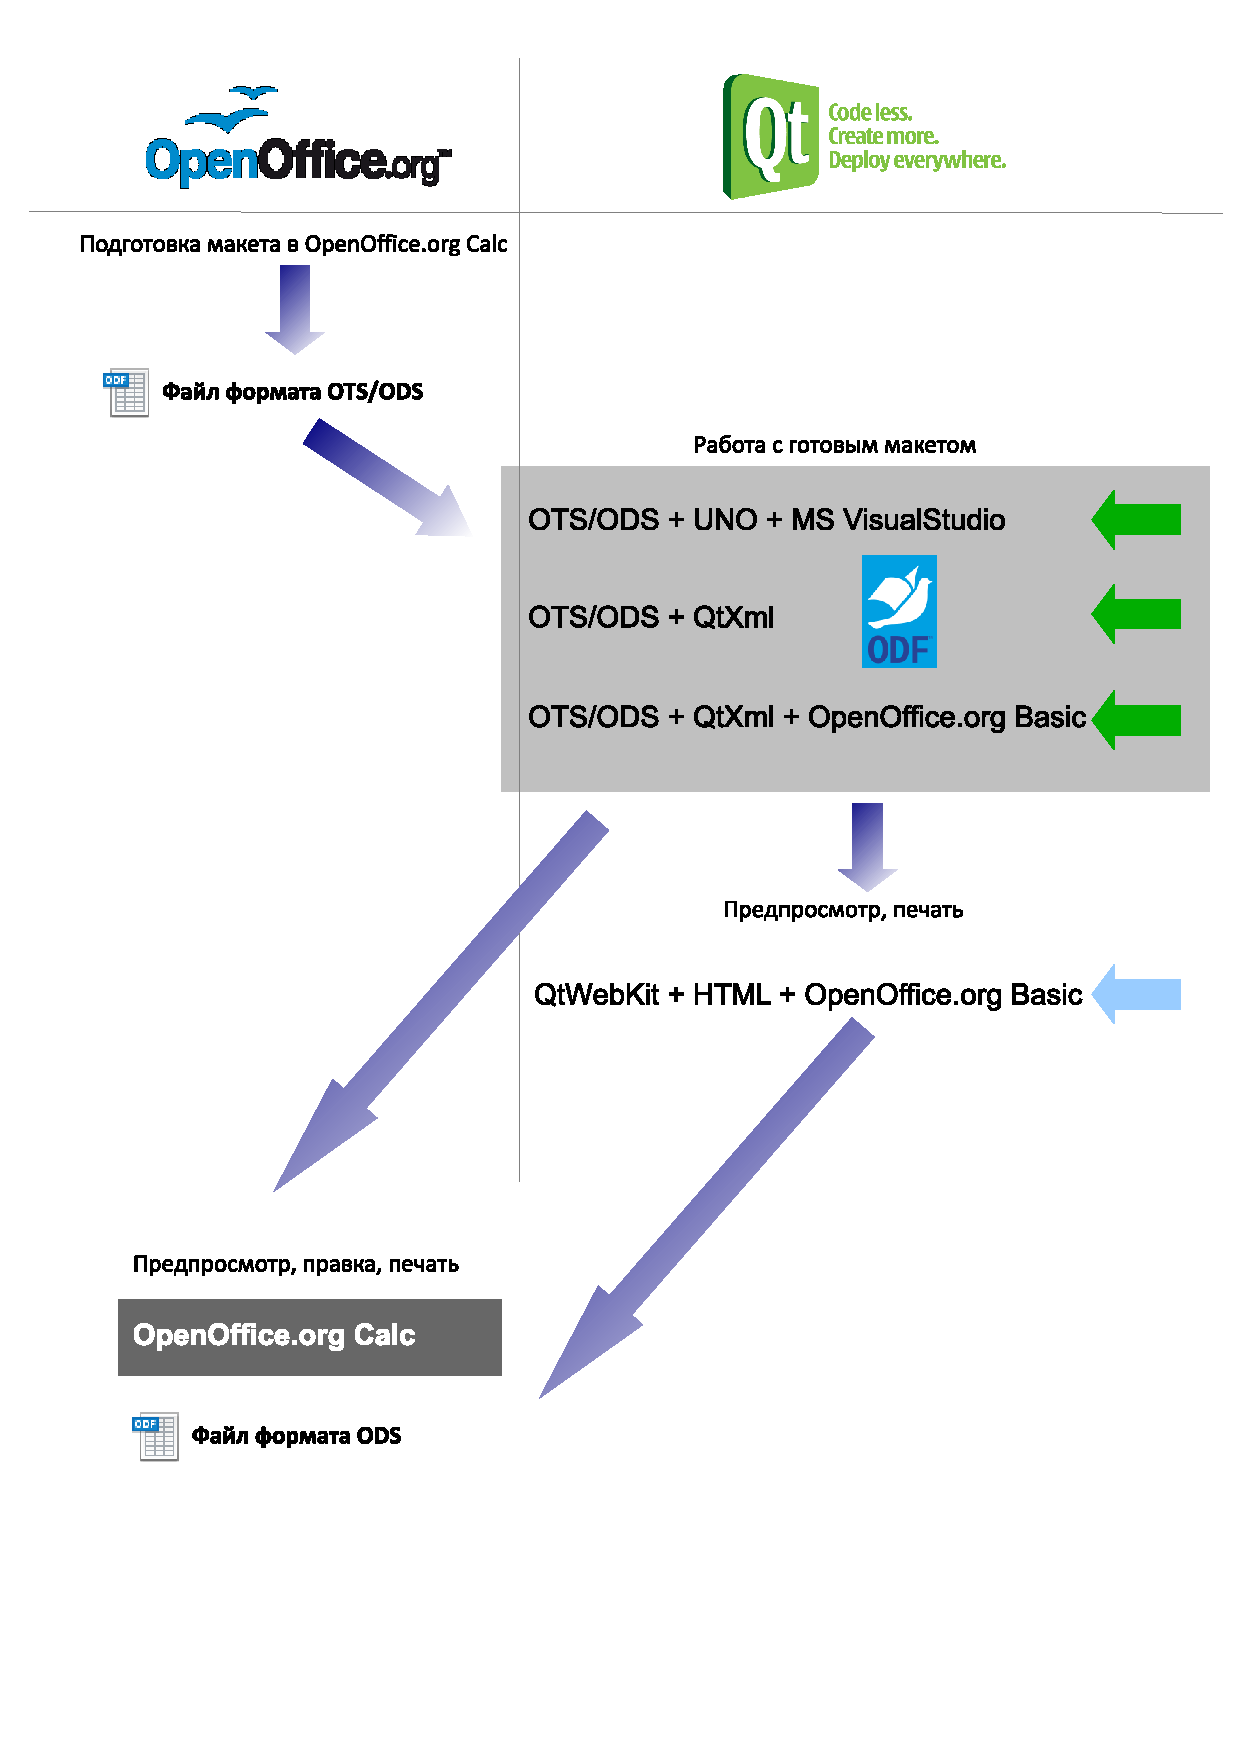
\includegraphics[height=0.6\textheight]{08_garanin}}
\end{figure}

\end{document}

\documentclass[10pt, a5paper]{article}
\usepackage{pdfpages}
\usepackage{parallel}
\usepackage[T2A]{fontenc}
\usepackage{ucs}
\usepackage[utf8x]{inputenc}
\usepackage[polish,english,russian]{babel}
\usepackage{hyperref}
\usepackage{rotating}
\usepackage[inner=2cm,top=1.8cm,outer=2cm,bottom=2.3cm,nohead]{geometry}
\usepackage{listings}
\usepackage{graphicx}
\usepackage{wrapfig}
\usepackage{longtable}
\usepackage{indentfirst}
\usepackage{array}
\newcolumntype{P}[1]{>{\raggedright\arraybackslash}p{#1}}
\frenchspacing
\usepackage{fixltx2e} %text sub- and superscripts
\usepackage{icomma} % коскі ў матэматычным рэжыме
\PreloadUnicodePage{4}

\newcommand{\longpage}{\enlargethispage{\baselineskip}}
\newcommand{\shortpage}{\enlargethispage{-\baselineskip}}

\def\switchlang#1{\expandafter\csname switchlang#1\endcsname}
\def\switchlangbe{
\let\saverefname=\refname%
\def\refname{Літаратура}%
\def\figurename{Іл.}%
}
\def\switchlangen{
\let\saverefname=\refname%
\def\refname{References}%
\def\figurename{Fig.}%
}
\def\switchlangru{
\let\saverefname=\refname%
\let\savefigurename=\figurename%
\def\refname{Литература}%
\def\figurename{Рис.}%
}

\hyphenation{admi-ni-stra-tive}
\hyphenation{ex-pe-ri-ence}
\hyphenation{fle-xi-bi-li-ty}
\hyphenation{Py-thon}
\hyphenation{ma-the-ma-ti-cal}
\hyphenation{re-ported}
\hyphenation{imp-le-menta-tions}
\hyphenation{pro-vides}
\hyphenation{en-gi-neering}
\hyphenation{com-pa-ti-bi-li-ty}
\hyphenation{im-pos-sible}
\hyphenation{desk-top}
\hyphenation{elec-tro-nic}
\hyphenation{com-pa-ny}
\hyphenation{de-ve-lop-ment}
\hyphenation{de-ve-loping}
\hyphenation{de-ve-lop}
\hyphenation{da-ta-ba-se}
\hyphenation{plat-forms}
\hyphenation{or-ga-ni-za-tion}
\hyphenation{pro-gramming}
\hyphenation{in-stru-ments}
\hyphenation{Li-nux}
\hyphenation{sour-ce}
\hyphenation{en-vi-ron-ment}
\hyphenation{Te-le-pathy}
\hyphenation{Li-nux-ov-ka}
\hyphenation{Open-BSD}
\hyphenation{Free-BSD}
\hyphenation{men-ti-on-ed}
\hyphenation{app-li-ca-tion}

\def\progref!#1!{\texttt{#1}}
\renewcommand{\arraystretch}{2} %Іначай формулы ў матрыцы зліпаюцца з лініямі
\usepackage{array}

\def\interview #1 (#2), #3, #4, #5\par{

\section[#1, #3, #4]{#1 -- #3, #4}
\def\qname{LVEE}
\def\aname{#1}
\def\q ##1\par{{\noindent \bf \qname: ##1 }\par}
\def\a{{\noindent \bf \aname: } \def\qname{L}\def\aname{#2}}
}

\def\interview* #1 (#2), #3, #4, #5\par{

\section*{#1\\{\small\rm #3, #4. #5}}

\def\qname{LVEE}
\def\aname{#1}
\def\q ##1\par{{\noindent \bf \qname: ##1 }\par}
\def\a{{\noindent \bf \aname: } \def\qname{L}\def\aname{#2}}
}


\begin{document}

\title{Базовая серверная архитектура для высоконагруженного стартапа}

\author{Михаил Пянко\\
\small Минск, ООО Анакреон,\texttt{mihail.pianko@warecorp.com}
}
\maketitle

\begin{abstract}
This article describes how to create a good environment for start-up project: what kind of server do we need for each role, and how these servers should communicate. Architecture restrictions are considered. Technical and architecture suggestions are made.
\end{abstract}

На начальном этапе разработки стартапа многие разработчики сталкиваются с проблемой создания достаточно гибкой и в будущем масштабируемой архитектуры приложения, оптимизированной для большой нагрузки. Мы хотели бы поделиться опытом в этой области. В качестве примера рассмотрим методы построения ресурса, базирующегося на Ruby On Rails. Тем не менее примеры, которые будут приведены ниже, с легкостью могут быть использованы для LAMP-решений. 

\section*{Серверы можно разделить на несколько типов по ролям:}
\begin{itemize}
\item Application
\item Database 
\item Load Balancer
\item Utils
\item Tools
\end{itemize}

{\bf Application} --- это frontend-сервер. Возможно использование как одного, так и нескольких Application-серверов. В случае использования одного Application-сервера надобности в балансировке нагрузки нет.

Application сервер выполняет следующие функции:
\begin{itemize}
\item обработка запросов от пользователей (получает запросы от балансировщика нагрузки),
\item взаимодействие с базой данных (Database server),
\item отправка сообщений в очередь сообщений (Utils server),
\item взаимодействие с CDN,
\item взаимодействие с search engines (Util server),
\item инвалидация кэша,
\item работа с кэшем (Database server).
\end{itemize}

Application сервер не должен производить следующих действий:
\begin{itemize}
\item преобразование медиа контента (видео, аудио, слайдшоу, и т.д.),
\item преобразование/кропинг картинок (если позволяет архитектура),
\item отправка сообщений электронной почты (если позволяет архитектура),
\item запросы на сторонние ресурсы через RestClient, curl, etc. (если позволяет архитектура).
\end{itemize}
{\bf Database} --- сервер, на котором находится база данных. В некоторых случаях на Database-сервер также устанавливается memcached, но это зависит от загрузки и конфигурации Database-сервера. 

Database-сервер выполняет следующие функции:
\begin{itemize}
\item обработка запросов от Application и Utils серверов,
\item хранение кэша (в случае установки memcached на DB сервер).
\end{itemize}
{\bf Load Balancer} --- балансировщик нагрузки, необходимый для распределения запросов пользователей между Application-серверами. Простейшим решением является использование nginx в качестве балансировщика нагрузки.

Load Balancer выполняет следующие функции:
\begin{itemize}
\item распределение запросов между Application серверами,
\item обработка HTTPS соединений (SSL сертификат должен быть сконфигурирован на балансировщике),
\item кэширование при использовании Varnish или связки nginx + memcache,
\item Firewall.
\end{itemize}

{\bf Utils} --- сервер, на котором располагаются сопутствующие сервисы, необходимые для отложенной обработки данных. Вот краткий список:
\begin{itemize}
\item message queue (RabbitMQ, Apache Message Queue, etc),
\item search engines (Solr, Sphinx, etc),
\item обработчики сообщений,
\item сервисы для обработки Video, Audio, SlideShow,
\item отправка сообщений электронной почты,
\item взаимодействие с CDN,
\item инвалидация кэша,
\item взаимодействие со сторонними ресурсами (PDF converters, \linebreak SendGrid, etc.). 
\end{itemize}
{\bf Tools} "--- сервер, необходимый для установки сторонних решений для работы приложения. В частности, приложения, базирующиеся на Java/Tomcat, система мониторинга и ресурсы, в безопасности которых вы сомневаетесь (Spellchecker, etc.). Tools-сервер не может установить соединения с Application, Database, Utils-серверами. Единственный протокол взаимодействия "--- это HTTP. Это дает гарантию того, что в результате взлома стороннего компонента основная ферма не пострадает. Сервер с этой ролью не обязателен. 


\begin{figure}[ht]
\centering{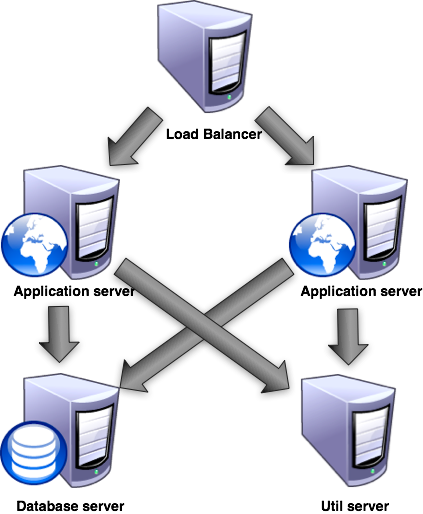
\includegraphics[width=8cm]{09_pianko.png}}
\label{pic:fl1}
%\caption{~}
\end{figure}

\section*{Ограничения, которые накладываются на архитектуру приложения}

\subsection*{Хранение кэша}
Необходимо организовать централизованное хранилище кэша. Файловый кэш и кэширование данных в памяти сервера работать не будет, так как кэш может создаваться и инвалидироваться с разных серверов. Наилучшим решением в данном случае является использования memcached. 

\subsection*{Хранение сессий пользователя}
В данном случае целесообразно хранить сессии в memcached или в Cookies. Отдача сессии на сторону пользователя --- менее безопасное и более медленное решение, чем хранение в memcached. 

\subsection*{Хранение медиа-данных пользователя}
Любой контент, загруженный пользователем на сервер, не может быть просто  сохранен в папку /public/upload. Наилучшим способом хранения данных является CDN. 

\subsection*{Рекомендации по автоматизированной конфигурации серверов}
Существует достаточно большое количество ПО для поддержания конфигурации серверов: Сfengine, Puppet, Chef, Sprinkle. 

Для автоматизированного конфигурирования серверов мы используем Sprinkle. Sprinkle --- это достаточно простое приложение на RoR, позволяющее разрабатывать сценарии по установке ПО на UNIX"=сервера.  Sprinkle поддерживает разделение серверов на роли, фермы и т.д. Так же поддерживаются различные типы инсталяторов, методов проверки текущей конфигурации, источников данных. Sprinkle имеет открытый исходный код, что позволяет вносить изменения в логику работы отдельных компонентов или создавать дополнительные модули. 

\section*{Варианты инсталляции}
Существует несколько вариантов ферм.
\begin{itemize}
\item Single server installation.
  \begin{itemize}
  \item На одном сервере располагаются Application + Util + Database
  \end{itemize}
\item Light farm
  \begin{itemize}
  \item $1$ сервер: Application 
  \item $1$ сервер: Util + DB
  \end{itemize}
\item Big farm:
  \begin{itemize}
  \item $1$ сервер: Load Ballancer 
  \item $x$ серверов: Application
  \item $1-x$ серверов: Util 
  \item $1-x$ серверов: Database (о репликациях и масштабировании базы данных можем поговорить чуть позже) 
  \end{itemize}
\end{itemize}
На самом деле существует множество комбинаций распределения ролей по физическим серверам. Необходимо выбирать оптимальный вариант в зависимости от нагрузки на сервера каждой роли. 

\section*{Рекомендации по архитектуре. Несколько примеров}

\subsection*{Интеграция со сторонними ресурсами}
Зачастую необходима интеграция со сторонними ресурсами для преобразования видео и аудио, обработки слайд-шоу, отсылки писем и т.д. 

Это подразумевает установку соединения по протоколам TCP, HTTP, etc. 
В данном случае существует несколько рисков:
\begin{itemize}
\item сервер недоступен
\item сервер перегружен 
\end{itemize}

В первом случае пользователь не сможет завершить действие, часть данных может быть потеряна или пользователь увидит сообщение ошибки на экране. 
Во втором случае мы получим очень долгую обработку страницы, что доставит неудобство пользователю. 

Лучшим решением в данном случае является отправка события в очередь сообщений и обработка на стороне util"=сервера. 

\subsection*{Обработка картинок пользователя}
Если ваш ресурс поддерживает возможность загрузки аватаров пользователей, логотипов с последующим ресайзингом изображений, вы можете столкнуться с проблемой большой нагрузки на сервер. 

Есть несколько распространенных методов ресайзинга изображений:

\begin{itemize}
\item оригинальное изображение сохраняется в хранилище без обработки. Доступ к изображению со страниц сайта реализован через врапер с элементарной логикой. Если картинка сгенерирована, то необходимо отдать ее через STDOUT или вернуть редирект на статический. Если картинка отсутствует, то сгенерировать и выполнить предыдущий шаг. Проблема этого метода в том, что нагрузка, которую может создать данный алгоритм, не может быть спрогнозирована.  При добавлении нового размера изображения достаточно визита поискового бота - и скорее всего сервера будут перегружены. 
\item оригинальное изображение преобразуется в нужные форматы и размеры непосредственно после загрузки на сервер. Это дает единовременную нагрузку на Application-сервера. Минусом данного метода является задержка в возврате страницы пользователю, что может вызвать дискомфорт.
\item последний вариант является модифицированной версией \linebreak предыдущего. Вместо непосредственной обработки изображения на Application-сервере необходимо отправить событие в очередь сообщения и произвести обработку изображения на Util"=сервере. 
\end{itemize}

\section*{Заключение}

Выше приведены приемы для построения начальной архитектуры высоконагруженной системы, которая в будущем может быть легко расширена и  смасштабирована. Способы дальнейшего развития напрямую зависят от архитектуры приложения, нагрузки на отдельные узлы системы и специфики проекта.

\end{document}





\documentclass[10pt, a5paper]{article}
\usepackage{pdfpages}
\usepackage{parallel}
\usepackage[T2A]{fontenc}
\usepackage{ucs}
\usepackage[utf8x]{inputenc}
\usepackage[polish,english,russian]{babel}
\usepackage{hyperref}
\usepackage{rotating}
\usepackage[inner=2cm,top=1.8cm,outer=2cm,bottom=2.3cm,nohead]{geometry}
\usepackage{listings}
\usepackage{graphicx}
\usepackage{wrapfig}
\usepackage{longtable}
\usepackage{indentfirst}
\usepackage{array}
\newcolumntype{P}[1]{>{\raggedright\arraybackslash}p{#1}}
\frenchspacing
\usepackage{fixltx2e} %text sub- and superscripts
\usepackage{icomma} % коскі ў матэматычным рэжыме
\PreloadUnicodePage{4}

\newcommand{\longpage}{\enlargethispage{\baselineskip}}
\newcommand{\shortpage}{\enlargethispage{-\baselineskip}}

\def\switchlang#1{\expandafter\csname switchlang#1\endcsname}
\def\switchlangbe{
\let\saverefname=\refname%
\def\refname{Літаратура}%
\def\figurename{Іл.}%
}
\def\switchlangen{
\let\saverefname=\refname%
\def\refname{References}%
\def\figurename{Fig.}%
}
\def\switchlangru{
\let\saverefname=\refname%
\let\savefigurename=\figurename%
\def\refname{Литература}%
\def\figurename{Рис.}%
}

\hyphenation{admi-ni-stra-tive}
\hyphenation{ex-pe-ri-ence}
\hyphenation{fle-xi-bi-li-ty}
\hyphenation{Py-thon}
\hyphenation{ma-the-ma-ti-cal}
\hyphenation{re-ported}
\hyphenation{imp-le-menta-tions}
\hyphenation{pro-vides}
\hyphenation{en-gi-neering}
\hyphenation{com-pa-ti-bi-li-ty}
\hyphenation{im-pos-sible}
\hyphenation{desk-top}
\hyphenation{elec-tro-nic}
\hyphenation{com-pa-ny}
\hyphenation{de-ve-lop-ment}
\hyphenation{de-ve-loping}
\hyphenation{de-ve-lop}
\hyphenation{da-ta-ba-se}
\hyphenation{plat-forms}
\hyphenation{or-ga-ni-za-tion}
\hyphenation{pro-gramming}
\hyphenation{in-stru-ments}
\hyphenation{Li-nux}
\hyphenation{sour-ce}
\hyphenation{en-vi-ron-ment}
\hyphenation{Te-le-pathy}
\hyphenation{Li-nux-ov-ka}
\hyphenation{Open-BSD}
\hyphenation{Free-BSD}
\hyphenation{men-ti-on-ed}
\hyphenation{app-li-ca-tion}

\def\progref!#1!{\texttt{#1}}
\renewcommand{\arraystretch}{2} %Іначай формулы ў матрыцы зліпаюцца з лініямі
\usepackage{array}

\def\interview #1 (#2), #3, #4, #5\par{

\section[#1, #3, #4]{#1 -- #3, #4}
\def\qname{LVEE}
\def\aname{#1}
\def\q ##1\par{{\noindent \bf \qname: ##1 }\par}
\def\a{{\noindent \bf \aname: } \def\qname{L}\def\aname{#2}}
}

\def\interview* #1 (#2), #3, #4, #5\par{

\section*{#1\\{\small\rm #3, #4. #5}}

\def\qname{LVEE}
\def\aname{#1}
\def\q ##1\par{{\noindent \bf \qname: ##1 }\par}
\def\a{{\noindent \bf \aname: } \def\qname{L}\def\aname{#2}}
}


\begin{document}
\title{Мониторинг Linux/FreeBSD серверов}
\author{Николай Маржан\footnote{Киев, Украина, PortaOne, Inc. \url{delgod@delgod.com}}}

\maketitle



\begin{abstract}Purposes and functions of monitoring systems are discussed, as far as general approaches to analyze the diagnostic parameters of a server. Observed information is classified into parameters received from hardware maintenance, operating system, services and typical database. Sample diagnostic parameters are presented for each category.
\end{abstract}

К стандартным целям проводимого на серверах мониторинга можно отнести:
\begin{itemize}
	\item Отслеживание критических значений диагностических параметров состояния и уведомление инженеров об их появлении.
	\item Накопление статистической информации для последующего анализа.
\end{itemize}

Уведомление о том, что система находится в критическом состоянии, является наиболее важной функцией мониторинга, так как требует немедленного вмешательства инженеров, которые занимаются поддержкой данной системы.

Даже если проблема носит временный характер (например, стопроцентная загрузка процессора, возникшая спонтанно и затем прекратившаяся через 20 минут), выяснить причину такого поведения можно только тогда, когда проблема присутствует (причиной могла быть удаленная DOS-атака).

Накопление статистической информации происходит обычно в 2-х видах:
\begin{itemize}
	\item Лог-файлы. Обычно в них записываются только те моменты, когда система входит в критическое состояние, и когда возващается в нормальное.
	\item Данные для графиков по каждому показателю.
\end{itemize}

Графики --- не менее важная часть системы мониторинга, так как только они позволяют проводить анализ состояния сервера в целом, как сложной системы. 
Используя графики для наблюдения динамики диагностических параметров, мы можем:
\begin{itemize}
	\item Увидеть, в каком состоянии находился сервер в любой момент времени в прошлом. Мы можем быстро понять, чем отличается сегодняшнее состояние от состояния недельной давности.
	\item Проследить закономерности возможной взаимосвязи между диагностическими параметрами. Например, когда повышается входящий трафик на сетевом интерфейсе --- повышается нагрузка на центральный процессор.
	\item Находить противоречия между значениями диагностических параметров. Например, сильно возросло количество запросов на чтение к базе данных, и база данных начала использовать на 1 Гб больше оперативной памяти, но при этом с жесткого диска было считано всего 100 Мб данных.
 Увидеть, в каком состоянии находился сервер в любой момент времени в прошлом. Мы можем быстро понять, чем отличается сегодняшнее состояние от состояния недельной давности.
	\item Проследить закономерности возможной взаимосвязи между диагностическими параметрами. Например, когда повышается входящий трафик на сетевом интерфейсе --- повышается нагрузка на центральный процессор.
	\item Находить противоречия между значениями диагностических параметров. Например, сильно возросло количество запросов на чтение к базе данных, и база данных начала использовать на 1 Гб больше оперативной памяти, но при этом с жесткого диска было считано всего 100 Мб данных.
\end{itemize}
Диагностическими параметрами состояния для аппаратного обеспечения являются: 
\begin{enumerate}
	\item температура центрального процессора;
	\item наличие повреждённых секторов или ошибок чтения на жестком диске;
	\item состояние аппаратного RAID-контроллера.
\end{enumerate}
К диагностическим параметрам состояния для операционной системы можно отнести:
\begin{enumerate}
	\item количество задач, ожидающих выполнения (load average);
	\item время простоя центрального процессора (idle);
	\item время простоя каждого ядра центрального процессора (idle);
	\item размер свободного места на жестком диске;
	\item нагрузка на жесткий диск;
	\item количество данных в разделе подкачки (swap);
	\item активная запись или чтение с раздела подкачки (swaping/paging);
	\item количество использованной памяти;
	\item количество памяти, потребляемой каждым приложением;
	\item скорость передачи данных на сетевых интерфейсах;
	\item подтверждение того, что сетевые интерфейсы работают на нужной скорости и в полнодуплексном режиме;
	\item количество ошибок и коллизий на сетевых интерфейсах;
	\item состояние системных буферов (freebsd vm.zone), mbuf clusters, sendfile-буферов, размер KVM, Pipe KVA;
	\item количество открытых файлов, количество открытых сокетов;
	\item отсутствие процессов-зомби;
	\item отсутствие ошибок сегментации у процессов.
\end{enumerate}
Диагностическими параметрами состояния сервисов являются:
\begin{enumerate}
	\item подтверждение того, что все критически важные сервисы запущены.
	\item подтверждение того, что сервисы успевают вычитывать данные из входящей очереди сетевой подсистемы.
	\item подтверждение того, что нет отброшенных данных вследствие полных буферов соединения (dropped due to full socket buffers).
\end{enumerate}
Диагностическими параметрами состояния базы данных MySQL являются:
\begin{enumerate}
	\item количество максимально использованных соединений;
	\item количество запросов, количество медленных запросов;
	\item количество операций записи/чтения с жесткого диска;
	\item отставание репликации.
\end{enumerate}
Как показал опыт построения систем мониторинга в гетерогенных сетях, подходы и диагностические параметры практически идентичны для операционных систем FreeBSD и Linux; основные различия связаны с мониторингом системных буферов и с некоторыми расхождениями в синтаксисе команд.
\end{document}

\documentclass[10pt, a5paper]{article}
\usepackage{ucs}
\usepackage[utf8]{inputenc}
\usepackage[T2A]{fontenc}
\usepackage[english, russian]{babel}
\usepackage{hyperref}
\usepackage{geometry}
\frenchspacing
\begin{document}
\title{Darktable, приложение для каталогизации и обработки RAW-файлов}
\author{Константин Шевцов\footnote{Новополоцк/Минск, Беларусь, \url{kanstantsin.sha@gmail.com}}, Александр Рабцевич\footnote{Минск, Беларусь, \url{alexander.v.rabtchevich@gmx.net}}}
\date{}

\def\progref!#1!{\texttt{#1}}

\maketitle

\begin{abstract}
Darktable is an open source application devoted to processing of RAW files. The program can manage collections of RAWs with rating, color labels and custom tags. A rich set of build-in filters (some of them are unique), used at processing, store their settings in a form of a history stack, which is saved alongside original RAW, providing original RAW untouched. Due to rawspeed RAW importing library, multi-threading and permanent optimizations, the program is fast and responsive.
\end{abstract}

\section*{История}
В докладе описывается история появления и развития проекта, возможности программы на примере работы с RAW файлами, а также планы разработчиков по развитию программы.

До появления darktable в ОС Linux отсутствовал открытый инструмент, сочетающий возможности каталогизации коллекции RAW файлов с их неразрушающей обработкой. UFRaw и  Rawtherapee не обладают достаточными возможностями для профессионального фотографа.

Восполнить пробел решил Йоханес Ханика (Johannes Hanika), который зарегистрировал проект darktable на SourceForge в феврале 2009 года. Вскоре к нему присоединились 3 разработчика: Хенрик Андерсон (Henrik Andersson), Паскаль де Брайн (Pascal de Bruijn), Александр Прокудин. В настоящее время у проекта около 20 контрибьюторов. 

\section*{Описание}
Спиосок основных возможностей программы при работе с коллекцией включает:
\begin{itemize}
\item импорт фотографий в коллекцию из папки, импорт отдельных фотографий. Фотографии физически не перемещаются.
\item импорт из фотоаппарата посредством gPhoto2
\item хранение данных о коллекции в собственной базе данных
присвоение фотографиям рейтинга (stars), система цветовых меток, пользовательские теги (метки).
\item поиск по произвольной комбинации: съемка, камера, метка, дата, наличие изменений после экспорта.
\item копирование истории обработки между фотографиями
\item экспорт в jpeg, tiff (8 и 16 бит) 
\item экспорт в picasa, flickr, email
Основные возможности программы по обработке RAW (версия из репозитария git):
\item внутреннее представление данных RGB float (32 бит/канал) или LCh (в зависимости от модуля)
\item быстрый предосмотр с масштабированием вплоть до 100\%, при предосмотре обрабатывается только часть изображения, показываемая в окне с кешированием операций
\item многопоточность
\item использование для ряда операций OpenCL при наличии драйвера и подходящего графического ускорителя
\item все изменения хранятся в виде стека истории с возможностью отката до произвольной точки, а также копирования истории изменений между фотографиями или сохранения ее в виде стиля для последующего применения
\item стек истории сохраняется в виде *.xmp файла вместе с оригинальным файлом RAW
\item модульная архитектура (плагины)
\item возможность создания и ручного/автоматического использования предустановок для всех модулей
\item наличие режимов смешивания для большинства модулей
\item алгоритмы дебайеризации ppg и AMaZE 
\item поканальный баланс белого через множители либо через  - сдвиг цветовой температуры и множителя зеленого канала
\item редактируемая тональная кривая камеры с возможностью выбора из набора готовых кривых, аналогичных используемым производителями цифровых фотоаппаратов
\item восстановление пересветов при отрицательной экспокоррекции
\item профили камеры: стандартные (Adobe), улучшенные, либо пользовательские
\item трансформации: кадрирование с выбираемым соотношением сторон, поворот, перспектива
\item редактируемая тональная кривая (L канал в LCh пространстве
\item возможность работать с тональной кривой в виде последовательности зон Адамса
\item мощнейший инструмент --- эквалайзер, позволяющий регулировать локальный контраст (L и С) в зависимости от пространственной частоты (аналога радиуса в USM) с помощью избегающих краев вейвлетов
\item подавление шума
\item исправление геометрических искажений оптики с помощью библиотеки lensfun
\item регулирование яркости/насыщенности или сдвига тонов в плагине цветовые зоны
\item микшер каналов
\item обесцвечивание с регулируемым цветовым фильтром
\item градиентный фильтр (GND) с возможностью поворота и радиального смещения
\item эффект виньетирования с регулируемыми на холсте радиусом, формой (окружность/эллипс)
\item вельвия
\item смягчающий фильтр
\item и другие фильтры
\end{itemize}

\section*{Будущее}
В настоящее время разработчики готовят программу к выпуску версии 0.9. 

В ближайших планах разработчиков --- добавление функционала масок (Henrik Andersson) и переработка интерфейса с централизованной обработкой горячих клавиш (GSoC студент Robert Bieber). В состоянии обсуждения — возможность не  однократного использования плагинов. В более отдаленных планах — использование GEGL внутри darktable с возможностью передачи данных в GIMP и обратно для более сложного редактирования; однако этот функционал может появиться не раньше выхода GIMP 3.0.

Проект активно развивается и радует постоянное растущее сообщество пользователей новыми выпусками с периодичностью примерно раз в три месяца. Можно ответственно заявить, что текущая версия пригодна для использования профессиональным фотографом.

\begin{thebibliography}{9}
\bibitem{pDynamo} Официальный сайт проекта --- \url{http://darktable.sf.net}
\end{thebibliography}
\end{document}

\documentclass[10pt, a5paper]{article}
\usepackage{ucs}
\usepackage[utf8]{inputenc}
\usepackage[T2A]{fontenc}
\usepackage[english, russian]{babel}
\usepackage{hyperref}
\usepackage{geometry}
\frenchspacing

\begin{document}

\title{On Digital Monies}

\author{Daniel Nagy\footnote{Budapest, Hungary, ePoint Systems Ltd., \url{nagydani@epointsystem.org}}}
\date{}
\maketitle
\renewcommand{\abstractname}{Abstract}
\begin{abstract}
Payment over digital communications networks has been a hot topic since
the introduction of the telegraph, the first such electronic network;
originally, Western Union was a telegraph company. Money, however, is
more than a means of payment: it is also an instrument of saving and
credit, a measure of value and a unit of accounting. In my presentation,
I shall explore various attempts at creating digital money, both
proprietary and open-source, theoretical and practical.
\end{abstract}

The main difference between digitally represented information and
everything else that has been historically used as money is that unlike
the latter, digital information can be copied at no cost, with perfect
fidelity in essentially unlimited quantities. Very undesirable
properties for something that we intend to use as money. This is the
main technical challenge in using digital information as money (known as
``double spending''). How can we make sure that no more gets spent than
what has been earned?

There is, however, a different, no less interesting challenge that is
not purely technical: how to get actual people provide real value in
exchange for pieces of digital information. Why would people use pieces
of digital information as a means of exchange or to keep their savings
or to measure value?

The third challenge is a legal one. Since the first ever gold coins have
been minted at the behest of Croesus, King of Lydia in the sixth
century, B.C., money has been subject of government regulation and very
often exclusive monopoly. How can digital money exist within the current
legal framework?

Different solutions to these challenges have been proposed. We shall
explore the solutions to these challenges in the following systems in
some technical detail:

\subsubsection*{DigiCash}
David Chaum's company founded in 1990 on the basis of some clever
cryptography -- blind digital signatures -- he published in 1988. The
company declared bankruptcy in 1998, but in many ways it provided
inspiration to the many ventures that followed. I brief and simplified
introduction to the technology will be given as well as what I think
were the reasons for failure.

\subsubsection*{WebMoney}
Artiom Genkin went the other route: his doctoral thesis on the topic
followed business success. Founded in 1998, WebMoney made its name by
proving to be more resilient in the face of financial meltdown than the
Russian banking sector. To this day, WebMoney is one of the most
sophisticated and successful digital money, albeit mostly in the
Russian-speaking world.

\subsubsection*{BitCoin}
This is an open-source project started in 2009 by the mysterious Satoshi
Nakatomo, based on earlier research either done or popularized by Nick
Szabo (a former DigiCash employee). This year, BitCoin's popularity (and
valuation) exploded, making it one of the most important and interesting
innovations in the field.

\subsubsection*{ePoint}
This is my own open-source project, kicked off in 2005. However, I am
not going to talk much about how it works now; rather, I shall outline
where I would like to take it and what needs to be done to get there.
Maybe, I like-minded developers of open-source software among LVEE 2011
participants will join me in creating something valuable and useful.


\end{document}





\documentclass[10pt, a5paper]{article}
\usepackage{ucs}
\usepackage[utf8]{inputenc}
\usepackage[T2A]{fontenc}
\usepackage[english, russian]{babel}
\usepackage{hyperref}
\usepackage{geometry}
\usepackage{graphicx}
\frenchspacing

\begin{document}

\title{Linux и СПО в создании музыки и живом исполнении. Обзор имеющихся программ и ниши применения}
\author{Сергей Васильев\footnote{Таллинн, Эстония, \url{zyxos2@gmail.com}}}
\date{}
\maketitle
\begin{abstract}
The aspects of using Linuz and free software in amateur music creation, sound editing and live performances are reviewed.
\end{abstract}

Ещё несколько лет назад Linux был малопригоден для работы со звуком; за последние годы ситуация значительно изменилась: улучшилась поддержка многих звуковых карт, MIDI-контроллеров и MIDI-интерфейсов, появились новые программы, интерфейс которых изменился в лучшую сторону, что снизило порог вхождения для начинающих пользоваталей. И, несмотря на некоторые всё ещё присутствующие проблемы, сейчас вполне возможно использование решений на базе Linux и СПО в любительской музыкальной деятельности. Применение данных решений имеет ряд преимуществ, одним из которых является низкая стоимость, что немаловажно для начинающих музыкантов. 

Многие начинающие музыканты не обращают внимания на Linux из-за недостаточной информированности, и очень часто для выполнения простых задач прибегают к применению программного обеспечения, возможности которого на порядок превышают потребности, что приводит к нерациональному расходу денежных средств или к незаконному использованию коммерческих приложений. Имеющейся на данный момент программной базы и поддержки оборудования достаточно для выполнения основных задач. 

В таблице приведены категории и некоторые программы, которые, после сравнительного анализа, были отобраны как наиболее подходящие для использования в сетапе для демонстрации.

\begin{figure}[ht]
\centering{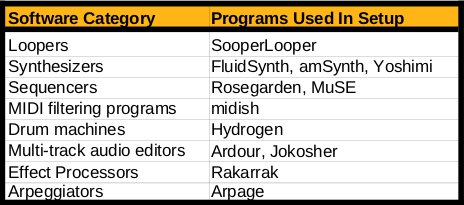
\includegraphics[width=8cm]{13_abstract.jpg}}
%\label{pic:fl1}
\caption{Приложения по категориям}
\end{figure}

По субъективной оценке, наиболее заполнены категории многодорожечных аудиоредакторов, представленных мощнейшим проектом Ardour, и некоторыми более простыми; процессоров эффектов --- Rakarrak и др.; также почти на 100\% покрывает потребности замечательный редактор табулатур TuxGuitar.

Драм-машины представлены практически одним проектом Hydrogen, но довольно мощным, лишь с небольшими пожеланиями усовершенствований в области мульти-лэйеринга.

Что касается луперов и арпеджиаторов --- лидеры SooperLooper и Arpage предоставляют базовую функциональность, но хотелось бы надеяться на улучшения в будущем.

Категории с некоторым количеством недочетов --- секвенсеры и MIDI-фильтры.

Проблемные категории --- синтезаторы (несмотря на замечательные программы FluidSynth, amSynth и Yoshimi, ситуация  c VST-плагинами все еще далека от идеальной) и автоаккомпаниаторы (поскольку MMA очень сильно нехватает адекватного GUI).
\end{document}

\documentclass[10pt, a5paper]{article}
\usepackage{pdfpages}
\usepackage{parallel}
\usepackage[T2A]{fontenc}
\usepackage{ucs}
\usepackage[utf8x]{inputenc}
\usepackage[polish,english,russian]{babel}
\usepackage{hyperref}
\usepackage{rotating}
\usepackage[inner=2cm,top=1.8cm,outer=2cm,bottom=2.3cm,nohead]{geometry}
\usepackage{listings}
\usepackage{graphicx}
\usepackage{wrapfig}
\usepackage{longtable}
\usepackage{indentfirst}
\usepackage{array}
\newcolumntype{P}[1]{>{\raggedright\arraybackslash}p{#1}}
\frenchspacing
\usepackage{fixltx2e} %text sub- and superscripts
\usepackage{icomma} % коскі ў матэматычным рэжыме
\PreloadUnicodePage{4}

\newcommand{\longpage}{\enlargethispage{\baselineskip}}
\newcommand{\shortpage}{\enlargethispage{-\baselineskip}}

\def\switchlang#1{\expandafter\csname switchlang#1\endcsname}
\def\switchlangbe{
\let\saverefname=\refname%
\def\refname{Літаратура}%
\def\figurename{Іл.}%
}
\def\switchlangen{
\let\saverefname=\refname%
\def\refname{References}%
\def\figurename{Fig.}%
}
\def\switchlangru{
\let\saverefname=\refname%
\let\savefigurename=\figurename%
\def\refname{Литература}%
\def\figurename{Рис.}%
}

\hyphenation{admi-ni-stra-tive}
\hyphenation{ex-pe-ri-ence}
\hyphenation{fle-xi-bi-li-ty}
\hyphenation{Py-thon}
\hyphenation{ma-the-ma-ti-cal}
\hyphenation{re-ported}
\hyphenation{imp-le-menta-tions}
\hyphenation{pro-vides}
\hyphenation{en-gi-neering}
\hyphenation{com-pa-ti-bi-li-ty}
\hyphenation{im-pos-sible}
\hyphenation{desk-top}
\hyphenation{elec-tro-nic}
\hyphenation{com-pa-ny}
\hyphenation{de-ve-lop-ment}
\hyphenation{de-ve-loping}
\hyphenation{de-ve-lop}
\hyphenation{da-ta-ba-se}
\hyphenation{plat-forms}
\hyphenation{or-ga-ni-za-tion}
\hyphenation{pro-gramming}
\hyphenation{in-stru-ments}
\hyphenation{Li-nux}
\hyphenation{sour-ce}
\hyphenation{en-vi-ron-ment}
\hyphenation{Te-le-pathy}
\hyphenation{Li-nux-ov-ka}
\hyphenation{Open-BSD}
\hyphenation{Free-BSD}
\hyphenation{men-ti-on-ed}
\hyphenation{app-li-ca-tion}

\def\progref!#1!{\texttt{#1}}
\renewcommand{\arraystretch}{2} %Іначай формулы ў матрыцы зліпаюцца з лініямі
\usepackage{array}

\def\interview #1 (#2), #3, #4, #5\par{

\section[#1, #3, #4]{#1 -- #3, #4}
\def\qname{LVEE}
\def\aname{#1}
\def\q ##1\par{{\noindent \bf \qname: ##1 }\par}
\def\a{{\noindent \bf \aname: } \def\qname{L}\def\aname{#2}}
}

\def\interview* #1 (#2), #3, #4, #5\par{

\section*{#1\\{\small\rm #3, #4. #5}}

\def\qname{LVEE}
\def\aname{#1}
\def\q ##1\par{{\noindent \bf \qname: ##1 }\par}
\def\a{{\noindent \bf \aname: } \def\qname{L}\def\aname{#2}}
}


\begin{document}

\title{Amazon auto-scaling. Создание и оптимизация автомасштабируемых систем на базе GNU/Linux}
\author{Виктор Краев\footnote{Минск, Беларусь, \url{anakreon.by}}}
\date{}
\maketitle
\begin{abstract}\noindent 
The technology of auto-scaling clasters provided by Amazon for its cloud services is reviewed. Approach to monitor and control such cloud-based system is presented, as far as practical expe\-ri\-ence of migrating to the auto-scaled services.
\end{abstract}

\section*{Amazon EC2. Cloud vs Hardware}
С каждым годом IT-индустрия набирает обороты, но как бы не развивались технологии, ресурс выработки железа пока никто не победил. Отказ оборудования по-прежнему является одной из главных проблем современного хостинга. Конечно же, всегда есть возможность создания избыточности, но это тянет за собой достаточно серьезные расходы на дополнительное оборудование и его обслуживание. Поэтому наша компания обратила внимание на облачные вычисления. Наиболее продвинутой компанией, способной решить наши задачи, на сегодняшний день оказалась Amazon. Хотя их технология Elastic Cloud --- местами сырая, она находится в активной разработке и интегрируется с другими сервисами, нивелирующими ее недостатки. Не победив проблему «железа», в Amazon создали избыточность, покрыв недостатки другими сервисами, и сегодня падение инстансов (instances) или потеря данных в облаке иногда присутствует, но успешно компенсируется резервным копированием и высокой скоростью создания инстансов из резервных копий. Интеграция с такими сервисами, как auto-scaling, cloudwatch, cloudformation, позволяет добиться избыточности, намного превышающей возможности обычного кластера серверов, не задумываясь о «железе».  

\section*{Amazon Auto-Scaling. Hardware cluster vs scalable cloud}

На сегодняшний день для увеличения доступности и избыточности ресурса используют технологии кластеризации. Статический кластер подразумевает под собой использование определенного неизменяемого количества (больше 1) серверов, нагрузку между которыми распределяет балансировщик (Load Balancer). Это хорошее решение для ресурсов с постоянно высокой нагрузкой. Динамический кластер --- это кластер, где распределение нагрузки осуществляется между серверами, количество которых может меняться в зависимости от нужд и нагруженности проекта. Однако в «железе» это трудноосуществимо, т.к. тянет за собой целый шлейф проблем, связанных с установкой оборудования, разворачиванием ПО, а главное --- времени. С помощью сервиса EC2 на создание виртуального сервера уходит несколько минут. Создание происходит из уже готового образа (image), т.~е. выполняется клонирование существующей системы. Обычно это образы «чистых» систем, в которых установлены лишь базовые пакеты. Но Amazon позволяет создавать собственные образы уже настроенных и готовых к использованию систем --- например, хостинговых. Полученные образы помещаются в приватное хранилище, из которого в любой момент можно создать и отправить в работу клон. Эта технология, лежащая в основе создания динамического кластера и известная как AMI, позволяет мгновенно создавать кластеры различного размера. Для распределения нагрузки между элементами кластера используется сервис ELB (Elastic Load Balancer), который позволяет менять размерность кластера путем добавления или удаления виртуальных серверов в балансировщик. Однако, используя лишь web-интерфейс, вы сможете управлять кластером только вручную. Это значит, что если один из элементов кластера откажет в обслуживании, то балансировщик выбросит его из пула обрабатываемых запросов, и новый виртуальный сервер не встанет на его место автоматически. Чтобы автоматизировать этот процесс в Amazon придумали технологию Auto-Scaling. Эта технология позволяет задавать размерность кластера и использует проверку здоровья (health cheacking) серверов из ELB или EC2. В случае падения на место упавшего сервера из образа автоматически создается новый сервер и добавляет его в балансировщик. Сегодня управление конфигурацией Auto-Scaling осуществляется только через API, что позволяет автоматизировать процессы создания кластеров и управления ими, убирая из цепочки слабое звено "--- человека.

\section*{Amazon CloudWatch. Monitor and automate your systems}

Мы можем не только управлять собственной армией виртуальных серверов, но и получать данные о ее работе. Технология \linebreak CloudWatch позволяет осуществлять мониторинг. В основе этой технологии лежат метрики (metrics) "--- данные, собираемые с инстансов и агрегируемые по различным критериям в группы. Нельзя сказать, что технология блещет богатством собираемых коллекций, хотя в ней присутствует мониторинг CPU, дисковой и сетевой подсистем, количества запросов в ELB и т.\,д. Но с помощью API вы можете собирать свою собственную коллекцию метрик, которую в дальнейшем сможете использовать для автоматизации некоторых процессов. Автоматизация на основе метрик --- главное предназначение этого сервиса. Кроме сбора статистики, этот сервис может ее обрабатывать и выполнять на основе полученных результатов определенные действия. В простейшем случае это отправка сообщения о превышении ранее выставленного порога. Кроме того, на определенное событие, полученное в ходе обработки метрик, можно прикрутить действия с Auto-Scaling, что дает возможность построения автоматически масштабируемыех кластеров. 

Рассмотрим пример создания действия автомасштабирования с помощью API. Пусть требуется создать автомасштабируемый кластер --- группу инстансов, обслуживаемых одним балансировщиком с минимальным количеством 1 и максимальным 7, которая меняет количество задействованных в распределении запросов на web-сервер в зависимости от нагрузки на процессор. Для этого мы создаем AMI-образ из инстанса, который мы хотим масштабировать. С помощью команды as-create-launch-config из AS API создаем конфигурацию, в которой указываем тип инстанса и ID нашего образа. После этого с помощью команды as-create-auto-scaling-group создаем группу, в параметрах которой указываем название нашего launch config, минимальный и максимальный размер группы, название ELB-балансировщика (который мы создали заранее). После этих действий кластер готов. Теперь необходимо интегрировать нашу AS-группу с сервисом CloudWatch. Для этого создаем 2 политики с помощью команды as-put-scaling-policy. Первая политика UP1 добавляет 1 инстанс в группу, вторая DOWN1 --- удаляет 1 инстанс. Дальше, используя сервис CloudWatch (через web-интерфейс или API), создаем 2 обработчика событий: 
\begin{enumerate}
	\item При взлете выше среднего порогового значения 80\% CPU за 5 минут --- использовать политику UP1. 
	\item При падении ниже среднего порогового значения 20\% CPU за 5 минут --- использовать политику DOWN1. 
\end{enumerate}
Теперь кластер будет сам себя масштабировать, полагаясь на данные метрики CPU, агрегированной по нашей группе. 

\section*{Nginx + Memcached over LUA. Cache and distribute}

Технология автомасштабирования великолепно работает и решает повседневные задачи, обеспечивая бесперебойную работу интернет"=ресурсов. Мы убедились в этом, осуществив миграцию интернет"=ресурса \url{theuptake.org} в облако Amazon. Прежний кластер из 8 серверов стал автомасштабируемой системой. В обычном режиме на данный момент работает 1 small instance (самый дешевый виртуальный сервер), который в случае увеличения нагрузки масштабируется в течение нескольких минут до стабильного состояния между средними пороговыми значениями метрик CloudWatch. Однако, путь в динамическому масштабированию оказался не так прост, как использованиесервисов Amazon. Интернет-ресурс построен на движке Wordpress, который очень ресурсоемкий и требует значительного количества процессорного времени на обработку PHP"=кода. Существует несколько кэширующих плагинов, решающих эту проблему, и мы опробовали их все. Из них можно выделить 2 мощных решения:  WP Super Сache и WC3 Total Cache. Однако и для них результаты оказались недостаточными для динамического кластера. Самый быстрый "--- WP Super Сache. Он помещает сгенерированные страницы в файловую систему и (например, с помощью Nginx и реврайтов) позволяет отдавать контент с по-настоящему высокими скоростями. Однако его использование порождает 2 проблемы: 
\begin{enumerate}
	\item Каждый инстанс хранит свой уникальный кэш. 
	\item При добавлении нового инстанса в кластер кэш отсутствует, и требуется время на его генерацию, что в условиях быстро увеличивающейся нагрузки хоронит его под прессом запросов. 
\end{enumerate}

Плагин WC3 Total Cache, как и WP Super Сache, может хранить кэш в файловой системе, но умеет складывать страницы (и даже SQL-запросы) в memcached "--- общее для всех инстансов хранилище. Это решает проблему инвалидации и прегенерации кэша, но, скорости оказываются очень далеки от идеала. Если раньше ресурсы уходили на генерацию кода, то в данном случае они уходят на обслуживания системы кэширования, которая исполняется на том же самом PHP. Поэтому было принято решение сделать систему кэширования без использования PHP и связать Nginx напрямую с Memcached, исключив таким образом PHP из управления кэшем. Для реализации этой идеи потребовались Memcached и Nginx с модулями lua-nginx-module, memc-nginx-module, ngx\_devel\_kit,  ngx\_http\_upstream\_keepalive, set-misc-nginx-module, srcache-nginx-module. С помощью этого ПО автором была реализована приведенная на рис. схема.

\begin{figure}[ht]
\centering{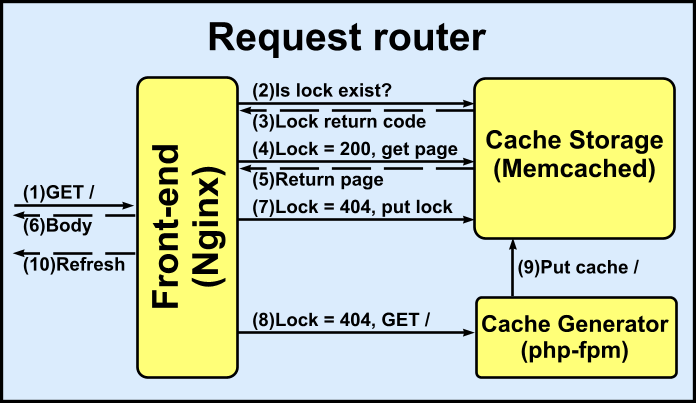
\includegraphics[width=8cm]{14_kraev.png}}
\label{pic:kraev}
%\caption{Приложения по категориям}
\end{figure}

По этой схеме Nginx выступает в качестве маршрутизатора между хранилищем кэша и кэш-генератором, вызывая для обработки запросов LUA-скрипт. Таким образом, страницы всегда отдаются из кэша. Если же кэша не существует, отправляется запрос для его генерации, а клиент перенаправляется на refresh-страницу, которая заставляет отправить запрос повторно через заданное время. Кэш имеет expire time = 0, что означает,  что он никогда не будет удален. Для обновления кэша используется lock с ограниченным expire time (в зависимости от запрашиваемой страницы), и когда expire time истекает "--- кэш регенерируется и помещается поверх старого. Также lock имеет еще одну важную функцию: его наличие предотвращает отправку запросов на генерацию из других фронтендов, если  автомасштабируемый кластер стал раздуваться, и в группе находится больше одного инстанса. 

Общее хранилище решает проблему прегенерации кэша. Так, при добавлении нового инстанса, он сразу вступает в распределение нагрузки, используя кэш из общего хранилища.  Такой подход позволяет ускорить ресурсы не только с Wordpress, а в принципе любой ресурс с ПО, написанным на любом коде, из которого генерируется HTML.

\section*{Save and profit!}

Использование данных технологий позволило нашей компании существенно снизить затраты на техническое обеспечение интернет-ресурса \url{theuptake.org}. Заменив 8 физических серверов (80--90\% времени они простаивали, но были необходимы из-за периодических резких всплесков посещений после публикации новостей), на 1 large-инстанс, на котором хранится общий контент и кэш, 1 RDS-инстанс, в котором лежит БД и автомасштабируемая группировка, работающая во время простоя с 1 smallинстанса и раздуваемая до кластера, размер которого определяет нагрузка. В дополнение к экономии (т.к. сегодня мы платим только за пики) мы многократно повысили скорость отдачи контента,  доступность и отказоустойчивость ресурса. 

\end{document}

\documentclass[10pt, a5paper]{article}
\usepackage{ucs}
\usepackage[utf8]{inputenc}
\usepackage[T2A]{fontenc}
\usepackage[english, russian]{babel}
\usepackage{hyperref}
\usepackage{geometry}
\frenchspacing

\begin{document}

\title{Способы повышения производительности высоконагруженных проектов на CMS Drupal}

\author{Виталий Иоскевич\footnote{Минск, Беларусь}}
\date{}
\maketitle
\renewcommand{\abstractname}{Abstract}
\begin{abstract}
Drupal is a popular CMS/CMF used to power the different types of web-projects worldwide. The desire of developers to make their system competitive in terms of functionality and flexibility sooner or later leads to increase of server load and reduced performance. Extensive functionality, flexibility in configuration and extensibility through third-party modules are undoubtedly a huge advantage, enabling to carry out projects of varying complexity and purpose, but the price often is a poor performance of high loaded Drupal-powered sites.
In our review we are going to revise existing standard methods of Drupal performance optimization (both server- and client-side) and demonstrate custom solutions that can be applied to some of the critical areas of Drupal-powered high-loaded web-site. In our real-life example we are going to show how to build Google Map page, capable to show thousands of markers based on Drupal content nodes.*

Насчет изменения предложения - "/Кэширование критично как для анонимов, так и для авторизованных пользователей. Используется Pressflow/Varnish/" - нет проблем. 
\end{abstract}
  
Drupal (7-ая, текущая версия) является достаточно развитой системой управления контентом. Стремление разработчиков сделать свою систему универсальной и более функциональной, чем у конкурентов, рано или поздно приводит к тому, что возрастают нагрузки на сервер, снижается быстродействие. Обширный функционал, гибкость в конфигурировании и расширяемость посредством сторонних модулей несомненно являются огромным преимуществом, благодаря которому позволяет выполнять проекты различной сложности и назначения, но плата за него --- низкая производительность готового решения. 

Чем больше число использованных на сайте сторонних модулей (в т.~ч. собственной разработки), тем ниже производительность сайта при больших нагрузках (большом количестве посетителей), а именно при построении сайтов с предполагаемым большим числом  посетителей никак не обойтись стандартным функционалом CMS. Таким образом, данная CMS оказывается весьма требовательной к ресурсам сервера, и в большинстве случаев проблема  решается выбором специализированных дорогих хостингов --- выделенный сервер или несколько серверов. 

Но и при ограниченных возможностях сервера есть способы улучшения производительности сайта. Стандартной системы кэширования Drupal достаточно для нормальной работы среднего сайта при неинтенсивной посещаемости, однако для случая высокой нагрузки на сайт этой системы недостаточно.

\section*{Основные методы повышения производительности Drupal:}
\begin{itemize}
	\item включить кэш в модулях, позволяющих кэширование (таких как Views, Panels, Feeds, SWF Tools и т.п.);
	\item увеличить время жизни кэша для стандартной системы кэширования Drupal. При этом надо иметь ввиду, что посетители будут видеть обновления содержимого значительно позже;
	\item если нет большой необходимости в статистике, можно выключить стандартные модули statistics и database logging. Они используют дополнительные запросы к БД при загрузке страницы. Кроме того, можно найти альтернативу данным модулям;
	\item использовать модуль CSS Gzip. Уменьшает размер файлов и количество http-запросов;
	\item использовать модуль Global Redirect. Предотвращает кэширование дубликатов содержимого сайта по ссылкам псевдонимам (синонимам) в случае использования <<Clean URL>>;
	\item использовать модуль Javascript Aggregator. Настройки Drupal позволяют объединить js-файлы, однако этот модуль позволяет еще и уменьшить конечный размер передаваемого файла;
	\item заменить системный cron на более функциональный модуль Elysia Cron. В отличие от системного, Elysia Cron позволяет распределить задачи по времени одна за одной, а не все вместе, при этом снижая пиковую нагрузку на сервер;
	\item перенести вызов javascript вниз станицы;
	\item помещать сторонние библиотеки вне каталога модулей /sites/all/modules --- например, в /sites/all/libraries. В таком случае Drupal не будет просматривать ненужные ему файлы;
	\item конвертировать таблицы MySQL в UTF8 InnoDB;
	\item создать индексы для медленных запросов Views. Желательно проанализировать такие запросы и увеличить производительность созданием индексов для полей;
	\item использовать ImageMagick вместо стандартной GD image library, т.~к. он лучше использует ресурсы сервера и дает лучшее качество изображений;
	\item использовать модуль Content Delivery Network integration. Он позволяет распределить файлы на множество отделенных друг от друга серверов. При этом снижается динамическая нагрузка на сервер, но требуется дополнительная плата за каждый сервер;
\end{itemize}

Наиболее продуктивным способом увеличения производительности является использование отдельной  эффективной системы кэширования.

{\bf Boost}. Одна из лучших систем кэширования для shared hosts. Cоздает копии html-станиц, которые генерирует Drupal, и хранит их в каталоге cache. Используя правила <<.htaccess>>, Boost проверяет, существует ли необходимый файл. Если да, то загружает статичный html, полностью избегая Drupal/PHP/MySQL. Если нет,  генерирует файл. Старые файлы удаляются по cron для того, чтобы выводимое содержимое сайта оставалось свежим (актуальным).

{\bf Memcache}. Серверная система кэширования, сохраняющая страницы сайта в оперативной памяти сервера. Все что необходимо для эффективной работы в данном случае --- быстрое ОЗУ большого объема. Его можно успешно использовать как для кэширования анонимных пользователей, так и для зарегистрированных. Но возможен и вариант, когда Memcache кэширует зарегистрированных пользователей, а Boost используется для кэширования анонимов. К преимуществам варианта можно отнести возможность кэширования анонимов и зарегистрированных пользователей, а к недостаткам --- то, что нужен хотя бы VPS, c достаточной оперативной памятью и невозможность работы на shared hosting.

{\bf APC(Alternate PHP Cache)}. Система кэширования op-code для серверов Apache. Подход весьма эффективен при большом числе активных модулей на сайте. Суть системы заключается в кэшировании компилированного байт-кода PHP-скрипта для того, чтобы избежать расходов ресурсов сервера на разбор и компиляцию исходного кода при каждом запросе. Для дальнейшего повышения производительности кэшированный код хранится в общей памяти и непосредственно выполняется оттуда, тем самым сводя к минимуму количество медленных операций чтения файлов и копирования в памяти во время выполнения.
К преимуществам относится ускорение компиляции скриптов Drupal и уменьшение использования ресурсов сервера, к недостаткам --- необходимость произвести специальное конфигурирование сервера.

{\bf Varnish(reverse proxy http-accelerator)}. Данная система выступает на первом плане над сервером Apache, PHP и Drupal. Varnish сохраняет кэшированное содержимое в оперативной памяти, и таким образом экономит ресурсы на загрузке Apache и Drupal. В результате этого Varnish предоставляет высокую производительность для кэшированных страниц для анонимных пользователей и является предпочтительным вариантом для сложных ресурсоемких сайтов, требующих значительной  масштабируемости. Для работы с Drupal 6 необходима была отдельная <<оптимизированная>> сборка дистрибутива под названием PressFlow и установка модуля интеграции Varnish HTTP Accelerator Integration. Для текущей версии Drupal достаточно установки модуля.

\section*{Пример проекта с высокой нагрузкой --- 350.org (Drupal 6)}

К характеристикам проекта можно отнести следующие: 
\begin{itemize}
	\item 150 000+  уникальных посетителей в день
	\item 6000+ ивентов, созданных пользователями
	\item ~500 авторизованных пользователей в среднем постоянно на сайте
	\item Самая посещаемая страница: карта ивентов (/map)
\end{itemize}

Кэширование критично как для анонимов, так и для авторизованных пользователей. Используется Pressflow/Varnish

Cпециальные меры и собственные разработки для повышения производительности включают:
\begin{itemize}
	\item Отказ от Views для генерации больших массивов данных
	\item  XML файл на диск вместо DB кэш (плюсы/минусы)
	\item Кэширование на диск всех RSS фидов
	\item Ajax запросы информации для маркеров на карте
\end{itemize}

\end{document}





\documentclass[10pt, a5paper]{article}
\usepackage{pdfpages}
\usepackage{parallel}
\usepackage[T2A]{fontenc}
\usepackage{ucs}
\usepackage[utf8x]{inputenc}
\usepackage[polish,english,russian]{babel}
\usepackage{hyperref}
\usepackage{rotating}
\usepackage[inner=2cm,top=1.8cm,outer=2cm,bottom=2.3cm,nohead]{geometry}
\usepackage{listings}
\usepackage{graphicx}
\usepackage{wrapfig}
\usepackage{longtable}
\usepackage{indentfirst}
\usepackage{array}
\newcolumntype{P}[1]{>{\raggedright\arraybackslash}p{#1}}
\frenchspacing
\usepackage{fixltx2e} %text sub- and superscripts
\usepackage{icomma} % коскі ў матэматычным рэжыме
\PreloadUnicodePage{4}

\newcommand{\longpage}{\enlargethispage{\baselineskip}}
\newcommand{\shortpage}{\enlargethispage{-\baselineskip}}

\def\switchlang#1{\expandafter\csname switchlang#1\endcsname}
\def\switchlangbe{
\let\saverefname=\refname%
\def\refname{Літаратура}%
\def\figurename{Іл.}%
}
\def\switchlangen{
\let\saverefname=\refname%
\def\refname{References}%
\def\figurename{Fig.}%
}
\def\switchlangru{
\let\saverefname=\refname%
\let\savefigurename=\figurename%
\def\refname{Литература}%
\def\figurename{Рис.}%
}

\hyphenation{admi-ni-stra-tive}
\hyphenation{ex-pe-ri-ence}
\hyphenation{fle-xi-bi-li-ty}
\hyphenation{Py-thon}
\hyphenation{ma-the-ma-ti-cal}
\hyphenation{re-ported}
\hyphenation{imp-le-menta-tions}
\hyphenation{pro-vides}
\hyphenation{en-gi-neering}
\hyphenation{com-pa-ti-bi-li-ty}
\hyphenation{im-pos-sible}
\hyphenation{desk-top}
\hyphenation{elec-tro-nic}
\hyphenation{com-pa-ny}
\hyphenation{de-ve-lop-ment}
\hyphenation{de-ve-loping}
\hyphenation{de-ve-lop}
\hyphenation{da-ta-ba-se}
\hyphenation{plat-forms}
\hyphenation{or-ga-ni-za-tion}
\hyphenation{pro-gramming}
\hyphenation{in-stru-ments}
\hyphenation{Li-nux}
\hyphenation{sour-ce}
\hyphenation{en-vi-ron-ment}
\hyphenation{Te-le-pathy}
\hyphenation{Li-nux-ov-ka}
\hyphenation{Open-BSD}
\hyphenation{Free-BSD}
\hyphenation{men-ti-on-ed}
\hyphenation{app-li-ca-tion}

\def\progref!#1!{\texttt{#1}}
\renewcommand{\arraystretch}{2} %Іначай формулы ў матрыцы зліпаюцца з лініямі
\usepackage{array}

\def\interview #1 (#2), #3, #4, #5\par{

\section[#1, #3, #4]{#1 -- #3, #4}
\def\qname{LVEE}
\def\aname{#1}
\def\q ##1\par{{\noindent \bf \qname: ##1 }\par}
\def\a{{\noindent \bf \aname: } \def\qname{L}\def\aname{#2}}
}

\def\interview* #1 (#2), #3, #4, #5\par{

\section*{#1\\{\small\rm #3, #4. #5}}

\def\qname{LVEE}
\def\aname{#1}
\def\q ##1\par{{\noindent \bf \qname: ##1 }\par}
\def\a{{\noindent \bf \aname: } \def\qname{L}\def\aname{#2}}
}

\begin{document}
\title{Открытые протоколы --- основа распределенных социальных сетей}
\author{Александр Загацкий\footnote{Витебск, Беларусь, \url{http://zag.ru}, \url{me@zag.ru}}}
\date{}
\maketitle

\begin{abstract}Distributed networks help users to control their online identity in the Internet.
Their key feature is absence of a central server. Nodes
in the network belong to each one of its
participants, and software runs on user's computer
or on trusted server. User determines the distribution policy
of his data.
Distributed social networks are built upon open technologies, such as Atom,
WebFinder, OpenID/OAuth, Salmon, ActivityStreams and etc.
Most of developed distributed networks are opensourced and under
development. Some of them are available to use, i.e. 
SatausNet --- the open source microblogging platform that
helps you share and connect in real-time within your own domain. Yet
another distibuted social network OneSocialWeb is a dream of the world where
all social networks are connected and work together similar
to email.
\end{abstract}
Весной этого года в одном из дата-центров провайдера облачного хостинга
Amazon EC2 произошел сбой \cite{zag1}, в результате чего перестали
 функционировать такие сервисы как Friendfeed, Quora, Reddit, Hootsuite,
 foursquare. По неожиданной случайности это совпало с началом судного дня
 в сериале "Терминатор: Битва за будущее". По сюжету фильма в этот день
 военная компьютерная сеть SkyNet, управляющая военными роботами вышла из
 под контроля человека и произвела ряд ядерных атак на человечество. К
 каким последствиям может привести утрата контроля над персональными
 данными, созданными пользователями в сети и раскрывающие отдельные
 моменты их личной жизни?

 Этот случай заставил задуматься о надежности социальных сервисов и
 сохранности пользовательских данных. Помимо этого за социальными
 сервисами стоят организации. Как следствие, функционирование сервиса
 зависит зачатую от материального положения владельца сервиса. Таким
 образом, сохранность личных данных и контроль над доступом к ним являются
 актуальной задачей для пользователей Интернет.

 Отчасти решить очерченную задачу призваны децентрализованные
 (распределенные) социальные сети. Характерной их особенностью, является
 отсутствие центрального сервера. Узлы сети принадлежат каждому из ее
 участников, а программное обеспечение функционирует на компьютере
 пользователя или на доверенном сервере. При этом пользователь
 самостоятельно определяет политику распространения его данных.

 В основе функционирования распределенных сетей лежат открытые протоколы.
 Ключевыми из них являются следующие:

 \subsubsection*{Atom/RSS}
% \begin{figure}[ht]
%\centering{
\includegraphics{16_zag1_atom-logo.png}}
%\end{figure}

    Формат синдикации Atom основан на XML и позволяет описывать наборы
    веб-ресурсов. Например: новостные ленты, анонсы статей в блоге,
    галереи фотографий и тому подобное. Формат описан в RFC 4287 \cite{zag2}.

    \subsubsection*{XRD}
 Стандарт описания ресурса доступен в \cite{zag3}. Представляет собой
    последовательное описание данных аккаунта в формате XML. Среди
    данных --- сведения о серверах аутентификации, публичные криптоключи и т.д.

    \subsubsection*{WebFinder}
% \begin{figure}[ht]
%\centering{
\includegraphics{16_zag1_WebFinger.png}}
%\end{figure}
    Протокол, позволяющий идентифицироваться пользователю. В качестве
    идентификации используется запись вида 
    
    \verb!acct:joe@example.com!

    По данному адресу устанавливается сервер с учетной записью
    пользователя и извлекаются XRD-записи.

 \subsubsection*{OpenID/OAuth}
%  \begin{figure}[ht]
%\centering{
\includegraphics{16_zag1_penid-icon.png}}
%\end{figure}
    Протоколы аутентификации и авторизации. Позволяют повысить
    безопасность при взаимодействии нескольких независимых сервисов.

    \subsubsection*{Pubsubhubbub}
%   \begin{figure}[ht]
%\centering{
\includegraphics{16_zag1_pubsubhubbub.png}}
%\end{figure}
    Протокол позволяет сообщать об обновлениях другим ресурсам. При этом
    используются так называемые хабы, которые сообщают об изменениях на
    основном ресурсе подписчикам. Такая схема позволяет реализовать 
    Push-канал обновлений, снизив нагрузку на источник изменений.

    Авторами являются сотрудники Google: Brad Fitzpatrick and Brett
    Slatkin. Источник обновления децентрализуется. Адрес hub для
    обновлений указывается в RSS/Atom в следующем формате:

\noindent     \verb!<link rel="hub" href="http://myhub.example.com/endpoint"/>!


     \subsubsection*{Salmon}
%    \begin{figure}[ht]
%\centering{
\includegraphics{16_zag1_customLogo.png}}
%\end{figure}
    Этот протокол позволяет отправлять действия по отношению к объекту
    (например, статье или заметке) с агрегаторов в оригинальный
    источник. Например, Salmon используется для сбора комментариев к
    оригинальной статье с других сайтов, на которых статья была
    опубликована.

    Адрес для отправки обновлений указан в RSS/Atom:

\noindent        \verb!<link rel="salmon"! \linebreak
\verb!href="http://example.org/salmon-endpoint"/>!

    Особенностью данного протокола является крипто-подпись сообщений,
    которая позволяет решить проблемы со спамом. Для получения
    публичного ключа используется формат XRD.

    \subsubsection*{ActivityStreams}
%    \begin{figure}[ht]
%\centering{
\includegraphics{16_zag1_icon-lg.png}}
%\end{figure}
    Формат описания активности пользователя на ресурсах. Благодаря этому
    формату происходит уведомление узлов распределенной сети о действиях
    пользователей: написании комментария, выставление оценки <<нравится>>,
    публикации фотографий и т.д. Из форматов доступны как JSON, так и
    расширения Atom \cite{zag4}.

    \subsubsection*{XMPP}
    Протокол обмена XMPP (<<Jabber>>) лежит в основе транспорта между
    узлами нескольких распределенных сетей. В качестве клиента
    используется как десктопные программы, так и мобильные версии.

    \subsubsection*{Portable Contacts}
    Протокол безопасного предоставления данных о своих контактах внешним
    сервисам \cite{zag5}. При этом используется протокол OAuth, и
    пользователь управляет доступом к своему списку контактов.

 Среди проектов создания распределенных социальных сетей \linebreak можно отметить
 следующие:
 \begin{description}
	 \item[StatusNet] \cite{zag6}\\
   Открытую платформу для микроблоггинга (аналог Twitter) StatusNet
    можно установить на собственном домене. Платформа предназначена для
    коллективного использования. Лицензия: AGPLv3.
    \item[GNU Social] \cite{zag7}\\
    Соответствует философии Unix: маленькие программы делают маленькие
    работы. По возможностям близка к Status.net: микроблоггинг. Лицензия:
    AGPLv3.
    \item[Diaspora] \cite{zag8}\\
    Проект Diaspora, созданный по инициативе четырех студентов,
    предназначен для персонального использования: ведения микроблога,
    публикации фотографий. Лицензия: AGPL-3.0.
    \item[friendika] \cite{zag9}\\
    Возможности: cервер профилей и поддержка ряда других сетей
    (Diaspora, Google Buzz, Identi.ca, Twitter), поддержка \linebreak шифрования
    между серверами. Лицензия: BSD License.
    \item[OneSocialWeb] \cite{zag10}
    Данная сеть микроблоггинга использует в качестве транспорта протокол
    XMPP \cite{zag11}. В качестве идентификатора пользователя
    используется jabber ID, часть протоколов адаптирована для
    использования в Jabber-сети. Лицензия: Apache 2.
\end{description}
 Это небольшая часть из разрабатываемых проектов, позволяющих
 пользователю сети управлять своими данными и быть независимым в контроле
 над персональной информацией. Тем не менее, очевидно, что персональные
 данные являются основной составляющей социальной жизни в сети и
 определять политику их использования может только пользователь.
\begin{thebibliography}{99}
	\bibitem{zag1} "Судный день для моих персональных данных". \url{http://zag.ru/a4BR2}
	\bibitem{zag2} RFC 4287: The Atom Syndication Format. \url{http://tools.ietf.org/html/rfc4287}
	\bibitem{zag3} Extensible Resource Descriptor (XRD). \url{http://docs.oasis-open.org/xri/xrd/v1.0/xrd-1.0.html}
	\bibitem{zag4} Формат оповещений Activity Streams. \url{http://activitystrea.ms/}
	\bibitem{zag5} Протокол Portable Contacts. \url{http://code.google.com/intl/ru-RU/apis/contacts/docs/poco/1.0/developers_guide.html}
	\bibitem{zag6} Платформа для микроблоггинга StatusNet. \url{http://status.net/}
	\bibitem{zag7} Распределенная сеть GNU Social. \url{http://foocorp.org/projects/social/}
	\bibitem{zag8} Социальная сеть Diaspora. \url{http://www.joindiaspora.com/}
	\bibitem{zag9} Распределенная сеть Friendika. \url{http://project.friendika.com}
	\bibitem{zag10} Социальная сеть OneSocialWeb, построенная на основе протокола XMPP. \url{http://onesocialweb.org/}
	\bibitem{zag11} XMPP - открытый протокол обмена сообщениями и информацией о статусе. \url{http://ru.wikipedia.org/wiki/XMPP}
\end{thebibliography}

\end{document}

\documentclass[10pt, a5paper]{article}
\usepackage{ucs}
\usepackage[utf8]{inputenc}
\usepackage[T2A]{fontenc}
\usepackage[english, russian]{babel}
\usepackage{hyperref}
\usepackage{geometry}
\usepackage{listings}
\frenchspacing
\begin{document}
\title{Perl 6 Pod --- формат ведения документации}
\author{Александр Загацкий\footnote{Витебск, Беларусь, \url{http://zag.ru}, \url{me@zag.ru}}}
\date{}
\maketitle

\begin{abstract}
Pod is an evolution of Perl 5's POD markup. Compared to POD, Perl 6's
Pod is much more
uniform, somewhat more compact, and considerably more
expressive. Established in 2005, specification
has undergone several revisions and is currently stable. The
specification is written in Perl 6 Pod and is a
good means of testing the implementations.
There are several implementations in Perl 5 and Perl 6.
Presentation covers the differences from Perl 5 POD, key features and 
experience of Perl 6 Pod personal usage.
\end{abstract}

Формат разметки Perl 6 Pod перестал быть черновиком. В финальной версии
спецификации Synopsis 26 \cite{zag1pod} добавился ряд особенностей.
Никогда не еще не было настолько тесной интеграции программного кода и
документации к нему.

Так, добавился специальный тип блоков документации --- блоки-деклараторы.
Данные блоки предваряются специальным комментарием \verb!#=!, за которым
следует текст документации. Оформленные блоки документации ассоциируются
с делараторами подпрограмм, а так же переменных. Уникальной особенностью
является тот факт, что эти блоки документации становятся доступными
через специальный атрибут \verb!.WHY!. Например:

\begin{lstlisting}[language={Perl}]
 sub fu (           #= This text stored in &fu.WHY
  Any     $bar,    #= This text stored in $bar.WHY
  Mode    :$baz   #= This text stored in $baz.WHY
    ) { ... }

 #= This is a special chainsaw
 my SwissArmy $chainsaw    #= (It has a rocket launcher)

 say $chainsaw.WHY; # prints: This is a special chainsaw
                   #         (It has a rocket launcher)
\end{lstlisting}


В приведенном примере текст документации к переменной \verb!$chainsaw!
становится доступным из программного кода. В указанном примере блок кода
будет выведен на экран:
\begin{lstlisting}[language={Perl}]
 say $chainsaw.WHY; # prints: This is a special chainsaw
                   #         (It has a rocket launcher)
\end{lstlisting}

Уникальна сама концепция, а именно доступ программного кода к
документации по нему. То есть становится возможным менять логику
программы в зависимости от описанной в документации!

Еще одним примером интеграции документации и кода являются
контекстуальные псевдонимы. Для их определения используется директива
\verb!=alias!. Например:
\begin{lstlisting}[language={Perl}]
 # This is actual code...
 sub hash_function ($key)
 *=alias HASHCODE*
 {
    my $hash = 0;
    for $key.split("") -> $char {
        $hash = $hash*33 + $char.ord;
    }
    return $hash;
 }
	   \end{lstlisting}

В данном примере определяется псевдоним HASHCODE. Его значением
является следующий за ним программный блок. Теперь, чтобы привести в
документации пример кода достаточно указать имя псевдонима внутри кода
форматирования \verb!A<>!:
\begin{lstlisting}[language={Perl}]
 =begin pod
 An ancient (but fast) hashing algorithm is used:
 =begin code :allow<A>
  A<HASHCODE>
 =end code
 =end pod
\end{lstlisting}

В результате в документации будет вставлен блок кода из программы:
\begin{lstlisting}[language={Perl}]
 An ancient (but fast) hashing algorithm is used:

    my $hash = 0;
    for $key.split("") -> $char {
        $hash *= 33;
        $hash += $char.ord;
    }
    return $hash;
	   \end{lstlisting}

Это позволяет избежать ручного копирования блоков кода и последующую
актуализацию документации.


\begin{thebibliography}{9}
	\bibitem{zag1pod} Спецификация формата Pod (Synopsis 26). \url{https://github.com/zag/specs/raw/master/S26-documentation.pod}
\end{thebibliography}

\end{document}

\documentclass[10pt, a5paper]{article}
\usepackage{ucs}
\usepackage[utf8]{inputenc}
\usepackage[T2A]{fontenc}
\usepackage[english, russian]{babel}
\usepackage{hyperref}
\usepackage{geometry}
\frenchspacing

\begin{document}

\title{LeechCraft: открытый модульный интернет-клиент}

\author{Рудой Г. И.\footnote{Московский физико-технический институт, \url{0xd34df00d@gmail.com}}, Линкин О. Е.\footnote{Министерство Обороны Республики Беларусь, MaledictusDeMagog@gmail.com}}
\date{}
\maketitle

\begin{abstract}
LeechCraft, the open source modular
cross-platform internet client written in C++/Qt, is reviewed mostly from the
technical perspective. Design decisions are described as far as solutions of
the problems faced during development and arising from the modular
nature of the application. Other aspects of open development are also
briefly considered, such as building a community or future goals. 
The paper should be of high interest to those developing highly modular
applications or general open source projects.
\end{abstract}

LeechCraft --- это открытый модульный кросс-платформенный
интернет-клиент. LeechCraft ориентирован на выполнение типичных
пользовательских задач, связанных с интернетом, в том числе:
\begin{itemize}
	\item просмотр веб-страниц;
	\item чтение лент новостей;
	\item скачивание файлов;
	\item обмен мгновенными сообщениями. 
\end{itemize}
В то же время реализованы и другие функции: например, менеджер
пакетов, работающий в пространстве пользователя, простой текстовый
редактор, медиа-плеер.

Модульность приложения означает, что все задачи в LeechCraft
выполняются загружаемыми модулями, которые при желании можно отключать
либо не устанавливать. Модули также могут взаимодействовать друг с
другом: например, модуль для чтения лент новостей использует модуль
поддержки протокола HTTP для скачивания этих лент. Ядро приложения при
этом обеспечивает лишь загрузку модулей, корректный порядок их
инициализации, обеспечивает их взаимное взаимодействие и предоставляет
некоторые базовые сервисы, например, сетевой кэш или базу данных
cookies.

Среди преимуществ такой архитектуры со слабо зависящими друг от друга
(а именно, от конкретной реализации) модулями можно отметить высокую
гибкость приложения, значительное снижение дублирования
функциональности и кодо-расширяемость, возможность заменять модули на
другие, выполняющие аналогичные функции, без изменения кода вне этих
модулей, и т.~д. Так, например, модуль поддержки скриптовых плагинов
позволяет произвольному модулю взаимодействовать со скриптами, даже
если этот модуль не имеет никакой прямой поддержки скриптинга.

Одним из выбранных способов реализации такой архитектуры является
взаимодействие модулей при помощи обмена сообщениями --- специальными
структурами данных с заданными правилами обработки. Один модуль
посылает сообщение по соответствующей шине приложения, а ряд других
модулей опрашивается на предмет возможности обработки этого сообщения,
и каждый из этих модулей может во время выполнения либо обработать
сообщение, либо отказаться от его обработки.

В то же время иногда необходимо тесное связывание модулей друг с
другом. Например, модуль блокировки рекламы в веб-браузере тесно
связан с самой реализацией браузера, и сделать его абстрагированным от
конкретного модуля браузера не представляется возможным, а система
поддержки стилей чатов в клиенте мгновенных сообщений связана с
реализацией самого IM-клиента. Для таких случаев обеспечивается
возможность прямого соединения модулей друг с другом (при этом один из
модулей считается плагином для другого модуля), а модули сами
определяют удобный им протокол взаимодействия.

Однако, помимо упомянутых преимуществ, поставленная задача
реализации конечной функциональности при помощи слабо зависящих друг
от друга модулей создает ряд проблем, часть из которых связана со
статичной природой выбранного языка реализации (C++) и отсутствием в
нем полноценной поддержки RTTI и какого-либо Reflection. Например, при
реализации вышеупомянутого модуля поддержки скриптовых плагинов
необходима возможность во время выполнения приложения определять
используемые другими модулями протоколы взаимодействия друг с другом,
так как прямое добавление информации о соответствующих протоколах на
этапе написания кода либо на этапе компиляции противоречит принципу
слабого связывания. Возможности интроспекции, предоставляемые
фреймворком Qt, позволяют успешно решить эту проблему при условии
соблюдения простых правил при написании модулей.

Другие вопросы, возникающие при разработке подобных приложений --- это
создание сообщества вокруг приложения и его общее позиционирование.
Социальный аспект открытой разработки является не менее важным, чем
технический, поэтому он также обсуждается в докладе.

\begin{thebibliography}{9}
	\bibitem{leechcraft1} LeechCraft Architecture --- \url{http://leechcraft.org/development-leechcraft-architecture}
	\bibitem{leechcraft2} Gamma et al. Design Patterns: Elements of Reusable Object-Oriented Software. Addison-Wesley, 1995
\end{thebibliography}


\end{document}





\documentclass[10pt, a5paper]{article}
\usepackage{pdfpages}
\usepackage{parallel}
\usepackage[T2A]{fontenc}
\usepackage{ucs}
\usepackage[utf8x]{inputenc}
\usepackage[polish,english,russian]{babel}
\usepackage{hyperref}
\usepackage{rotating}
\usepackage[inner=2cm,top=1.8cm,outer=2cm,bottom=2.3cm,nohead]{geometry}
\usepackage{listings}
\usepackage{graphicx}
\usepackage{wrapfig}
\usepackage{longtable}
\usepackage{indentfirst}
\usepackage{array}
\newcolumntype{P}[1]{>{\raggedright\arraybackslash}p{#1}}
\frenchspacing
\usepackage{fixltx2e} %text sub- and superscripts
\usepackage{icomma} % коскі ў матэматычным рэжыме
\PreloadUnicodePage{4}

\newcommand{\longpage}{\enlargethispage{\baselineskip}}
\newcommand{\shortpage}{\enlargethispage{-\baselineskip}}

\def\switchlang#1{\expandafter\csname switchlang#1\endcsname}
\def\switchlangbe{
\let\saverefname=\refname%
\def\refname{Літаратура}%
\def\figurename{Іл.}%
}
\def\switchlangen{
\let\saverefname=\refname%
\def\refname{References}%
\def\figurename{Fig.}%
}
\def\switchlangru{
\let\saverefname=\refname%
\let\savefigurename=\figurename%
\def\refname{Литература}%
\def\figurename{Рис.}%
}

\hyphenation{admi-ni-stra-tive}
\hyphenation{ex-pe-ri-ence}
\hyphenation{fle-xi-bi-li-ty}
\hyphenation{Py-thon}
\hyphenation{ma-the-ma-ti-cal}
\hyphenation{re-ported}
\hyphenation{imp-le-menta-tions}
\hyphenation{pro-vides}
\hyphenation{en-gi-neering}
\hyphenation{com-pa-ti-bi-li-ty}
\hyphenation{im-pos-sible}
\hyphenation{desk-top}
\hyphenation{elec-tro-nic}
\hyphenation{com-pa-ny}
\hyphenation{de-ve-lop-ment}
\hyphenation{de-ve-loping}
\hyphenation{de-ve-lop}
\hyphenation{da-ta-ba-se}
\hyphenation{plat-forms}
\hyphenation{or-ga-ni-za-tion}
\hyphenation{pro-gramming}
\hyphenation{in-stru-ments}
\hyphenation{Li-nux}
\hyphenation{sour-ce}
\hyphenation{en-vi-ron-ment}
\hyphenation{Te-le-pathy}
\hyphenation{Li-nux-ov-ka}
\hyphenation{Open-BSD}
\hyphenation{Free-BSD}
\hyphenation{men-ti-on-ed}
\hyphenation{app-li-ca-tion}

\def\progref!#1!{\texttt{#1}}
\renewcommand{\arraystretch}{2} %Іначай формулы ў матрыцы зліпаюцца з лініямі
\usepackage{array}

\def\interview #1 (#2), #3, #4, #5\par{

\section[#1, #3, #4]{#1 -- #3, #4}
\def\qname{LVEE}
\def\aname{#1}
\def\q ##1\par{{\noindent \bf \qname: ##1 }\par}
\def\a{{\noindent \bf \aname: } \def\qname{L}\def\aname{#2}}
}

\def\interview* #1 (#2), #3, #4, #5\par{

\section*{#1\\{\small\rm #3, #4. #5}}

\def\qname{LVEE}
\def\aname{#1}
\def\q ##1\par{{\noindent \bf \qname: ##1 }\par}
\def\a{{\noindent \bf \aname: } \def\qname{L}\def\aname{#2}}
}


\begin{document}
\title{Создание специализированного дистрибутива Linux для подключения к национальной GRID-сети}
\author{Денис Пынькин\footnote{Минск, Беларусь}}
\def\progref!#1!{\texttt{#1}}

\maketitle

\begin{abstract}
Unicore is ready"=to"=run system used as main platform for belarussian national GRID network. 
There are no Linux distributions for bare-metal Unicore installation and user"=friendly administration. 
Article describes steps to produce Linux server based on ALTLinux technologies with Unicore services working out of the box.
\end{abstract}

\section*{Сборка базового дистрибутива}
Современные дистрибутивы ALT Linux собираются с помощью инструмента mkimage,
который состоит из набора правил для утилиты make и вспомогательных скриптов 
и предоставляет базовый функционал для сборки образа Linux-системы. 
Фактически для создания своего собственного дистрибутива достаточно в 
правильном порядке и с правильными параметрами собрать из предоставляемых 
<<кирпичиков>> единое целое, что в общем-то является нетривиальной задачей.

Так было предпринято несколько попыток создать универсальные профили для mkimage,
но наиболее удачным и развитым оказался mkimage-profiles-desktop 
(в рассылках и на форумах часто сокращают до аббревиатуры M-P-D).

Далее, на примере создания дистрибутива Unicore для упрощения подключения к 
белорусской национальной научной GRID-сети, описывается как можно 
использовать M-P-D для создания собственного инсталляционного образа сервера.

Для начала необходимо получить правила сборки дистрибутива из git-репозитория:
\begin{verbatim}
git clone git://git.altlinux.org/people/boyarsh/packages/
 mkimage-profiles-desktop
\end{verbatim}

 Создать файл для пакетного менеджера apt с описанием репозитория и соответствующей 
 архитектурой, который необходимо расположить по пути {\tt \~/\$branch-\$arch.conf}, 
 в случае стабильного репозитория для Platform 6 и 64-битной архитектуры "--- \linebreak 
 {\tt \~/p6-x86\_64.conf}. В качестве минимума в этом файле должна содержаться 
 ссылка на файл с описаниями источников пакетов, для нашего примера "---
 {\tt \~/p6-sources-x86\_64.list}.

Например для белорусского зеркала ALT Linux эти файлы будут выглядеть следующим образом:

{\tt p6-x86\_64.conf}:
\begin{verbatim}
Dir::Etc::SourceList "/home/d4s/p6-sources-x86\_64.list";
\end{verbatim}

{\tt p6-sources-x86\_64.list}:
\begin{verbatim}
rpm [p6] ftp://ftp.mgts.by/pub/ALTLinux/p6/branch x86_64
 classic
rpm [p6] ftp://ftp.mgts.by/pub/ALTLinux/p6/branch noarch
 classic
\end{verbatim}

Для создания установочного диска своего сервера удобнее всего использовать 
профиль от Антона Фарыгина, который можно собрать в качестве теста, 
чтобы проверить работоспособность конфигурации. 
Например, таким образом можно собрать установочный диск для 64-битной 
архитектуры с дизайном Sisyphus:
\begin{verbatim}
archs=x86_64 ./make-distro server-light
 --with-branding=altlinux-sisyphus
\end{verbatim}

На консоль ничего не выводится, но это не страшно "--- <<все ходы записаны>>, 
а ход сборки протоколируется в файлы вида \linebreak <target>.<arch>.log или, в нашем 
случае, в файл \linebreak {\tt server-light.x86\_64.log}.

Получившийся образ диска сохраняется в домашнем каталоге {\tt ~/out/<target>} ({\tt ~/out/server-light/}).

Теперь можно приступать к созданию собственного сервера.

\section*{Модификация базового дистрибутива}
Модификация базового дистрибутива проводится с помощью дополнительных пакетов 
и изменения M-P-D для добавления своих правил сборки дистрибутива и 
списков программного обеспечения, которое будет доступно во время и после установки.

Все дополнительные пакеты условно можно разбить на две категории "--- функциональные и вспомогательные.

К функциональным относятся пакеты, которые содержат все необходимое для 
полноценного выполнения сервером той задачи, для которой он создается.
Для создания управляющего сервера Unicore, технически готового для включения 
в белорусский национальный GRID, это пакеты, содержащие сами сервисы Unicore: 
gateway, unicorex, xuudb и TSI. 
Кроме того, для полноценного управления вычислительным кластером необходим сервис 
управления пакетными задачами Torque, а по требованию операционного центра 
добавлено программное обеспечение учета ресурсов и система мониторинга Ganglia.

Кроме того разработаны специально для дистрибутива два дополнительных пакета:

\begin{itemize}
	\item unicore-grid-by --- содержит конфигурационные скрипты и \linebreak файлы, специфичные для белорусской GRID-сети.
	\item alterator-unicore-servers --- минимальный интерфейс для \linebreak настройки Unicore, реализованный в виде модуля к системе управления Alterator.
\end{itemize}

Вспомогательные пакеты необходимы только для корректной установки функционала, создания интерфейса либо на подготовительном этапе создания своего установочного диска.

Так можно выделить следующие пакеты:
\begin{itemize}
	\item installer-distro-unicore-server --- этот пакет содержит правила, 
		которые будут выполняться во время установки на различных этапах. 
		Например тут можно указать в каком порядке и какие шаги выполнять 
		программе-установщику, какие сервисы будут запускаться. Сюда же можно 
		добавлять скрипты для более тонкой настройки системы в процессе инсталляции.
	\item installer-feature-vm-unicore-server-stage2 --- этот пакет позволяет 
		подсказать программе-установщику какие разделы и какого размера должны 
		быть созданы жестком диске по умолчанию, а также точки монтирования 
		и предпочтительные файловые системы.
	\item branding --- пакет содержит все графические части, дизайн и, 
		несущественные для сервера, первоначальные пользовательские настройки 
		для оконных сред. Именно здесь можно поменять внешний вид веб"=интерфейса, 
		загрузчика, добавить свои картинки для слайд-шоу во время инсталляции.
\end{itemize}

\end{document}



\documentclass[10pt, a5paper]{article}
\usepackage{pdfpages}
\usepackage{parallel}
\usepackage[T2A]{fontenc}
\usepackage{ucs}
\usepackage[utf8x]{inputenc}
\usepackage[polish,english,russian]{babel}
\usepackage{hyperref}
\usepackage{rotating}
\usepackage[inner=2cm,top=1.8cm,outer=2cm,bottom=2.3cm,nohead]{geometry}
\usepackage{listings}
\usepackage{graphicx}
\usepackage{wrapfig}
\usepackage{longtable}
\usepackage{indentfirst}
\usepackage{array}
\newcolumntype{P}[1]{>{\raggedright\arraybackslash}p{#1}}
\frenchspacing
\usepackage{fixltx2e} %text sub- and superscripts
\usepackage{icomma} % коскі ў матэматычным рэжыме
\PreloadUnicodePage{4}

\newcommand{\longpage}{\enlargethispage{\baselineskip}}
\newcommand{\shortpage}{\enlargethispage{-\baselineskip}}

\def\switchlang#1{\expandafter\csname switchlang#1\endcsname}
\def\switchlangbe{
\let\saverefname=\refname%
\def\refname{Літаратура}%
\def\figurename{Іл.}%
}
\def\switchlangen{
\let\saverefname=\refname%
\def\refname{References}%
\def\figurename{Fig.}%
}
\def\switchlangru{
\let\saverefname=\refname%
\let\savefigurename=\figurename%
\def\refname{Литература}%
\def\figurename{Рис.}%
}

\hyphenation{admi-ni-stra-tive}
\hyphenation{ex-pe-ri-ence}
\hyphenation{fle-xi-bi-li-ty}
\hyphenation{Py-thon}
\hyphenation{ma-the-ma-ti-cal}
\hyphenation{re-ported}
\hyphenation{imp-le-menta-tions}
\hyphenation{pro-vides}
\hyphenation{en-gi-neering}
\hyphenation{com-pa-ti-bi-li-ty}
\hyphenation{im-pos-sible}
\hyphenation{desk-top}
\hyphenation{elec-tro-nic}
\hyphenation{com-pa-ny}
\hyphenation{de-ve-lop-ment}
\hyphenation{de-ve-loping}
\hyphenation{de-ve-lop}
\hyphenation{da-ta-ba-se}
\hyphenation{plat-forms}
\hyphenation{or-ga-ni-za-tion}
\hyphenation{pro-gramming}
\hyphenation{in-stru-ments}
\hyphenation{Li-nux}
\hyphenation{sour-ce}
\hyphenation{en-vi-ron-ment}
\hyphenation{Te-le-pathy}
\hyphenation{Li-nux-ov-ka}
\hyphenation{Open-BSD}
\hyphenation{Free-BSD}
\hyphenation{men-ti-on-ed}
\hyphenation{app-li-ca-tion}

\def\progref!#1!{\texttt{#1}}
\renewcommand{\arraystretch}{2} %Іначай формулы ў матрыцы зліпаюцца з лініямі
\usepackage{array}

\def\interview #1 (#2), #3, #4, #5\par{

\section[#1, #3, #4]{#1 -- #3, #4}
\def\qname{LVEE}
\def\aname{#1}
\def\q ##1\par{{\noindent \bf \qname: ##1 }\par}
\def\a{{\noindent \bf \aname: } \def\qname{L}\def\aname{#2}}
}

\def\interview* #1 (#2), #3, #4, #5\par{

\section*{#1\\{\small\rm #3, #4. #5}}

\def\qname{LVEE}
\def\aname{#1}
\def\q ##1\par{{\noindent \bf \qname: ##1 }\par}
\def\a{{\noindent \bf \aname: } \def\qname{L}\def\aname{#2}}
}

\begin{document}
\title{Методика оценки производительности нереляционных СУБД}
\author{Илья Бакулин\footnote{Москва, Россия}}
\date{}
\maketitle

\begin{abstract}
Non-relational databases are now widely used when building scalable web
applications. As NoSQL database systems each have its
own interface, so failing to choose the right product before beginning to
develop application will lead to complete rewrite of database work
layer. Most database testing frameworks can not be used to benchmark NoSQL 
DBMS. We have carried out testing with Yahoo Cloud Serving Berchmark to benchmark 
non-SQL systems.
\end{abstract}

В последнее время нереляционные базы данных часто используются при
построении веб-приложений, проектируемых с упором на масштабируемость.
Это становится своего рода <<модой>>. Но ведущие специалисты-архитекторы,
реализующие свои идеи во всемирно известных проектах (Facebook, Twitter,
Digg, Riak) сходятся во мнении, что нереляционные базы не могут
полностью заменить традиционные системы хранения данных. Большое
значение имеет выбор методики обоснования необходимости использования
нереляционной базы данных при разработке той или иной части функционала
приложения.

Ни одна NOSQL СУБД не поддерживает ставший стандартным в мире
реляционных БД язык запросов SQL. Одной из важнейших особенностей SQL
является то, что он позволяет разработчику абстрагироваться от
внутренней схемы хранения данных в конкретной СУБД. Хотя между
диалектами SQL, используемыми в различных реляционных СУБД, имеются
определённые различия, в целом для приложения логика работы с БД не
меняется при смене СУБД. Напротив, каждая NOSQL-СУБД предоставляет свой
интерфейс (API) для взаимодействия, свою схему хранения данных, и в
разных решениях они порой очень сильно отличаются. Попытка сменить
движок базы данных в процессе разработки может обернуться
непредвиденными сложностями, потерей времени, затраченного на
проектирование, программирование и тестирование нового решения, и в
конечном итоге ущербом для бизнеса компании.

Очевидно, необходимо тщательное тестирование возможных решений,
основанных на различных NOSQL-СУБД, перед собственно созданием системы.
Тестирование должно давать как можно более полное представление о том,
как ведёт себя выбранная СУБД в различных сценариях, типичных для
проектируемого веб-приложения.

Одной из систем оценки производительности, умеющих работать с
нереляционными базами данных, является написанный в Yahoo программный
пакет YCSB (Yahoo Could Serving Benchmark). Поддержка доступа к любой
базе данных может быть реализована путём написания адаптера,
обеспечивающего элементарные операции CREATE/REPLACE/UPDATE/DELETE.
Немаловажным является то, что становится возможным тестирование и
реляционных, и нереляционных БД с помощью одних и тех же тестовых сценариев.

Мы использовали пакет YCSB был использован для оценки
производительности хранилища данных для SMS-сообщений при выборе между
Cassandra и sharded MySQL. Для тестирования сначала была проведена
оценка распределения количества запросов на чтение, запись и обновление,
после чего написан конфигурационный файл для YCSB. После этого на одной
и той же машине были поочерёдно запущены кластеры Cassandra и MySQL и
проведено тестирование.

Результаты свидетельствуют о том, что при использовании
\linebreak Cassandra-кластера достигаются более высокие скорости записи в базу, но
более низкие скорости чтения, чем на MySQL. Это, в целом, подтверждается
и опытом других пользователей. В настоящее время рассматривается
возможность тестирования MongoDB, для которой в составе YCSB также
имеется адаптер.

\end{document}



\documentclass[10pt, a5paper]{article}
\usepackage{ucs}
\usepackage[utf8]{inputenc}
\usepackage[T2A]{fontenc}
\usepackage[english, russian]{babel}
\usepackage{hyperref}
\usepackage{geometry}
\frenchspacing
\begin{document}
\title{Свободные лицензии и российское законодательство: перспективы развития}
\author{Сергей Середа\footnote{Москва, Россия, Движение <<ПОтребитель>>, \url{serge_sereda@hotmail.com}}}
\date{}
\maketitle

\begin{abstract}
There is a number of legal issues with FOSS licensing in Russia which in some circumstances could be very serious. Moreover, prepared bill with changes to Civil Code contains initiatives which could only worsen this situation. FOSS enthusiasts in these circumstances should actively participate in debates on developement of the Russian Civil Code to prevent potential and fix actual compatibility problems of FOSS licences.
\end{abstract}

 До относительно недавнего времени в России <<свободное>> программное обеспечение существовало просто как явление, <<независимо>> от гражданского законодательства. Но по мере его распространения росло количество конечных пользователей, значительное число разработчиков стали участниками или даже основателями проектов разработки свободных программ, на внутреннем рынке появились сначала модемы и маршрутизаторы, работающие на GNU/Linux, затем стали продаваться телевизоры, видеопроигрыватели и приставки с этой же ОС <<на борту>>, приобрели популярность <<умные>> телефоны и планшетные ПК на базе ОС Android, развился бизнес по разработке программно-аппаратных решений на базе FOSS и оказанию услуг по их поддержке. Что же касается собственно операционной системы GNU/Linux, то на уровне Правительства она была названа целевой для сферы образования и госсектора в целом. 

На этом этапе правовая оценка свободного ПО стала необходимостью. Эта работа была проведена независимо разными исследователями, однако её результаты в целом схожи. В результате анализа текстов свободных лицензий и оценки используемого ими механизма лицензирования в контексте отечественного правового поля можно выделить следующие проблемные моменты:
\begin{enumerate}
	\item английский язык, на котором написано большинство свободных лицензий, начиная с GNU GPL;
	\item отсутствие явного указания территории, на которой действует лицензия;
	\item отсутствие явного указания срока действия лицензии;
	\item отсутствие явного указания суммы авторского вознаграждения (или безвозмездности лицензионного договора);
	\item несоблюдение письменной формы сделки при заключении лицензионного договора на свободное ПО;
	\item противоречие <<вирусного механизма>> лицензий на свободное ПО положениям п. 2 ст. 428 ГК РФ, п. 4 ст. 1233 ГК РФ и п. 4 ст. 1260 ГК РФ.
	\item эквивалентность безвозмездной лицензии на свободное ПО дарению, запрещённому для юридических лиц;
	\item отнесение экономии от бесплатного использования свободного ПО к внереализационным доходам, которые должны облагаться налогом, исчисляемым на основании рыночной стоимости использования аналогичного коммерческого ПО.
\end{enumerate}

Мнения специалистов о перечисленных коллизиях с отечественным законодательством разошлись: одна часть исследователей считает, что, несмотря на проблемные моменты, свободное ПО в России вполне законно (к ним, по большей части, относятся энтузиасты FOSS), другая же их часть считает, что противоречия с российским законодательством слишком серьёзны, чтобы считать свободные лицензии соответствующими Российским законам (этой точки зрения придерживаются <<ортодоксальные>> юристы). 

Следует также отметить, что это расхождение мнений касается лишь программ для ЭВМ и баз данных (для которых допустимы <<обёрточные>> лицензии). В отношении же свободных лицензий на другие объекты авторского права, в первую очередь --- литературные и музыкальные произведения, разногласий практически нет --- если подобные лицензионные договоры не заключаются в письменной форме, они (за небольшими исключениями) являются ничтожными на территории РФ.

Теоретически, указанная ситуация может быть разрешена совместными действиями общественных организаций, осуществляющих поддержку экосистемы свободных лицензий, и отечественного законодателя. Что касается общественных организаций, то, например, Creative Commons занимается адаптацией своих лицензий под законодательство РФ, в то время как Free Software Foundation лишь допускает такую возможность. Отечественный же законодатель, как выяснилось, придерживается в этом контексте довольно радикальной точки зрения. Авторы подготовленного пакета поправок в Гражданский Кодекс РФ считают, что несовместимость свободных лицензий и российского законодательств является системной, и проблему можно решить лишь созданием альтернативного механизма, дающего те же результаты, что и свободные лицензии.

Для этого предлагается ввести новый способ распоряжения исключительным правом --- временное предоставление произведения в пользование неограниченному кругу лиц на условиях, определённых правообладателем. Указанный механизм планируется зафиксировать в новой, шестой части статьи 1233 ГК РФ. Однако, чтобы им воспользоваться, правообладателю придётся разместить на официальном сайте федерального органа исполнительной власти по интеллектуальной собственности (\url{www.fips.ru}) заявление <<о предоставлении любым лицам возможности безвозмездно использовать принадлежащий ему результат интеллектуальной деятельности>> с указанием условий, на которых предоставляется эта возможность, а также срока действия заявления. При этом предоставлять произведение для использования публике можно только безвозмездно и только если на его использование не заключено ни одного возмездного лицензионного договора. Отказаться от подобного заявления или изменить зафиксированные в нём условия до истечения указанного в нём срока нельзя. 

Что касается собственно свободных лицензий, то авторы законопроекта предлагают трактовать их не как лицензионные договоры, а как описанные выше заявления. 

Однако, несмотря на озвученную выше позицию авторов поправок, этот же законопроект предполагает и расширение  положений об <<обёрточных>> лицензиях, к которым весьма близки лицензии на свободное ПО. Согласно предлагаемой формулировке новой части 5 статьи 1286 ГК РФ, заменяющей по смыслу часть 3, <<обёрточная>> лицензия \footnote{сам этот жаргонный термин в законе, естественно, не используется} --- это лицензионный договор, заключаемый <<в упрощенном порядке>> (в форме договора присоединения), но являющийся безвозмездным, <<если договором не предусмотрено иное>>. Следует отметить, что, намеренно или нет, но авторы поправок указанной формулировкой устраняют проблему отсутствия явного указания суммы авторского вознаграждения в текстах свободных лицензий. Правда, упрощённый порядок заключения лицензионного договора, к сожалению, так и остался привилегией программ для ЭВМ и баз данных, несмотря на активную торговлю <<электронными>> экземплярами  аудиовизуальных и литературных произведений в российской рознице.

Предлагаемые же поправки в текст статьи 1211 ГК РФ скажутся на свободных лицензиях однозначно негативно. Указанная статья определяет, право какой из сторон внешнеэкономической сделки применяется, если в соответствующем договоре об этом ничего не указано. Заключение лицензионного договора (в т.ч. свободной лицензии) с иностранным физическим или юридическим лицом, соответственно, регулируется указанной статьёй ГК. В соответствии с нынешней формулировкой этой статьи к лицензионным договорам, фиксирующим внешнеэкономическую сделку, по умолчанию применяется право страны лицензиара. В контексте существующих коллизий между свободными лицензиями и российским законодательством такая формулировка позволяет считать большую их часть несущественной в случаях, когда в России используется или дорабатывается свободное ПО, изначально созданное за рубежом.

В предлагаемой же новой редакции статьи 1211 ГК РФ, наоборот, говорится, что к лицензионным договорам должно применяться <<право страны, на территории которой лицензиату разрешается использование результата интеллектуальной деятельности>>. Это положение, правда, содержит оговорку о том, что <<если такое использование разрешается на территории одновременно нескольких стран>> то применяется <<право страны, где находится место жительства или основное место деятельности лицензиара>>, но она, к сожалению, проблемы не решает. Согласно части 3 статьи 1235 ГК РФ, в отсутствие явного указания на территорию, на которой согласно лицензионному договору предоставляется исключительное право, ею считается территория России, а поскольку в свободных лицензиях о территории ничего явно не говорится, то согласно будущей редакции статьи 1211 ГК РФ, к лицензиям на иностранное свободное ПО должно применяться право РФ.

Таким образом, общий эффект от планируемых изменений гражданского законодательства РФ на правовое положение свободных лицензий следует признать отрицательным. В отличие от Европейского союза, не просто признавшего свободные лицензии, но и разработавшего совместимую с ними собственную EUPL, в России лишь создаются дополнительные препятствия для этой <<инициативы снизу>> по саморегулированию рынка программного обеспечения. Такой подход, при его последовательном применении, приведёт к невозможности использования преимуществ свободного лицензирования российскими разработчиками и конечными пользователями, остановит обмен технологиями в области обработки данных и усилит зависимость России от поставщиков коммерческого программного обеспечения. Также, он прямо противоречит существующим и активно спонсируемым инициативам по внедрению свободного ПО в российском госсекторе, и создаёт существенные препятствия для развития российского инновационного бизнеса в сфере информационных технологий.

По мнению автора, свободное сообщество должно уделить особое внимание анализу планируемых изменений в российском гражданском законодательстве и их последствий для развития свободного ПО, а также принять активное участие в публичном обсуждении законопроекта и внесении в него корректив, которые бы позволили сократить число коллизий свободных лицензий с ГК РФ, вместо того, чтобы их усугублять.

\begin{thebibliography}{9}

	\bibitem{s1} Белопольский Э. Язык ничтожной сделки // Бизнес-адвокат, 1997, № 22. – Режим доступа к электрон. дан.: \url{http://www.juristlib.ru/book_305.html}.
	\bibitem{s2} Брауде–Золотарев М., Гребнев Г., Протасов П., Ралько А., Сербина Е. Лицензионные договоры и Российское законодательство. – Режим доступа к электрон. дан.: \url{http://vvv.srcc.msu.su/%7Eserbina/INFO-FOSS.RU/Digest3.pdf}
	\bibitem{s3} Проект ФЗ <<О внесении изменений в части первую, вторую, третью и четвертую Гражданского кодекса Российской Федерации, а также в отдельные законодательные акты Российской Федерации>>. – Режим доступа к электрон. дан.: \url{http://www.economy.gov.ru/minec/activity/sections/corpmanagment/civil_code/full_text_civil_code/140411_gk?presentationtemplate=docHTMLTemplate1&presentationtemplateid=2dd7bc8044687de796f0f7af753c8a7e&WCM_Page.ResetAll=TRUE&CACHE=NONE&CONTENTCACHE=NONE&CONNECTORCACHE=NONE}
	\bibitem{s4} Середа С.А. Открытое программное обеспечение: проблемы лицензирования и доказательства легальности. – Режим доступа к электрон. дан.: \url{http://consumer.nm.ru/osp_law.htm}
	\bibitem{s5} Середа С.А. Свободны ли в России <<свободные лицензии?>> // "Патенты и лицензии". – 2009. N4. – Режим доступа к электрон. дан.: \url{http://consumer.stormway.ru/foss&law.htm}
	\bibitem{s6} Тяпкина Е. Правовой статус GPL в России // <<Компьютерра>>. – 2002. №13 от 9 апреля. – Режим доступа к электрон. дан.: \url{http://offline.computerra.ru/print/offline/2002/438/17257/}.
\end{thebibliography}


\end{document}



\documentclass[10pt, a5paper]{article}
\usepackage{pdfpages}
\usepackage{parallel}
\usepackage[T2A]{fontenc}
\usepackage{ucs}
\usepackage[utf8x]{inputenc}
\usepackage[polish,english,russian]{babel}
\usepackage{hyperref}
\usepackage{rotating}
\usepackage[inner=2cm,top=1.8cm,outer=2cm,bottom=2.3cm,nohead]{geometry}
\usepackage{listings}
\usepackage{graphicx}
\usepackage{wrapfig}
\usepackage{longtable}
\usepackage{indentfirst}
\usepackage{array}
\newcolumntype{P}[1]{>{\raggedright\arraybackslash}p{#1}}
\frenchspacing
\usepackage{fixltx2e} %text sub- and superscripts
\usepackage{icomma} % коскі ў матэматычным рэжыме
\PreloadUnicodePage{4}

\newcommand{\longpage}{\enlargethispage{\baselineskip}}
\newcommand{\shortpage}{\enlargethispage{-\baselineskip}}

\def\switchlang#1{\expandafter\csname switchlang#1\endcsname}
\def\switchlangbe{
\let\saverefname=\refname%
\def\refname{Літаратура}%
\def\figurename{Іл.}%
}
\def\switchlangen{
\let\saverefname=\refname%
\def\refname{References}%
\def\figurename{Fig.}%
}
\def\switchlangru{
\let\saverefname=\refname%
\let\savefigurename=\figurename%
\def\refname{Литература}%
\def\figurename{Рис.}%
}

\hyphenation{admi-ni-stra-tive}
\hyphenation{ex-pe-ri-ence}
\hyphenation{fle-xi-bi-li-ty}
\hyphenation{Py-thon}
\hyphenation{ma-the-ma-ti-cal}
\hyphenation{re-ported}
\hyphenation{imp-le-menta-tions}
\hyphenation{pro-vides}
\hyphenation{en-gi-neering}
\hyphenation{com-pa-ti-bi-li-ty}
\hyphenation{im-pos-sible}
\hyphenation{desk-top}
\hyphenation{elec-tro-nic}
\hyphenation{com-pa-ny}
\hyphenation{de-ve-lop-ment}
\hyphenation{de-ve-loping}
\hyphenation{de-ve-lop}
\hyphenation{da-ta-ba-se}
\hyphenation{plat-forms}
\hyphenation{or-ga-ni-za-tion}
\hyphenation{pro-gramming}
\hyphenation{in-stru-ments}
\hyphenation{Li-nux}
\hyphenation{sour-ce}
\hyphenation{en-vi-ron-ment}
\hyphenation{Te-le-pathy}
\hyphenation{Li-nux-ov-ka}
\hyphenation{Open-BSD}
\hyphenation{Free-BSD}
\hyphenation{men-ti-on-ed}
\hyphenation{app-li-ca-tion}

\def\progref!#1!{\texttt{#1}}
\renewcommand{\arraystretch}{2} %Іначай формулы ў матрыцы зліпаюцца з лініямі
\usepackage{array}

\def\interview #1 (#2), #3, #4, #5\par{

\section[#1, #3, #4]{#1 -- #3, #4}
\def\qname{LVEE}
\def\aname{#1}
\def\q ##1\par{{\noindent \bf \qname: ##1 }\par}
\def\a{{\noindent \bf \aname: } \def\qname{L}\def\aname{#2}}
}

\def\interview* #1 (#2), #3, #4, #5\par{

\section*{#1\\{\small\rm #3, #4. #5}}

\def\qname{LVEE}
\def\aname{#1}
\def\q ##1\par{{\noindent \bf \qname: ##1 }\par}
\def\a{{\noindent \bf \aname: } \def\qname{L}\def\aname{#2}}
}

\begin{document}
\title{Виртуализация: история развития и технологии аппаратной поддержки}
\author{Павел Круглей\footnote{Минск, Беларусь, \url{nanoflat@gmail.com}}}
\date{}
\maketitle

\begin{abstract}
The history of virtualization and virtual machines is briefly discussed. The main types of virtualization are described, with focus on hardware-aided types: the first generation --- VT-x, VT-d, AMD-v technologies, the second one --- EPT / RVI, and the wave of technology, virtualization on mobile devices.\end{abstract}

\section*{Истоки (1970е)}
Всё начиналось с виртуализации памяти на машинах второго поколения в качестве средства расширения размеров оперативной памяти. Потребность в механизме расширения возникла из-за того, что использовавшаяся в то время память на ферритовых сердечниках стоила чрезвычайно дорого. Поэтому казалось логичным виртуализовать ее, то есть расширить за счет использования внешних устройств.

Впервые виртуальная машина появилась в 1961 году в супервизоре суперкомпьютера Atlas, который был разработан английской компанией Ferranti. В середине 60-х годов она была реализована в проект IBM M44/44X Project и машине IBM 7044. 

Следующим шагом в развитии идеи виртуализации стала концепция «виртуальной машины». Она появилась в 1965 году, когда исследователи в корпорации IBM предприняли экспериментальную попытку разделить компьютер на отдельные небольшие части. Это направление исследований привело к созданию многопользовательской операционной среды на машинах IBM System 370 и System 390 и операционной системы VM/ESA, совместно называемых генеалогической линией IBM VM (Virtual Machine). 

\section*{Виртуализация в СССР}

Проект СВМ/Система Виртуальных Машин являлся частью \linebreak комплексной программы ЕС ЭВМ (аналога IBM System/370), которая была начата в 1969 году. Адаптация системы IBM VM/370 Release 5 и программных продуктов ее окружения были основными целями в начале проекта СВМ.

СВМ (VM, и её ранняя версия CP/CMS) --- первая система, в которой была реализована технология виртуальных машин. Виртуализация в СВМ была последовательной и полной, в частности, на виртуальной машине можно было запустить другую копию системы СВМ, и так далее.

Архитектурно СВМ состояла из нескольких независимых компонентов. Центральным компонентом был монитор виртуальных машин (МВМ, IBM-овское название --- CP, Control Program), который управлял аппаратурой реальной ЭВМ и реализовывал набор виртуальных машин с заданной конфигурацией. Остальные компоненты представляли собой операционные системы или системонезависимые программы виртуальных машин, работавшие под управлением МВМ: подсистема диалоговой обработки (ПДО), подсистема сетевой передачи файлов (ПСП), подсистема логической коммутации абонентских пунктов (ПЛК), подсистема анализа дампов (ПАД), подсистема дистанционной передачи файлов (ПДП), подсистема контроля технических средств (ПКТ), средства генерации и обслуживания (СГО).

\section*{Типы виртуализации}
Обычно среди решений на основе виртуализации выделяют:
\begin{itemize}
	\item Эмуляция аппаратуры --- в хост-системе создается виртуальная машина, которая моделирует какую-то другую аппаратную архитектуру.
	\item Полная виртуализация --- использует виртуальную машину (гипервизор), которая выступает как посредник между гостевой операционной системой и реальным оборудованием. Некоторые инструкции защищенного режима должны перехватываться и обрабатываться внутри гипервизора, поскольку аппаратура не доступна непосредственно из операционных систем, доступ к ней предоставляется через гипервизор.
	\item Паравиртуализация --- требует модификации гостевой операционной системы, что является недостатком. Однако в этом случае обеспечивается производительность, близкая к производительности невиртуализированной системы. 
	\item Виртуализация уровня операционной системы --- операционная система одна и просто изолируются один от другого сервера, работающие под ее управлением.
\end{itemize}

\section*{Виртуализация в x86}
Впервые апаратная виртуализация была реализована в 386-х процессорах и носила название V86 mode. Этот режим позволял запускать параллельно несколько DOS"=приложений.

В 2005-м году компании Intel и AMD представили решения аппаратной  поддержки виртуализации --- INTEL VT и AMD-V. Были введены дополнительные инструкции для предоставления прямого доступа к ресурсам процессора из гостевых систем. Этот набор дополнительных инструкций носит название Virtual Machine Extensions (VMX). VMX предоставляет инструкции: VMPTRLD, VMPTRST, VMCLEAR, VMREAD, VMREAD, VMWRITE, \linebreak VMCALL, VMLAUNCH, VMRESUME, VMXON и VMXOFF.

Архитектура AMDV похожа на VT и предоставляет те же функциональные возможности, однако предусматривает также ряд дополнительных функций, отсутствующих у Intel VT.

Технология VT"=d позволяет избежать полной виртуализации \linebreak устройств ввода"=вывода. Используя VT"=d, VMM сможет «прикреплять» драйверы физических устройств к ВМ, что позволит гостевой ОС взаимодействовать с прикрепленным устройством без передачи управления VMM посредством механизма DMA (прямого доступа устройств к памяти минуя процессор).

%Второе поколение известно как NPT / EPT / HAP / RVI.
Следующее поколение аппаратной виртуализации предусматривает виртуализацию памяти. Это технологии AMD NPT (Nested Page Tables) / Intel EPT (Extended Page Tables). В целом технологии HAP (Hardware Assisted Paging), NPT, EPT и RVI (Rapid Virtualization Indexing) --- скорее изобретение маркетологов, так как на самом деле обозначают одно и то же. При  вызове операций из гостевой ОС, она отдает команду VMLAUNCH и начинает исполнять свой код, пользуясь далее инструкцией VMRESUME. Однако при операциях с памятью, гостевая ОС должна работать через монитор виртуальных машин VMM для управления памятью (механизм называется Shadow Paging). С использованием же Extended Page Tables (EPT) --- гостевая ОС может сама управляться со страницами памяти, включая контроль Page Faults, которые, кстати, проходят через гипервизор и вызывают VMEXIT. Инструкция VMEXIT --- это по сути передача управления Монитору виртуальных машин гипервизора, от которого ожидаются какие-то действия. Соответственно, чем меньше вызовов VMEXIT --- тем лучше.

\section*{Мобильная виртуализация}

Компания VMware продемонстрировала MVP (Mobile \linebreak Virtualization Platform), гипервизор для мобильных устройств, позволяющий одновременно использовать на телефоне такие платформы, как Google Android и Windows Mobile. Разработку планируется использовать для создания на мобильном устройстве дополнительного защищенного окружения для работы с приватными данными. 

Гипервизор MVP был продемонстрирован на планшетном ПК Nokia N800. 128MB ОЗУ и 256MB Flash оказалось достаточно для одновременного запуска двух виртуальных машин с Windows CE 6.0 и Google Android.

TRANGO --- гипервизор, а точнее виртуальный процессор, весящий 20 Kb, позволяющий запускать на мобильном устройстве с RISC-процессором от ARM или MIPS несколько гостевых ОС: eCos, Linux, Windows CE и другие ОС.

Компания Citrix объединила свои усилия с группой разработчиков Open Kernel Lab (OK Lab), создав уникальную мобильную платформу под рабочим названием Nirvana Phone.

Проект Nirvana Phone можно рассматривать как гибрид карманного смартфона и традиционных настольных гипервизоров. Виртуальный рабочий стол XenDesktop внутри коммуникаторa Nirvana Phone легко разворачивается в полноценное рабочее место с большим монитором, мышью и клавиатурой за счет применения мобильного клиентского модуля виртуализации OKL4 Microvisor 4.0. Сами разработчики считают, что оптимальным способом подключения периферийных устройств будет беспроводной интерфейс \linebreak Bluetooth "--- использование этого канала позволяет применять массу уже выпускаемых серийно устройств.
\end{document}



\documentclass[10pt, a5paper]{article}
\usepackage{pdfpages}
\usepackage{parallel}
\usepackage[T2A]{fontenc}
\usepackage{ucs}
\usepackage[utf8x]{inputenc}
\usepackage[polish,english,russian]{babel}
\usepackage{hyperref}
\usepackage{rotating}
\usepackage[inner=2cm,top=1.8cm,outer=2cm,bottom=2.3cm,nohead]{geometry}
\usepackage{listings}
\usepackage{graphicx}
\usepackage{wrapfig}
\usepackage{longtable}
\usepackage{indentfirst}
\usepackage{array}
\newcolumntype{P}[1]{>{\raggedright\arraybackslash}p{#1}}
\frenchspacing
\usepackage{fixltx2e} %text sub- and superscripts
\usepackage{icomma} % коскі ў матэматычным рэжыме
\PreloadUnicodePage{4}

\newcommand{\longpage}{\enlargethispage{\baselineskip}}
\newcommand{\shortpage}{\enlargethispage{-\baselineskip}}

\def\switchlang#1{\expandafter\csname switchlang#1\endcsname}
\def\switchlangbe{
\let\saverefname=\refname%
\def\refname{Літаратура}%
\def\figurename{Іл.}%
}
\def\switchlangen{
\let\saverefname=\refname%
\def\refname{References}%
\def\figurename{Fig.}%
}
\def\switchlangru{
\let\saverefname=\refname%
\let\savefigurename=\figurename%
\def\refname{Литература}%
\def\figurename{Рис.}%
}

\hyphenation{admi-ni-stra-tive}
\hyphenation{ex-pe-ri-ence}
\hyphenation{fle-xi-bi-li-ty}
\hyphenation{Py-thon}
\hyphenation{ma-the-ma-ti-cal}
\hyphenation{re-ported}
\hyphenation{imp-le-menta-tions}
\hyphenation{pro-vides}
\hyphenation{en-gi-neering}
\hyphenation{com-pa-ti-bi-li-ty}
\hyphenation{im-pos-sible}
\hyphenation{desk-top}
\hyphenation{elec-tro-nic}
\hyphenation{com-pa-ny}
\hyphenation{de-ve-lop-ment}
\hyphenation{de-ve-loping}
\hyphenation{de-ve-lop}
\hyphenation{da-ta-ba-se}
\hyphenation{plat-forms}
\hyphenation{or-ga-ni-za-tion}
\hyphenation{pro-gramming}
\hyphenation{in-stru-ments}
\hyphenation{Li-nux}
\hyphenation{sour-ce}
\hyphenation{en-vi-ron-ment}
\hyphenation{Te-le-pathy}
\hyphenation{Li-nux-ov-ka}
\hyphenation{Open-BSD}
\hyphenation{Free-BSD}
\hyphenation{men-ti-on-ed}
\hyphenation{app-li-ca-tion}

\def\progref!#1!{\texttt{#1}}
\renewcommand{\arraystretch}{2} %Іначай формулы ў матрыцы зліпаюцца з лініямі
\usepackage{array}

\def\interview #1 (#2), #3, #4, #5\par{

\section[#1, #3, #4]{#1 -- #3, #4}
\def\qname{LVEE}
\def\aname{#1}
\def\q ##1\par{{\noindent \bf \qname: ##1 }\par}
\def\a{{\noindent \bf \aname: } \def\qname{L}\def\aname{#2}}
}

\def\interview* #1 (#2), #3, #4, #5\par{

\section*{#1\\{\small\rm #3, #4. #5}}

\def\qname{LVEE}
\def\aname{#1}
\def\q ##1\par{{\noindent \bf \qname: ##1 }\par}
\def\a{{\noindent \bf \aname: } \def\qname{L}\def\aname{#2}}
}

\begin{document}
\title{Merge-a-fork или скрестим вилки}
\author{Михаил Шигорин\footnote{Киев, Украина, \url{mike@altlinux.org}}}
\date{}
\maketitle

\begin{abstract}
Source code availability might tempt to <<just make a copy of it>>. This might lead to fragmentation which in its turn is capable of splintering the efforts, introducing incompatibilities, and even development stall --- but doing it properly may also heavily help with the feature diversity.
Questions to discuss are what's a fork and a merge, the price of divergence and convergence, and joint competition.
\end{abstract}

Когда мы что-то делаем, то нередко основываемся на уже существующем и дополняем или дорабатываем его. При этом вне зависимости от того, код это, документация или конфигурация "--- происходит фактическое <<раздвоение>> объекта. И если уже существующее продолжает развиваться, то это раздвоение называется <<форк>>. Если такие производные варианты сливаются полностью или частично, постоянно или периодически "--- такое объединение называется <<мерж>>.

Форк чреват тем, что либо усилия на развитие в основе схожих вещей будут дублироваться (без малого худший случай), либо потребуются дополнительные решимость, время и силы на периодическое <<втягивание>> наработок коллег, либо же произойдёт загнивание менее продуктивной ветки вместе с уникальными для неё наработками.

С другой стороны, ожидаемый форк (когда событие ответвления с целью дальнейшей разработки является ожидаемым и приветствуемым) может оказаться весьма мощным средством проверки самых различных идей реализацией: тогда наиболее удачные затем прямо или же после переработки (как правило, с учётом возникших замечаний коллег и параллельно происшедших изменений в затрагиваемой части) мержатся в более майнстримную ветку.

Мерж чреват в первую очередь неизбежной затратой времени "--- как на собственно техническую часть вопроса, так и на предварительное согласование с последующей утруской и усушкой вновь образовавшихся проблем.

Хорош же мерж тем, что уменьшение объёма разницы между развивающимися параллельно ветками приводит к уменьшению латентных затрат времени на отслеживание и втягивание интересных наработок коллег.

В докладе рассматриваются типичные виды, причины и последствия форков (причём всегда есть что добавить по опыту аудитории), а также более-менее соответствующие варианты мержей.


\end{document}



\documentclass[10pt, a5paper]{article}
\usepackage{pdfpages}
\usepackage{parallel}
\usepackage[T2A]{fontenc}
\usepackage{ucs}
\usepackage[utf8x]{inputenc}
\usepackage[polish,english,russian]{babel}
\usepackage{hyperref}
\usepackage{rotating}
\usepackage[inner=2cm,top=1.8cm,outer=2cm,bottom=2.3cm,nohead]{geometry}
\usepackage{listings}
\usepackage{graphicx}
\usepackage{wrapfig}
\usepackage{longtable}
\usepackage{indentfirst}
\usepackage{array}
\newcolumntype{P}[1]{>{\raggedright\arraybackslash}p{#1}}
\frenchspacing
\usepackage{fixltx2e} %text sub- and superscripts
\usepackage{icomma} % коскі ў матэматычным рэжыме
\PreloadUnicodePage{4}

\newcommand{\longpage}{\enlargethispage{\baselineskip}}
\newcommand{\shortpage}{\enlargethispage{-\baselineskip}}

\def\switchlang#1{\expandafter\csname switchlang#1\endcsname}
\def\switchlangbe{
\let\saverefname=\refname%
\def\refname{Літаратура}%
\def\figurename{Іл.}%
}
\def\switchlangen{
\let\saverefname=\refname%
\def\refname{References}%
\def\figurename{Fig.}%
}
\def\switchlangru{
\let\saverefname=\refname%
\let\savefigurename=\figurename%
\def\refname{Литература}%
\def\figurename{Рис.}%
}

\hyphenation{admi-ni-stra-tive}
\hyphenation{ex-pe-ri-ence}
\hyphenation{fle-xi-bi-li-ty}
\hyphenation{Py-thon}
\hyphenation{ma-the-ma-ti-cal}
\hyphenation{re-ported}
\hyphenation{imp-le-menta-tions}
\hyphenation{pro-vides}
\hyphenation{en-gi-neering}
\hyphenation{com-pa-ti-bi-li-ty}
\hyphenation{im-pos-sible}
\hyphenation{desk-top}
\hyphenation{elec-tro-nic}
\hyphenation{com-pa-ny}
\hyphenation{de-ve-lop-ment}
\hyphenation{de-ve-loping}
\hyphenation{de-ve-lop}
\hyphenation{da-ta-ba-se}
\hyphenation{plat-forms}
\hyphenation{or-ga-ni-za-tion}
\hyphenation{pro-gramming}
\hyphenation{in-stru-ments}
\hyphenation{Li-nux}
\hyphenation{sour-ce}
\hyphenation{en-vi-ron-ment}
\hyphenation{Te-le-pathy}
\hyphenation{Li-nux-ov-ka}
\hyphenation{Open-BSD}
\hyphenation{Free-BSD}
\hyphenation{men-ti-on-ed}
\hyphenation{app-li-ca-tion}

\def\progref!#1!{\texttt{#1}}
\renewcommand{\arraystretch}{2} %Іначай формулы ў матрыцы зліпаюцца з лініямі
\usepackage{array}

\def\interview #1 (#2), #3, #4, #5\par{

\section[#1, #3, #4]{#1 -- #3, #4}
\def\qname{LVEE}
\def\aname{#1}
\def\q ##1\par{{\noindent \bf \qname: ##1 }\par}
\def\a{{\noindent \bf \aname: } \def\qname{L}\def\aname{#2}}
}

\def\interview* #1 (#2), #3, #4, #5\par{

\section*{#1\\{\small\rm #3, #4. #5}}

\def\qname{LVEE}
\def\aname{#1}
\def\q ##1\par{{\noindent \bf \qname: ##1 }\par}
\def\a{{\noindent \bf \aname: } \def\qname{L}\def\aname{#2}}
}

\begin{document}
\title{The simple programming for students to process the data at laboratory works}
\author{Sofiya Apunevych\footnote{Lviv, Ukraine, Lviv National University of Veterinary Medicine and Biotechnologies named after S.Z. Gzhytskyj, \url{sofiya.apunevych@gmail.com}}, Stepan Apunevych\footnote{Lviv, Ukraine, Lviv Linux Users Group, \url{apusbird@gmail.com}}}
\date{}
\maketitle

The data, obtained during laboratory lessons by students at course of physics can be processed in a number of different ways, using quite different tools, ranging from calculator to computer algebra systems (e.g. Matlab, GNU Octave or even GNU R). However, we argue that this procedure would have the most pedagogical effect when done \linebreak personally by student, with programming by hands, running program and getting results. This way brings more knowledge to student, since it also introduce him to the world of computations, giving the very sense of idea. Also, it reminds the people the direct purpose of computers to crunch numbers, this primary function nowaday is barely remembered.

The questions rise, how to implement such approach: 1. What \linebreak programming language to use? 2. Which of numerous development environments to use?

The answers we propose are following. 1. C programming language. 2. Free software (Linux), the IDE Kuzya, developed by Programming Lviv Linux User Group community (\url{http://www.pllug.totalh.com/}). 

Why C? Pros are obvious: C is the eldest and most wide-spread of programming languages. Its syntax was inherited by most of popular general-purpose programming languages, C++, Java, Perl/PHP, C\#  to name the least. Its fundamentals had shaped the face of modern IT systems. The cons are drawbacks of C language, as concerned to novices, its proximity to hardware in some aspects and excessive \linebreak  flexibility, posing the problems for non-professionals. These difficulties can be overcomed with use of some libraries and styles of programming. We have used in seminal textbook ``Numerical Recipes. Art of Scientific Computing'' (by Press et al., 1992), available online at \url{www.nr.com}. This book solves both problems. First, it propose very clean and  concise yet comprehensive treatment of C language, in as much as 28 pages of ``Preliminaries''. The teacher can use it as affordable reference for students (unofficial translation). On other hand, ``Numerical Recipes'' provides a library, a full set of functions on numerical methods, the framework for vectors, matrices.

Why IDE Kuzya? Free (Open Source) Software proposes the wide range of development tools (compilers, editors, integrated development environments). The distributions of the software are highly available, can be easily installed (e.g. Ubuntu). Some of this software is cross-platform. But, anyway, these powerful tools for professionals require quite a lot of learning and training. The IDE Kuzya is aimed precisely to address the problem. It is  developed mostly by students, and simplify the task for novices. It runs seamlessly on MS Windows, Linux and Mac OS, and perfectly fits the needs of pupils, having the clean user interface, and lowering the demands to user.

To summarize, the student is left with computer. His tasks are following: to type the measurements data into data-file and save it; to open the program of statistical description of data (Ch. 16 of NR) with Kuzya and modify it for these data, to run and gain results. Its really affordable task to cope by any student, it develops basic skills and gives the pupil the feeling of simplicity. For more advanced students the same task can be elaborated. 
 
\subsection*{Conclusions}

The Kuzya IDE with ``Numerical Recipes'' give us powerful teaching tool. A student during physics course can grasp the essence of scientific computations.


\end{document}



\documentclass[10pt, a5paper]{article}
\usepackage{pdfpages}
\usepackage{parallel}
\usepackage[T2A]{fontenc}
\usepackage{ucs}
\usepackage[utf8x]{inputenc}
\usepackage[polish,english,russian]{babel}
\usepackage{hyperref}
\usepackage{rotating}
\usepackage[inner=2cm,top=1.8cm,outer=2cm,bottom=2.3cm,nohead]{geometry}
\usepackage{listings}
\usepackage{graphicx}
\usepackage{wrapfig}
\usepackage{longtable}
\usepackage{indentfirst}
\usepackage{array}
\newcolumntype{P}[1]{>{\raggedright\arraybackslash}p{#1}}
\frenchspacing
\usepackage{fixltx2e} %text sub- and superscripts
\usepackage{icomma} % коскі ў матэматычным рэжыме
\PreloadUnicodePage{4}

\newcommand{\longpage}{\enlargethispage{\baselineskip}}
\newcommand{\shortpage}{\enlargethispage{-\baselineskip}}

\def\switchlang#1{\expandafter\csname switchlang#1\endcsname}
\def\switchlangbe{
\let\saverefname=\refname%
\def\refname{Літаратура}%
\def\figurename{Іл.}%
}
\def\switchlangen{
\let\saverefname=\refname%
\def\refname{References}%
\def\figurename{Fig.}%
}
\def\switchlangru{
\let\saverefname=\refname%
\let\savefigurename=\figurename%
\def\refname{Литература}%
\def\figurename{Рис.}%
}

\hyphenation{admi-ni-stra-tive}
\hyphenation{ex-pe-ri-ence}
\hyphenation{fle-xi-bi-li-ty}
\hyphenation{Py-thon}
\hyphenation{ma-the-ma-ti-cal}
\hyphenation{re-ported}
\hyphenation{imp-le-menta-tions}
\hyphenation{pro-vides}
\hyphenation{en-gi-neering}
\hyphenation{com-pa-ti-bi-li-ty}
\hyphenation{im-pos-sible}
\hyphenation{desk-top}
\hyphenation{elec-tro-nic}
\hyphenation{com-pa-ny}
\hyphenation{de-ve-lop-ment}
\hyphenation{de-ve-loping}
\hyphenation{de-ve-lop}
\hyphenation{da-ta-ba-se}
\hyphenation{plat-forms}
\hyphenation{or-ga-ni-za-tion}
\hyphenation{pro-gramming}
\hyphenation{in-stru-ments}
\hyphenation{Li-nux}
\hyphenation{sour-ce}
\hyphenation{en-vi-ron-ment}
\hyphenation{Te-le-pathy}
\hyphenation{Li-nux-ov-ka}
\hyphenation{Open-BSD}
\hyphenation{Free-BSD}
\hyphenation{men-ti-on-ed}
\hyphenation{app-li-ca-tion}

\def\progref!#1!{\texttt{#1}}
\renewcommand{\arraystretch}{2} %Іначай формулы ў матрыцы зліпаюцца з лініямі
\usepackage{array}

\def\interview #1 (#2), #3, #4, #5\par{

\section[#1, #3, #4]{#1 -- #3, #4}
\def\qname{LVEE}
\def\aname{#1}
\def\q ##1\par{{\noindent \bf \qname: ##1 }\par}
\def\a{{\noindent \bf \aname: } \def\qname{L}\def\aname{#2}}
}

\def\interview* #1 (#2), #3, #4, #5\par{

\section*{#1\\{\small\rm #3, #4. #5}}

\def\qname{LVEE}
\def\aname{#1}
\def\q ##1\par{{\noindent \bf \qname: ##1 }\par}
\def\a{{\noindent \bf \aname: } \def\qname{L}\def\aname{#2}}
}

\begin{document}
\title{Organic software. Как это работает}
\author{Константин Лепихов\footnote{Mozilla.Россия}}
\date{}
\maketitle

\begin{abstract}
The `organic software' term was declared by Mozilla for their software.
Its main idea is patent and blob-free software that respects the user. But it also
respects open standards, which create a level playing field for any
individual, company or orga\-ni\-za\-tion to create Web content for others. And it is a
manifestation of Mozilla's core belief in the importance of providing vehicles
for participation on the Internet (\url{http://www.mozilla.org/about/mozilla-manifesto.html}).
\end{abstract}

Концепция <<органического>> программного обеспечения была \linebreak рождена в недрах Mozilla как 
способ существовать на рынке закрытых программных решений и вести успешную
конкуренцию с ними. Главная идея подхода "--- программное обеспечение, свободное от
патентов и встроенных бинарных объектов, которое с уважением относится к пользователю.
Однако кроме пользователя, уважительное отношение задекларировано также к открытым стандартам,
дающим пространство для того, чтобы любой индивидуум, компания или организация могли создавать
для других веб-контент. Это проявление веры Mozilla в важность предоставления средств для
участия в развитии Интернет.
Ключевая идея изложена в \url{http://www.mozilla.org/about/mozilla-manifesto.html}.

Рассмотрим современный рынок браузеров и мобильных платформ. Инфраструктура
Mozilla является в полной мере и платформой для разработки, нет только вендора,
который сможет воплотить идеи в конечный продукт, будь то телефон или MID.

{\bf Microsoft} развивает платформу WM7 и браузер IE. Подход рассматривает 
технологии всего лишь повод увеличить сумму для заказчика. Потенциал платформы WM7 пока 
не очень неясен. Браузер является аутсайдером по реализации стандартов и чемпионом
по количеству ошибок проектирования и скрытых дефектов. 

{\bf Opera} стремится реализовать все первой. Реализация может быть
далека от идеала и в ущерб другим более полезным вещам, но должна появиться на месяц
раньше конкурентов (оставим за рамками и код браузера, поскольку нам
его никогда не покажут).

{\bf Google Android/Chrome} создается компанией, у которой есть платформа, 
копирующая все самое лучшее, что есть в iOS, WM или Symbian, но открытая для разработки и допускающая
возможность создания закрытых форков. Есть движок рендеринга, который также
открыт и допускает возможность создания закрытых форков. По отзывам, в создании этого 
движка участвовали люди из Apple и Symbian. У компании есть собственный браузер, который
очень быстр и очень хорош. Но, к сожалению, бранч с кодом браузера компании закрыт, 
а в ОС много блобов и DRM.

Mozilla Foundation преследует совсем другие цели: у сообщества не может быть
конкурентов, поскольку сообщество ничем не торгует. Но у него может быть PR,
чтобы быть услышанным на рынке коммерческих продуктов. И у сообщества есть
инфраструктура, чтобы разработка самого лучшего и удобного для пользователя
бразуера ничем не стесняла разработчика.

Основные компоненты инфраструктуры разработки:
\begin{itemize}
	\item Система отслеживания ошибок (Bugzilla)
	\item SDK и публичные репозитарии (Jetpack и Incubator)
	\item Документация на языках, доступных разработчикам любого уровня (MDN и mozhacks)
	\item Каналы поддержки (irc/web/social media)
	\item Система QA сборок и автоматического тестирования
	\item Правовая поддержка и защита интеллектуальных прав.
\end{itemize}


\end{document}



\documentclass[10pt, a5paper]{article}
\usepackage{ucs}
\usepackage[utf8]{inputenc}
\usepackage[T2A]{fontenc}
\usepackage[english, russian]{babel}
\usepackage{hyperref}
\usepackage{geometry}
\frenchspacing
\begin{document}
\title{<<Open Source Бизнес>> или о том как открыть 90\% и остаться со штанами}
\author{Руслан Закиров\footnote{Москва, Россия}}
\date{}
\maketitle
\begin{abstract}
The topic of the report is combining business with open source products. 
The personal experience of working in company producing mostly free / open source 
products is represented in several field-tested principles.
\end{abstract}

Данный рассказ "--- о том, как можно совместить бизнес с открытыми продуктами. 
В его основе нет никакой книжной теории, а исключительно личный опыт:
более 5 лет автор работает в небольшой бостонской компании, Best Practical Solutions, 
90\% продуктов которой распространяются под открытыми лицензиями.
Ниже приведены основные принципы, примененные и доказавшие на практике, 
что построенный на них бизнес может быть успешным.

\section*{Флагманский продукт под открытой лицензией}

Этим продуктом является Request tracker (RT) "--- система обработки заявок пользователей 
(ticket tracking). Продукт приносит основной доход компании. В чем его успех? Мы не пытались
создать что-то, что заработает для всех и сразу. 
Вместо этого мы создаем программу, которую можно настроить,
расширить и интегрировать с другими решениями. Отсутствие границ для
применения увеличивает количество возможных пользователей. Каждый
новый пользователь "--- потенциальный клиент. Продукт ориентирован на
бизнес: так сложилось, что бизнес готов платить за инструменты,
когда они приносят прибыль или снижают расходы.

\section*{Плюсы и минусы Open Source}

Для клиентов основной плюс заключается в цене продукта. При этом наш
продукт не является полностью бесплатным. В какой-то момент клиенту не хватит функционала
<<из коробки>>, и тогда ему приходится потратить деньги. Главное в том, что клиент
сам решает когда, на что и куда их потратить. 

В случае открытых программ выбор гораздо шире. Однако, у бизнеса есть свои опасения на счет
открытых продуктов. Одно из самых главных опасений "--- что завтра, когда понадобиться
помощь, никого не окажется рядом. Поэтому существуют такие компании, как Best Practical
Solutions.

\section*{Роль сообщества}

Сообщество пользователей вашего продукта "--- это ваши потенциальные клиенты,
т.~е. самое ценное, что у вас есть. Поэтому
сообщество нужно холить и лелеять, а когда его еще нет, его нужно
взращивать. Хорошее сообщество приносит не только клиентов, но и
маркетологов, которые будут рекламировать продукт, распространителей,
службу бесплатной поддержки, авторов технической документации,
специалистов для консультации, а также разработчиков.

\section*{Опыт велосипедов}

Если у вас классическая закрытая компания, то ничего плохого в этом нет, но
это не значит, что вы не можете заработать дополнительные деньги на открытии
ряда технологий. 
Многие компании разрабатывают вспомогательные инструменты внутри, и часто
это <<велосипеды>>, возникшие, когда доступные решения не заработали, и пришлось написать
свое. Если это заработало для вас, то возможно заработает и для других.

В Best Practical разрабатывали SVK "--- еще одну систему контроля версий,
которая решала ряд внутренних задач. В итоге к разработке присоединилось
28 разработчиков, и пришло несколько клиентов, которых мы и не ожидали.

\section*{Заключение}

Определенно, опыт показывает, что компания может существовать, разрабатывая
только программы с открытым исходным кодом. Открытые решения дают ряд
финансовых преимуществ пользователям, что делает их привлекательными для
бизнеса. Сообщество пользователей становится важным фактором финансового
успеха продукта. Регулярные инвестиции в построение сообщества "--- насущная
необходимость. Открытый код может стать дополнительным источником дохода
от вспомогательных технологий, разрабатываемых внутри закрытых компаний.


\end{document}



\documentclass[10pt, a5paper]{article}
\usepackage{ucs}
\usepackage[utf8]{inputenc}
\usepackage[T2A]{fontenc}
\usepackage[english, russian]{babel}
\usepackage{hyperref}
\usepackage{geometry}
\usepackage{graphicx}
\frenchspacing
\begin{document}
\title{Построение домашнего медиацентра с помощью LIRC}
\author{Алексей Бутько\footnote{Минск, Беларусь, \url{gnomkun@gmail.com}}}
\date{}
\maketitle
\begin{abstract}
LIRC is a package that allows to decode and send infra-red signals
of many (but not all) commonly used remote controls. All remote
controls that are supported by learning remote controls, i.e. almost
any, should also work with LIRC. The most important part of LIRC is
the lircd daemon that decodes IR signals received by the device
drivers and provides the information on a socket. The user-space
applications allow you to control your computer with remote
control, i.e. to send X events to applications, start programs and
much more on just one button press.
\end{abstract}
Для многих компьютер заменил все аудио и видео-устройства в доме.  
У многих представителей профеcсии, включая автора, в доме отсутствует  даже телевизор.
Однако, общение с компьютером как с медиацентром происходит
совсем иначе, чем с бытовыми медиа-устройствами. Хоть <<компьютерный>> способ
привычен и понятен, он все же не очень удобен.

Удобнее использовать для управления медиацентром пульт.
Проблему частично решают беспроводные мыши и клавиатуры, но они
громоздки. 

В Linux имеется мощный инструмент работы с ПДУ "--- lirc  (Linux Infrared Remote Control). В
первую очередь для работы с пультом требуется ИК-приемник. Подойдет
практически любой ИК-порт или TV-тюнер (список поддерживаемых
устройств можно найти  на сайте проекта
\url{http://lirc.org/html/table.html}). Однако, если такого устройства нет
под рукой, нет необходимости его покупать. ИК-приемник,
позволяющий работать с любым пультом, можно изготовить: для
этого требуется инфракрасный датчик от телевизора или любой
подобный, расчитанный на напряжение 5 вольт.

\begin{figure}[ht]
\centering{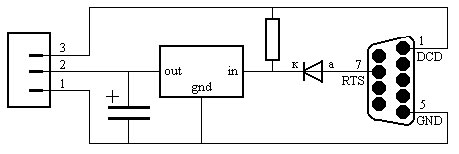
\includegraphics[width=8cm]{26_lirc_fig1}}
%\label{pic:fl1}
\caption{Схема инфракрасного приемника}
\end{figure}

\begin{figure}[ht]
\centering{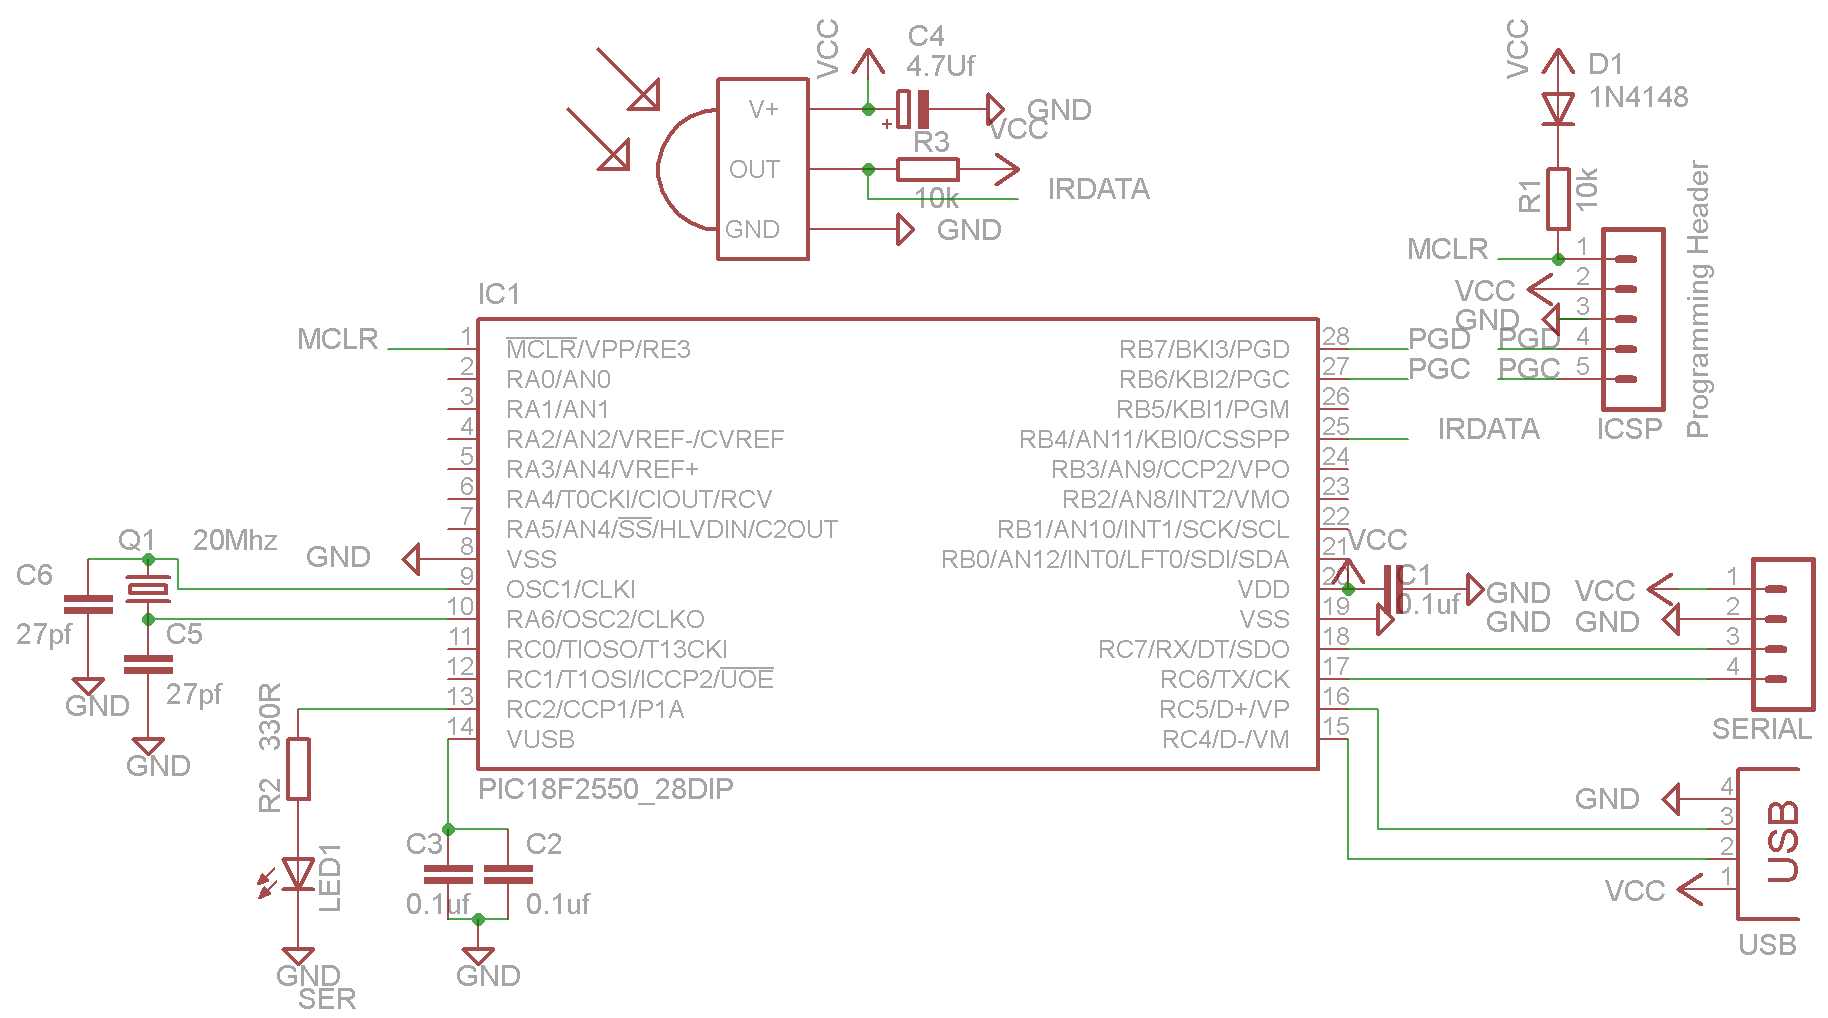
\includegraphics[width=8cm]{26_lirc_fig2}}
%\label{pic:fl1}
%\caption{Приложения по категориям}
\end{figure}

Такое решение является наиболее простым и доступным, однако, т.~к. COM-порт 
уже исчезающий вид интерфейса, более привлекательными выглядят
USB-приемники. Для его изготовления потребуется микроконтроллер.

Приемник базируется на микроконтроллере PIC18F2455, который может
работать с USB-портом и является меньшей и более дешевой версией
18F2550. Семейство 18F можно программировать при помощи универсального
PIC-программатора.

В состав пакета LIRC входят:
\begin{itemize}
	\item драйверы различных устройств (модули ядра)
	\item демон lircd, преобразующий ИК сигналы, полученные от драйвера, в стандартные сообщения, которые прикладные программы могут получить
через сокет 
\item демон lircmd, получающий сообщения от lircd и имитирующий мышь в X Windows
\item irexec "--- запуск программ по нажатию кнопки ДУ
\item irxevent "--- посылка X Windows сообщения по нажатию кнопки ДУ
\item irpty "--- псевдотерминал, запускающий программу и имитирущий нажатие клавиш клавиатуры
\end{itemize}
Кроме того, стоит упомянуть вспомогательные программы для отладки и настройки:
\begin{itemize}
	\item irrecord "--- утилита для записи сегналов пульта и создания lircd.conf
	\item irw "--- читает сообщения с сокета lircd и выдает на stdout; в качестве параметра можно указать имя сокета
	\item ircat "--- отладочная программа для конфигурационного файла ~/.lircrc; в качестве параметра указывается имя программы (точнее имя описывающей
её секции); по нажатию кнопки на пульте ДУ ircat выводит на stdout строку, привязанную к этой кнопке
\item mode2, smode2, xmode2 "--- осциллоскоп для инфракрасных сигналов
\item irsend "--- посылает команды на инфракрасные приемники (если позволяет оборудование)
\end{itemize}
В Linux существует множество приложений, направленных на централизованную работу с мультимедиа, например MythTV, Elisa,
XBMC. Однако, очевидно, что пульт может использоваться совместно с множеством других программных пакетов.

\end{document}



\documentclass[10pt, a5paper]{article}
\usepackage{pdfpages}
\usepackage{parallel}
\usepackage[T2A]{fontenc}
\usepackage{ucs}
\usepackage[utf8x]{inputenc}
\usepackage[polish,english,russian]{babel}
\usepackage{hyperref}
\usepackage{rotating}
\usepackage[inner=2cm,top=1.8cm,outer=2cm,bottom=2.3cm,nohead]{geometry}
\usepackage{listings}
\usepackage{graphicx}
\usepackage{wrapfig}
\usepackage{longtable}
\usepackage{indentfirst}
\usepackage{array}
\newcolumntype{P}[1]{>{\raggedright\arraybackslash}p{#1}}
\frenchspacing
\usepackage{fixltx2e} %text sub- and superscripts
\usepackage{icomma} % коскі ў матэматычным рэжыме
\PreloadUnicodePage{4}

\newcommand{\longpage}{\enlargethispage{\baselineskip}}
\newcommand{\shortpage}{\enlargethispage{-\baselineskip}}

\def\switchlang#1{\expandafter\csname switchlang#1\endcsname}
\def\switchlangbe{
\let\saverefname=\refname%
\def\refname{Літаратура}%
\def\figurename{Іл.}%
}
\def\switchlangen{
\let\saverefname=\refname%
\def\refname{References}%
\def\figurename{Fig.}%
}
\def\switchlangru{
\let\saverefname=\refname%
\let\savefigurename=\figurename%
\def\refname{Литература}%
\def\figurename{Рис.}%
}

\hyphenation{admi-ni-stra-tive}
\hyphenation{ex-pe-ri-ence}
\hyphenation{fle-xi-bi-li-ty}
\hyphenation{Py-thon}
\hyphenation{ma-the-ma-ti-cal}
\hyphenation{re-ported}
\hyphenation{imp-le-menta-tions}
\hyphenation{pro-vides}
\hyphenation{en-gi-neering}
\hyphenation{com-pa-ti-bi-li-ty}
\hyphenation{im-pos-sible}
\hyphenation{desk-top}
\hyphenation{elec-tro-nic}
\hyphenation{com-pa-ny}
\hyphenation{de-ve-lop-ment}
\hyphenation{de-ve-loping}
\hyphenation{de-ve-lop}
\hyphenation{da-ta-ba-se}
\hyphenation{plat-forms}
\hyphenation{or-ga-ni-za-tion}
\hyphenation{pro-gramming}
\hyphenation{in-stru-ments}
\hyphenation{Li-nux}
\hyphenation{sour-ce}
\hyphenation{en-vi-ron-ment}
\hyphenation{Te-le-pathy}
\hyphenation{Li-nux-ov-ka}
\hyphenation{Open-BSD}
\hyphenation{Free-BSD}
\hyphenation{men-ti-on-ed}
\hyphenation{app-li-ca-tion}

\def\progref!#1!{\texttt{#1}}
\renewcommand{\arraystretch}{2} %Іначай формулы ў матрыцы зліпаюцца з лініямі
\usepackage{array}

\def\interview #1 (#2), #3, #4, #5\par{

\section[#1, #3, #4]{#1 -- #3, #4}
\def\qname{LVEE}
\def\aname{#1}
\def\q ##1\par{{\noindent \bf \qname: ##1 }\par}
\def\a{{\noindent \bf \aname: } \def\qname{L}\def\aname{#2}}
}

\def\interview* #1 (#2), #3, #4, #5\par{

\section*{#1\\{\small\rm #3, #4. #5}}

\def\qname{LVEE}
\def\aname{#1}
\def\q ##1\par{{\noindent \bf \qname: ##1 }\par}
\def\a{{\noindent \bf \aname: } \def\qname{L}\def\aname{#2}}
}

\begin{document}
\title{GRID-технологии в исследованиях дымовой плазмы}
\author{Сподарец Д.В., Драган Г.С.\footnote{Одесса, Украина, Одесский национальный университет имени И.И.Мечникова, \url{m31@root-ua.com}}}
\date{}
\maketitle
\begin{abstract}
The paper describes the use of GRID systems and computer clusters for smoky plasma research. Offers insight into the experience of expanding the functionality of TERM software and hardware complex for GRID systems.
\end{abstract}
В экспериментах все чаще используют  вычислительные кластеры и GRID-системы. Связано это с тем, что количество информации, полученное в следствии проведения эксперимента с использованием современного измерительного оборудования, достаточно велико. Немаловажным фактом, который играет роль при выборе супперкомпьютеров для автоматизации исследований и обработки результатов, является уменьшение ошибки измерений, а также возможность использовать новые технологии диагностики, например, позволяющие наблюдать процессы в реальном времени.

Основной объект наших исследований --- дымовая плазма. Она является разновидностью низкотемпературной термической плазмы с конденсированной дисперсной фазой, образуется в продуктах сгорания топлива и состоит из газовой фазы с легкоионизируемой примесью атомов щелочного металла и конденсированной в виде частиц оксидов металлов и сажи \cite{spod1}.

Для проведения диагностики таких параметров дымовой плазмы, как температура газовой и конденсированной фаз, концентрации электронов и атомов, нами был разработан аппаратно"=программный комплекс TERM \cite{spod2}. В его основе лежат оптические методы диагностики плазмы, а программная часть построена на свободном программном обеспечении. Среди новых возможностей комплекса, которые уже реализованы или находятся на стадии реализации, можно отметить дополнение его собственным вычислительным кластером, адаптация для работы в GRID-системах, разработка механизмов проведения виртуальных экспериментов \cite{spod3}.

Комплекс TERM работает следующим образом:
\begin{enumerate}
	\item Экспериментально определяется температура газовой и конденсированной фаз, а также концентрация электронов и атомов в плазме.
	\item На основе теории дымовой плазмы и измеренных экспериментально параметров проводится расчёт заряда частиц, а также определяется функция распределения частиц по заряду.
	\item Полученные данные зарядов используются для определения пространственного концентрационного неравновесия и сил \linebreak диффузионно-дрейфового давления свободных носителей заряда на частицы. Основой для данных расчётов служит теория обобщённого потенциала.
	\item Значения сил диффузионно-дрейфового давления учитываются при  расчёте парного взаимодействия частиц, а также в уравнениях молекулярной динамики для дымовой плазмы.
	\item Результатом работы комплекса является моделирование 3D структур заряженных конденсированных частичек в плазме. Этот этап проводится с использованием GRID Украины.
\end{enumerate}
Базовой ОС комплекса является ALT Linux. Для захвата и обработки видеопотоков применяется библиотека компьютерного зрения OpenCV. В качестве инструментария, при проведении расчётов, задействованы Octave и Mathematica. Разработан ряд собственных специфических алгоритмов, например, для проведения анализа спектров излучения плазмы. 

При совмещении реального физического эксперимента и виртуального моделирования на базе GRID Украины, стало возможным более глубокое изучение влияния объёмных и поверхностных процессов, происходящих в области пространственного заряда конденсированной частицы, на кинетику и динамику дымовой плазмы.
\begin{thebibliography}{9}
	\bibitem{spod1}Dragan G.S., Malgota A.A. et al. // Proc. Sc. and Tech. Meet., Alma-Ata, USSR, October 25-31, 1982. – Inst. High Temp., Acad. Sci. of the USSR, 1984. – P. 191 – 192. 
	\bibitem{spod2} http://term.m31.org.ua
	\bibitem{spod3} Spodarets D.V., Dragan G.S. Method of Experimental Research of Long-Range Interactions in Smoky Plasmas // Book of Abstr. of the ICPDP 2011, Garmasch-Partenkirchen. Germany.: 2011. P. 74. 
\end{thebibliography}
\end{document}



\documentclass[10pt, a5paper]{article}
\usepackage{pdfpages}
\usepackage{parallel}
\usepackage[T2A]{fontenc}
\usepackage{ucs}
\usepackage[utf8x]{inputenc}
\usepackage[polish,english,russian]{babel}
\usepackage{hyperref}
\usepackage{rotating}
\usepackage[inner=2cm,top=1.8cm,outer=2cm,bottom=2.3cm,nohead]{geometry}
\usepackage{listings}
\usepackage{graphicx}
\usepackage{wrapfig}
\usepackage{longtable}
\usepackage{indentfirst}
\usepackage{array}
\newcolumntype{P}[1]{>{\raggedright\arraybackslash}p{#1}}
\frenchspacing
\usepackage{fixltx2e} %text sub- and superscripts
\usepackage{icomma} % коскі ў матэматычным рэжыме
\PreloadUnicodePage{4}

\newcommand{\longpage}{\enlargethispage{\baselineskip}}
\newcommand{\shortpage}{\enlargethispage{-\baselineskip}}

\def\switchlang#1{\expandafter\csname switchlang#1\endcsname}
\def\switchlangbe{
\let\saverefname=\refname%
\def\refname{Літаратура}%
\def\figurename{Іл.}%
}
\def\switchlangen{
\let\saverefname=\refname%
\def\refname{References}%
\def\figurename{Fig.}%
}
\def\switchlangru{
\let\saverefname=\refname%
\let\savefigurename=\figurename%
\def\refname{Литература}%
\def\figurename{Рис.}%
}

\hyphenation{admi-ni-stra-tive}
\hyphenation{ex-pe-ri-ence}
\hyphenation{fle-xi-bi-li-ty}
\hyphenation{Py-thon}
\hyphenation{ma-the-ma-ti-cal}
\hyphenation{re-ported}
\hyphenation{imp-le-menta-tions}
\hyphenation{pro-vides}
\hyphenation{en-gi-neering}
\hyphenation{com-pa-ti-bi-li-ty}
\hyphenation{im-pos-sible}
\hyphenation{desk-top}
\hyphenation{elec-tro-nic}
\hyphenation{com-pa-ny}
\hyphenation{de-ve-lop-ment}
\hyphenation{de-ve-loping}
\hyphenation{de-ve-lop}
\hyphenation{da-ta-ba-se}
\hyphenation{plat-forms}
\hyphenation{or-ga-ni-za-tion}
\hyphenation{pro-gramming}
\hyphenation{in-stru-ments}
\hyphenation{Li-nux}
\hyphenation{sour-ce}
\hyphenation{en-vi-ron-ment}
\hyphenation{Te-le-pathy}
\hyphenation{Li-nux-ov-ka}
\hyphenation{Open-BSD}
\hyphenation{Free-BSD}
\hyphenation{men-ti-on-ed}
\hyphenation{app-li-ca-tion}

\def\progref!#1!{\texttt{#1}}
\renewcommand{\arraystretch}{2} %Іначай формулы ў матрыцы зліпаюцца з лініямі
\usepackage{array}

\def\interview #1 (#2), #3, #4, #5\par{

\section[#1, #3, #4]{#1 -- #3, #4}
\def\qname{LVEE}
\def\aname{#1}
\def\q ##1\par{{\noindent \bf \qname: ##1 }\par}
\def\a{{\noindent \bf \aname: } \def\qname{L}\def\aname{#2}}
}

\def\interview* #1 (#2), #3, #4, #5\par{

\section*{#1\\{\small\rm #3, #4. #5}}

\def\qname{LVEE}
\def\aname{#1}
\def\q ##1\par{{\noindent \bf \qname: ##1 }\par}
\def\a{{\noindent \bf \aname: } \def\qname{L}\def\aname{#2}}
}

\begin{document}
\title{Свободное производство информации в постиндустриальном обществе}
\author{Елена Иванова\footnote{Москва, Россия, \url{http://coofeed.com}}, Дмитрий Костюк\footnote{Брест, Беларусь, \url{dmitriykostiuk@gmail.com}}}
\date{}
\maketitle
\begin{abstract}
The concept of postindustrial society is discussed in relation to free / open source software community-driven production. Its better correlation with Bell principles than classic information-as-a-good approach is shown. 
\end{abstract}

Концепция постиндустриализма в качестве следующей стадии социального развития приобрела широкую известность в 1970-х годах, когда Д. Беллом были сформулированы следующие положения \cite{ivanova1}, лежащие в его основе: главенствующая роль знаний в обществе (1), главенствующая роль производства не товаров, но услуг (2), университет как очаг производства новых знаний и инноваций (3). Исходно реализацию перечисленных принципов затрудняла дороговизна и малая эффективность коммуникации между специалистами. Ставшая популярной в 90-х концепция информационного общества \cite{ivanova2} включила в себя построение глобального информационного пространства с использованием новых компьютерных технологий, и таким образом в значительной степени снизила коммуникационный барьер за счет на порядок более эффективного удаленного взаимодействия.

Популярное толкование положения о информации и знаниях, как главном продукте производства, рассматривает поточное производство информации как товара в рамках сервисной (т. е. ориентированной на рынок услуг) экономики. В определенном смысле первый и третий из сформулированных Беллом признаков постиндустриального общества рассматриваются в качестве сателлитов положения о примате производства услуг. 

Производство информации более прибыльно в сравнении с материальным производством, так как достаточно изготовить первоначальный образец, а затраты на копирование несущественны. Но эти же свойства информации делают ее неудобным товаром с точки зрения традиционных экономических отношений. Когда под предоставлением услуг понимается торговля информацией или сдача информации в аренду, приходится изобретать искусственные ограничительные механизмы. Необходима развитая юридическая защита прав интеллектуальной собственности. Права на информацию, которые подлежат юридической защите, должны носить монопольный характер (это является не только необходимым условием для превращения информации в товар, но и позволяет извлекать монопольную прибыль, увеличивая рентабельность постиндустриальной экономики). Необходимо огромное количество потребителей, которые готовы платить за информацию, предоставляемую в данной ограниченной форме.

Однако возрастание числа людей, занятых информационными технологиями, коммуникациями и производством информационных продуктов и услуг "--- людей, основным «средством производства» которых является не оборудование работодателя, а их собственная квалификация \cite{ivanova2} "--- вносит в данный подход коррективы. В результате, существенная часть членов общества оказывается неудовлетворенной накладываемыми на информационный продукт искусственными ограничениями, делающими его использование менее удобным и осознает, что сверхприбыли поставщиков информационного продукта противоречат интересам их, как потребителей. Такая группа имеет средства производства для коллективного воссоздания аналога и сетевую инфраструктуру, позволяющую добиться предсказанной апологетами постиндустриализма быстрой самоорганизации творческих коллективов для решения конкретных задач, а ее представители готовы воспринимать в качестве опосредованного источника прибыли дополнительные факторы, такие как рост личного профессионализма и профессиональную репутацию.

Наиболее ярко на сегодняшний день данное явление проявляется в сфере свободного программного обеспечения. Группы специалистов, неудовлетворенные ситуацией на рынке, объединяются, выделяя часть своего свободного времени (являющегося в постиндустриальном обществе оцениваемым ресурсом) для создания равноценного программного продукта, свободного от искусственных ограничений, связанных с интеллектуальной монополией \cite{ivanova3} какого-либо производителя. В качестве страховки интересов потребителей такой продукт часто оснащается собственными лицензионными ограничениями, направленными против его возможной монополизации.
В рамках сформулированной концепции информационного общества данное явление можно рассматривать как массовое коллективное инвестирование, базирующееся на совладении материальными и нематериальными активами (crowd funding). Характерно также, что первоначальными источниками появления свободных программ являлись университеты, в полном соответствии с одним из сформулированных Беллом положений.

Модели бизнеса, построенные вокруг таких продуктов, хорошо укладываются в постиндустриальную модель, предоставляя коммерческие услуги по сопровождению и/или доработке продукта, а также доступ к продукту (консолидированному и обслуживаемому централизованно на мощных вычислительных станциях) в рамках облачных вычислений и технологии Software-As-Service (приложение как услуга).

Явление коллективного производства свободно распространяемых информационных продуктов претерпевает некоторые эволюционные изменения, связанные с большей доступностью для потребителя и проникновением в смежные области, примером чему служат коллективное создание высококачественного энциклопедического контента википедии и родственных проектов, а также активизация на рынке средств мобильной связи. В частности, идеи объединения функциональности сотового телефона и карманного персонального компьютера появились практически сразу после появления первых карманных персональных компьютеров в начале 90-х. Наличие полнофункциональной операционной системы делает смартфоны и коммуникаторы более привлекательными в глазах большинства пользователей. Современные телефоны прекрасно справляются со многими задачами, выходящими за рамки телефонных: работа с электронной почтой, просмотр текстовых документов и электронных таблиц, работа с планировщиком задач и многими другими. Однако резкий рост популярности смартфонов произошел одновременно с развитием инфраструктуры открытой операционной системы Android \cite{ivanova4}.
Аналогичным по своей сути направлением эволюции в компьютерных технологиях является децентрализация, примером которой могут служить файловый обмен (торенты), электронные системы платежей, такие как BitCoin \cite{ivanova5}, распределенные социальные сети.

\newpage\begin{thebibliography}{9}
	\bibitem{ivanova1} Д. Белл. Грядущее постиндустриальное общество. М., Академия, 1999.
	\bibitem{ivanova2} Постиндустриальное общество. \url{http://ru.wikipedia.org}  
	\bibitem{ivanova3} Л. Лессиг. Свободная культура. \url{http://www.gumer.info/bibliotek_Buks/Culture/lessig/index.php}
	\bibitem{ivanova4} Source: Gartner (May 2011) \url{http://www.gartner.com/it/page.jsp?id=1689814}
	\bibitem{ivanova5} BitCoin --- анархическая пиринговая криптовалюта. \url{http://blogerator.ru/page/bitcoin}
\end{thebibliography}
\end{document}



\documentclass[10pt, a5paper]{article}
\usepackage{pdfpages}
\usepackage{parallel}
\usepackage[T2A]{fontenc}
\usepackage{ucs}
\usepackage[utf8x]{inputenc}
\usepackage[polish,english,russian]{babel}
\usepackage{hyperref}
\usepackage{rotating}
\usepackage[inner=2cm,top=1.8cm,outer=2cm,bottom=2.3cm,nohead]{geometry}
\usepackage{listings}
\usepackage{graphicx}
\usepackage{wrapfig}
\usepackage{longtable}
\usepackage{indentfirst}
\usepackage{array}
\newcolumntype{P}[1]{>{\raggedright\arraybackslash}p{#1}}
\frenchspacing
\usepackage{fixltx2e} %text sub- and superscripts
\usepackage{icomma} % коскі ў матэматычным рэжыме
\PreloadUnicodePage{4}

\newcommand{\longpage}{\enlargethispage{\baselineskip}}
\newcommand{\shortpage}{\enlargethispage{-\baselineskip}}

\def\switchlang#1{\expandafter\csname switchlang#1\endcsname}
\def\switchlangbe{
\let\saverefname=\refname%
\def\refname{Літаратура}%
\def\figurename{Іл.}%
}
\def\switchlangen{
\let\saverefname=\refname%
\def\refname{References}%
\def\figurename{Fig.}%
}
\def\switchlangru{
\let\saverefname=\refname%
\let\savefigurename=\figurename%
\def\refname{Литература}%
\def\figurename{Рис.}%
}

\hyphenation{admi-ni-stra-tive}
\hyphenation{ex-pe-ri-ence}
\hyphenation{fle-xi-bi-li-ty}
\hyphenation{Py-thon}
\hyphenation{ma-the-ma-ti-cal}
\hyphenation{re-ported}
\hyphenation{imp-le-menta-tions}
\hyphenation{pro-vides}
\hyphenation{en-gi-neering}
\hyphenation{com-pa-ti-bi-li-ty}
\hyphenation{im-pos-sible}
\hyphenation{desk-top}
\hyphenation{elec-tro-nic}
\hyphenation{com-pa-ny}
\hyphenation{de-ve-lop-ment}
\hyphenation{de-ve-loping}
\hyphenation{de-ve-lop}
\hyphenation{da-ta-ba-se}
\hyphenation{plat-forms}
\hyphenation{or-ga-ni-za-tion}
\hyphenation{pro-gramming}
\hyphenation{in-stru-ments}
\hyphenation{Li-nux}
\hyphenation{sour-ce}
\hyphenation{en-vi-ron-ment}
\hyphenation{Te-le-pathy}
\hyphenation{Li-nux-ov-ka}
\hyphenation{Open-BSD}
\hyphenation{Free-BSD}
\hyphenation{men-ti-on-ed}
\hyphenation{app-li-ca-tion}

\def\progref!#1!{\texttt{#1}}
\renewcommand{\arraystretch}{2} %Іначай формулы ў матрыцы зліпаюцца з лініямі
\usepackage{array}

\def\interview #1 (#2), #3, #4, #5\par{

\section[#1, #3, #4]{#1 -- #3, #4}
\def\qname{LVEE}
\def\aname{#1}
\def\q ##1\par{{\noindent \bf \qname: ##1 }\par}
\def\a{{\noindent \bf \aname: } \def\qname{L}\def\aname{#2}}
}

\def\interview* #1 (#2), #3, #4, #5\par{

\section*{#1\\{\small\rm #3, #4. #5}}

\def\qname{LVEE}
\def\aname{#1}
\def\q ##1\par{{\noindent \bf \qname: ##1 }\par}
\def\a{{\noindent \bf \aname: } \def\qname{L}\def\aname{#2}}
}

\begin{document}
\title{Голос спонсора: SaM Solutions}
%\author{}
\date{}
\maketitle

Компания SaM Solutions выступает в роли системо-образующего спонсора конференции Linux Vacation Eastern Europe с момента рождения LVEE в 2005 году и на протяжении всех лет её проведения. 

Сложившаяся корпоративная практика не случайна. Продукты и решения, задействующие Linux и другие Free/Open Source Software проекты, составляют заметную часть пакета разработок SaM Solutions. Кадровая политика компании направлена на поощрение профессионального развития своих сотрудников, организацию их эффективного отдыха и привлечение хорошо мотивированных кандидатов к работе на компанию. Формат конференции LVEE успешно позволяет решать все три задачи. 

Одним из подразделений компании является отдел Linux и \linebreak Embbeded. Специалисты компании на протяжении десятилетий работают с СПО. Компанией реализован ряд проектов по адаптации ОС GNU/Linux для работы в различных устройствах, построенных на таких платформах как ARM, PowerPC, x86, MIPS. В последние годы "--- на ведущие позиции выходит разработка управляющего ПО для серверов Enterprise-класса, от низкоуровнего BMC Firmware на основе Linux до высокоуровневых систем контроля виртуализации и графических интерфейсов управления, от прошивок устройств хранения данных до BSP интегрированных плат для разработчика. Надёжность, качество и широкая функциональность множества свободных проектов позволяет строить нам системы любого уровня и сложности, опираясь на высококачественные готовые компоненты.

В рамках направления Linux и Embedded успешно выполнены проекты для таких знаковых заказчиков, как  Novell/SUSE, Fujitsu Technology Solutions  и осуществляется партнёрство с компаниями IBM и Oracle/Sun в области Open Source решений.

Мы разрабатываем, модифицируем и адаптируем различное свободное программное обеспечение для наших заказчиков, но не забываем и о своих нуждах "--- наши сотрудники используют в своей работе существующие програмные продукты и вносят вклад в их развитие. Часть внутренней инфраструктуры, а именно интранет-сеть компании, тестовые стенды отдела контроля качества, рабочие места сотрудников профильных подразделений "--- также работает под управлением СПО (серверные и десктопные платформы GNU/Linux и FreeBSD). 

В минувшем году, в рамках реорганизации, был разработан долгосрочный план развития направления Linux и Embedded в SaM Solutions. В нём впервые были кодифицированы уже имеющиеся внутренние неофициальные практики по взаимодействию с commu"=nity-based проектами. В частности разработаны меры и правила по
\begin{itemize}
  \item возврата изменений в родительские проекты (upstreaming);
  \item вхождения в состав постоянных разработчиков активно используемых нами FOSS-компонентов;
  \item публикации сообщений об ошибках (bug reporting);
  \item участия и помощи в организации community events;
  \item стимуляции докладов и участия в технических конференциях.
\end{itemize}
И план немедленно начал претворяться в жизнь.

Силами отдела организовано внутреннее обучение сотрудников на регулярной
основе. Был прочтен и опубликован курс по TDD. По согласованию с автором
опубликован курс Debian/Ubuntu Packaging (видео, презентация и исходные
тексты презентации в \LaTeX).  Были организованы и проведены курсы по
обучению QA специалистов для направления Embeded Linux. Проведено
практическое занятие по основам виртуализации и эмуляции, организована
лекция по вопросу профилирования и оптимизации Ruby-кода, лекция о
High-availability кластерах и направлении развития технологии. Кроме того,
проводился семинар по Video4Linux2. Для создания и обучения кадрового
резерва на ближайшее будущее запланированы постоянно действующие внутренние
проекты в области Embedded Linux, результаты которых также запланированы к
публикации.

Визиты представительных делегаций на Embedded World 2012 и Linux Con Europe/Embedded LinuxCon Europe 2011 обогатили нас новыми идеями, куда можно
двигаться дальше и что сейчас актуально. А выступления на Software
Engineering Forum for Students, круглом столе по СПО в рамках TIBO-2012
и LVEE Winter 2012 позволили поделиться опытом с
заинтересованными сторонами.

В апреле состоялась Ганноверская промышленная ярмарка \linebreak (Hannover Messe
2013). Компания SaM Solutions была представлена отдельным стендом, на
котором демонстрировались наработки в области встроенного и системного ПО
на базе OS Linux. Идея «умного» дома вызвала неподдельный интерес у
посетителей стенда.

При поддержке SaM Solutions, с декабря 2011 года возобновились регулярные встречи Minsk Linux Users Groups, под названием <<Линуксовка в SaM Solutions>>. Техническое оснащение линуксовок и открытый формат встреч позволил им практически мгновенно стать заметным дискуссионным клубом по широкому спектру вопросов, прямо или косвенно связанных с СПО. Свободная картография (OpenStreetMap), технологии виртуализации, минский \linebreak hackerspace, Linux Mobile, бойкот Голливудской продукции, systemd, загрузчик u-boot, белорусская локализация GNOME --- это только часть тем, поднятых за последние линуксовки.

Быстрые и положительные изменения, как внутри компании SaM Solutions, так и в экосфере СПО (и Linux в частности) наполняют нас уверенностью, что направление движения выбрано верно.

\begin{figure}[h!]
\centering

\includegraphics[height=11.8cm]{48_spons_sams.pdf}
\end{figure}
\end{document}



\documentclass[10pt, a5paper]{article}
\usepackage{pdfpages}
\usepackage{parallel}
\usepackage[T2A]{fontenc}
\usepackage{ucs}
\usepackage[utf8x]{inputenc}
\usepackage[polish,english,russian]{babel}
\usepackage{hyperref}
\usepackage{rotating}
\usepackage[inner=2cm,top=1.8cm,outer=2cm,bottom=2.3cm,nohead]{geometry}
\usepackage{listings}
\usepackage{graphicx}
\usepackage{wrapfig}
\usepackage{longtable}
\usepackage{indentfirst}
\usepackage{array}
\newcolumntype{P}[1]{>{\raggedright\arraybackslash}p{#1}}
\frenchspacing
\usepackage{fixltx2e} %text sub- and superscripts
\usepackage{icomma} % коскі ў матэматычным рэжыме
\PreloadUnicodePage{4}

\newcommand{\longpage}{\enlargethispage{\baselineskip}}
\newcommand{\shortpage}{\enlargethispage{-\baselineskip}}

\def\switchlang#1{\expandafter\csname switchlang#1\endcsname}
\def\switchlangbe{
\let\saverefname=\refname%
\def\refname{Літаратура}%
\def\figurename{Іл.}%
}
\def\switchlangen{
\let\saverefname=\refname%
\def\refname{References}%
\def\figurename{Fig.}%
}
\def\switchlangru{
\let\saverefname=\refname%
\let\savefigurename=\figurename%
\def\refname{Литература}%
\def\figurename{Рис.}%
}

\hyphenation{admi-ni-stra-tive}
\hyphenation{ex-pe-ri-ence}
\hyphenation{fle-xi-bi-li-ty}
\hyphenation{Py-thon}
\hyphenation{ma-the-ma-ti-cal}
\hyphenation{re-ported}
\hyphenation{imp-le-menta-tions}
\hyphenation{pro-vides}
\hyphenation{en-gi-neering}
\hyphenation{com-pa-ti-bi-li-ty}
\hyphenation{im-pos-sible}
\hyphenation{desk-top}
\hyphenation{elec-tro-nic}
\hyphenation{com-pa-ny}
\hyphenation{de-ve-lop-ment}
\hyphenation{de-ve-loping}
\hyphenation{de-ve-lop}
\hyphenation{da-ta-ba-se}
\hyphenation{plat-forms}
\hyphenation{or-ga-ni-za-tion}
\hyphenation{pro-gramming}
\hyphenation{in-stru-ments}
\hyphenation{Li-nux}
\hyphenation{sour-ce}
\hyphenation{en-vi-ron-ment}
\hyphenation{Te-le-pathy}
\hyphenation{Li-nux-ov-ka}
\hyphenation{Open-BSD}
\hyphenation{Free-BSD}
\hyphenation{men-ti-on-ed}
\hyphenation{app-li-ca-tion}

\def\progref!#1!{\texttt{#1}}
\renewcommand{\arraystretch}{2} %Іначай формулы ў матрыцы зліпаюцца з лініямі
\usepackage{array}

\def\interview #1 (#2), #3, #4, #5\par{

\section[#1, #3, #4]{#1 -- #3, #4}
\def\qname{LVEE}
\def\aname{#1}
\def\q ##1\par{{\noindent \bf \qname: ##1 }\par}
\def\a{{\noindent \bf \aname: } \def\qname{L}\def\aname{#2}}
}

\def\interview* #1 (#2), #3, #4, #5\par{

\section*{#1\\{\small\rm #3, #4. #5}}

\def\qname{LVEE}
\def\aname{#1}
\def\q ##1\par{{\noindent \bf \qname: ##1 }\par}
\def\a{{\noindent \bf \aname: } \def\qname{L}\def\aname{#2}}
}

\begin{document}
\title{Голос спонсора: EPAM Systems}
%\author{}
\date{}
\maketitle

Компания EPAM Systems не первый год является спонсором международной конференции разработчиков и пользователей свободного программного обеспечения LVEE (Linux Vacation / Eastern Europe). Этот год также не стал исключением. Пожалуй, LVEE является самым значимым событием для русскоязычных разработчиков и тестировщиков Open Source. Каждое лето здесь встречаются начинающие специалисты и «ветераны»"=разработчики из десятка стран для обмена опытом и общения на профессиональные темы. Наши специалисты также активно участвуют в данной конференции: в качестве докладчиков и организаторов/волонтёров. Это уникальная в своём роде конференция, и именно поэтому EPAM Systems очередной раз принимает участие в LVEE в качестве спонсора.


EPAM Systems "--- одна из крупнейших компаний"=поставщиков\linebreak услуг в области разработки программного обеспечения и решений на территории СНГ и Центральной и Восточной Европы. Созданная в 1993 году, сегодня она имеет представительства в 12 странах мира, в штате работают более 9 тыс. сотрудников, из которых более 3 тыс. "--- в Беларуси. Рост компании обеспечивается за счет собственных обучающих программ и передаче опыта от больших специалистов до начинающих разработчиков. Компания EPAM Systems выполняет проекты более чем в 30 странах мира. Основные направления деятельности: разработка, тестирование, сопровождение и поддержка заказного программного обеспечения и бизнес"=приложений, а также ИТ"=консалтинг с учетом отраслевой специфики бизнеса.

Наша компания участвует в проектах с такими крупными, хорошо известными заказчиками как Google, Novell, Infoblox, Parallels, 10Gen и др., так и с небольшими, в том числе и с начинающими свой путь в софтверном бизнесе.


К примеру, для Infoblox была реализована связка между WebUI с BIND и DHCP. Для этого был разработан комплекс решений под управлением Shell и Python скриптов, а также механизм позволяющий вносить правки в BIND и DHCP на языке C. Также был разработан развернутый функционал, автоматизирующий инсталляцию новых устройств и их эксплуатацию, что позволяет значительно упростить управление данными. Встроенный Web"=интерфейс позволяет разворачивать, управлять сервисами DNS, DNSSEC, DHCP, IPAM, устанавливать новые версии ПО, архивировать и восстанавливать из архивов необходимые данные, восстанавливать их после аварии, проводить мониторинг сети и создавать отчеты без необходимости обращения к командной строке.


Еще одним решением, реализованным для компании Infoblox, являлся программный продукт, позволяющий контролировать сетевые изменения, таким образом, облегчая идентификацию трудноуловимых проблем конфигурации и соответствие требованиям. Вместо того чтобы просто регистрировать изменения, система использует внесенную информацию для проверки, анализа и автоматической обработки сетевых изменений. Благодаря инновационной, квалифицированной, глубокой технике логического анализа, программа изолирует проблемы исправности и конфигурации до того, как они могут вызвать более серьезные сбои.


Разработанная для анализа сложных сетей система изучает сеть, собирает ключевую информацию, применяет встроенную технику логического анализа и создает оценку исправности сети и список проблем, требующих принятие мер для улучшения качества работы сети.


Правильное использование свободного ПО в разработках сокращает и расходы на покупку лицензионных программ, и трудозатраты при создании коммерческого ПО. Немалую роль для достижения превосходного результата играет привлечение к разработке опытных специалистов. LVEE способствует появлению таких специалистов, развитию их навыков и расширению кругозора. Хотелось бы пожелать участникам конференции интересных проектов и максимум пользы от участия в LVEE.


\end{document}



\documentclass[10pt, a5paper]{article}
\usepackage{ucs}
\usepackage[utf8]{inputenc}
\usepackage[T2A]{fontenc}
\usepackage[english, russian]{babel}
\usepackage{hyperref}
\usepackage{geometry}
\usepackage{graphicx}
\frenchspacing
\begin{document}
\title{Голос спонсора: Ciklum}
%\author{}
\date{}
\maketitle
\begin{figure}[ht]
\centering{
\includegraphics[width=12cm]{51_spons_ciklum1}}
%\label{pic:fl1}
%\caption{Схема инфракрасного приемника}
\end{figure}

Ciklum is a Danish innovative IT outsourcing company specializing in nearshore software development. 
Established in 2002, Ciklum employs more than 1200+ IT specialists worldwide with more than 130+ current clients own development teams. Ciklum has pioneered a unique business model in Ukraine where employees have direct communication with the client and are equal to clients` home-based colleagues. In Ciklum we are working on the development of different kind of projects: from cross-platform end-user applications to multifunctional B2B scalable solutions.

What Ciklum offers to developers?
\begin{itemize}
\item Variety of knowledge sharing and training opportunities within Ciklum Knowledge Exchange community
\item A lot of various technical seminars
\item Unique working environment where you communicate and work directly with international businesses
\item Possibility to work in a big and successful company
\item Competitive salary
\item Career and professional growth 
\item Long-term employment with 20 working-days paid vacation and other social benefits 
\item State of the art, cool, centrally located offices with warm atmosphere which creates really good working conditions
\end{itemize}

Ciklum has four development offices in the four largest cities in Ukraine \& Belarus (Kyiv, Minsk, Kharkiv, Dnipropetrovsk, Donetsk) and two development offices in Pakistan (Lahore, Islamabad), as well as representative offices in Denmark, Sweden, United Kingdom, Switzerland, Germany and the Netherlands. 

Join Ciklum and «Cross the Borders» together with us!

\begin{figure}[hb]
\centering{
\includegraphics[width=12cm]{51_spons_ciklum2}}
%\label{pic:fl1}
%\caption{Схема инфракрасного приемника}
\end{figure}

\end{document}



\documentclass[10pt, a5paper]{article}
\usepackage{pdfpages}
\usepackage{parallel}
\usepackage[T2A]{fontenc}
\usepackage{ucs}
\usepackage[utf8x]{inputenc}
\usepackage[polish,english,russian]{babel}
\usepackage{hyperref}
\usepackage{rotating}
\usepackage[inner=2cm,top=1.8cm,outer=2cm,bottom=2.3cm,nohead]{geometry}
\usepackage{listings}
\usepackage{graphicx}
\usepackage{wrapfig}
\usepackage{longtable}
\usepackage{indentfirst}
\usepackage{array}
\newcolumntype{P}[1]{>{\raggedright\arraybackslash}p{#1}}
\frenchspacing
\usepackage{fixltx2e} %text sub- and superscripts
\usepackage{icomma} % коскі ў матэматычным рэжыме
\PreloadUnicodePage{4}

\newcommand{\longpage}{\enlargethispage{\baselineskip}}
\newcommand{\shortpage}{\enlargethispage{-\baselineskip}}

\def\switchlang#1{\expandafter\csname switchlang#1\endcsname}
\def\switchlangbe{
\let\saverefname=\refname%
\def\refname{Літаратура}%
\def\figurename{Іл.}%
}
\def\switchlangen{
\let\saverefname=\refname%
\def\refname{References}%
\def\figurename{Fig.}%
}
\def\switchlangru{
\let\saverefname=\refname%
\let\savefigurename=\figurename%
\def\refname{Литература}%
\def\figurename{Рис.}%
}

\hyphenation{admi-ni-stra-tive}
\hyphenation{ex-pe-ri-ence}
\hyphenation{fle-xi-bi-li-ty}
\hyphenation{Py-thon}
\hyphenation{ma-the-ma-ti-cal}
\hyphenation{re-ported}
\hyphenation{imp-le-menta-tions}
\hyphenation{pro-vides}
\hyphenation{en-gi-neering}
\hyphenation{com-pa-ti-bi-li-ty}
\hyphenation{im-pos-sible}
\hyphenation{desk-top}
\hyphenation{elec-tro-nic}
\hyphenation{com-pa-ny}
\hyphenation{de-ve-lop-ment}
\hyphenation{de-ve-loping}
\hyphenation{de-ve-lop}
\hyphenation{da-ta-ba-se}
\hyphenation{plat-forms}
\hyphenation{or-ga-ni-za-tion}
\hyphenation{pro-gramming}
\hyphenation{in-stru-ments}
\hyphenation{Li-nux}
\hyphenation{sour-ce}
\hyphenation{en-vi-ron-ment}
\hyphenation{Te-le-pathy}
\hyphenation{Li-nux-ov-ka}
\hyphenation{Open-BSD}
\hyphenation{Free-BSD}
\hyphenation{men-ti-on-ed}
\hyphenation{app-li-ca-tion}

\def\progref!#1!{\texttt{#1}}
\renewcommand{\arraystretch}{2} %Іначай формулы ў матрыцы зліпаюцца з лініямі
\usepackage{array}

\def\interview #1 (#2), #3, #4, #5\par{

\section[#1, #3, #4]{#1 -- #3, #4}
\def\qname{LVEE}
\def\aname{#1}
\def\q ##1\par{{\noindent \bf \qname: ##1 }\par}
\def\a{{\noindent \bf \aname: } \def\qname{L}\def\aname{#2}}
}

\def\interview* #1 (#2), #3, #4, #5\par{

\section*{#1\\{\small\rm #3, #4. #5}}

\def\qname{LVEE}
\def\aname{#1}
\def\q ##1\par{{\noindent \bf \qname: ##1 }\par}
\def\a{{\noindent \bf \aname: } \def\qname{L}\def\aname{#2}}
}

\begin{document}
\title{Интервью с участниками:}
%\author{}
\date{}
\maketitle

По сложившейся традиции в сборник материалов включены интервью, взятые представителями оргкомитета у участников конференции: как сразу после LVEE 2010, так и перед началом LVEE 2011. Участники рассказывают о себе и своей работе, делятся планами, высказывают мнения по актуальным вопросам, волнующим сообщество. Кроме литературной записи доступны также и оригиналы "--- видео"=записи на сайте конференции.

\section{Николай Маржан, Киев, Украина (LVEE 2010)}
%\begin{figure}[ht]
%\centering{\includegraphics[width=4cm]{49_spons_altoros.jpg}}
%\end{figure}

{\noindent \bf Николай Маржан:} Я работаю в компании PortaOne. Вот уже 3.5 года. Мои обязанности "--- это релиз-инжиниринг и, на данный момент, обеспечение работы системы мониторинга, которую я разработал с нуля.

{\noindent \bf LVEE: А чем занимается компания?}

{\noindent \bf Н:} Мы разрабатываем свои VOIP"=решения, основной продукт это VOIP"=биллинг и, соответственно, все сопутствующие сервисы.

{\noindent \bf L: В своей работе вам приходится использовать свободное ПО?}

{\noindent \bf Н:} Конкретно в моей работе "--- да. Я это очень приветствую, и все свои наработки мы отдаем под той же лицензией (GPL) нашим клиентам. Т.~е. если клиент купил наше решение, мы отдаем исходные коды, а если там GPL "--- под ней же свои доработки.

{\noindent \bf L: А как вообще возникла твоя симпатия к свободному ПО?}

{\noindent \bf Н:} Трудно сказать. Проще вспомнить, как появилась симпатия к Unix-way. В 16 лет я написал свой собственный форум на perl. И после этого влюбился в Unix. 

Был тогда бесплатный хостинг \url{agava.ru}, и на нем были только PHP и perl. Я посмотрел на PHP и понял, что это не мое. А perl\ldots Не считаю себя в нем гуру, но он мне очень нравится. 

{\noindent \bf L: И так мир Unix просочился\ldots}

{\noindent \bf Н:} Через эту лазейку.

{\noindent \bf L: Сейчас тебе приходится вплотную заниматься системным администрированием?}

{\noindent \bf Н:} Как раз системное администрирование от меня ушло почти полностью, кроме отладки системы мониторинга, и 95\% времени я являюсь разработчиком. Занимаюсь релиз-инжинирингом, т.е. подготавливаю наш продукт к деплойменту. Готовлю инсталляционные диски, апгрейд-процедуры, в общем делаю все, чтоб деплоймент прошел как можно легче. 

{\noindent \bf L: А мониторинг?}

{\noindent \bf Н:} На прошлой работе я 50\% времени занимался разработкой системы мониторинга, и вот, на новой "--- решили использовать накопленный опыт и предложили написать ее полностью с нуля.

В маленьких компаниях мы идем от готовых решений к реализации. В PortaOne я смог отталкиваться от того, что нужно потребителю "--- в данном случае отделу технической поддержки "--- к тому, как это реализовать. Невзирая на сроки, ориентируясь исключительно на качество. Это была главная идея, и благодаря ей я смог реализовать все что было задумано, без недостатков моих ранних систем мониторинга.

{\noindent \bf L: И какое же свободное ПО было задействовано в процессе?}

{\noindent \bf Н:} Из свободного ПО был использован проект nagios, был использован транспорт nagios'а, а это отдельный проект. Были позаимствованы кое"=какие скрипты построения графиков. Но на данный момент nagios можно заменить буквально тремя тысячами строк кода на perl, он сейчас используется просто как планировщик заданий. Т.~е. разработка переросла стадию инфраструктуры, связывающей несколько проектов, и стала самостоятельным проектом.

{\noindent \bf L: За пределами работы ты, вероятно, тоже пользуешься свободным ПО?}

{\noindent \bf Н:} Да, на своем десктопе 3 года использовал FreeBSD, но потом неудачно купил ноутбук :). Так что пришлось поставить на него Ubuntu. И теперь она на всех моих машинах.

{\noindent \bf L: Переход с FreBSD дался легко?}

{\noindent \bf Н:} Настолько легко, что трудно даже представить (это ведь не наоборот). На самом деле я считаю себя скорее BSD-гуру, чем Linux. Я являюсь мэйнтейнером нескольких портов FreeBSD и посто ее люблю.

О портах\ldots На самом деле они исходят из моих потребностей по работе. Что"=то было нужно "--- сделал порт. А потом подготовил его для включения в мэйнстрим. Мы, как комьюнити, должны отдавть свою работу "--- иначе\ldots Иначе мы не достигнем вселенского счастья :). Если я отдам свою крупицу сообществу, кто"=то ей воспользуется.

\section{Наим Шафиев, Москва, Россия (LVEE 2010)}

%\begin{figure}[ht]
%\centering{\includegraphics[width=4cm]{49_spons_altoros.jpg}}
%\end{figure}

{\noindent \bf Наим Шафиев:} Я из Москвы, работаю в компании ECUmoney Limited, параллельно учусь. Я могу себя позиционировать как поборник свободного ПО в его истинном проявлении, полностью без несвободных лицензий. Интересуюсь perl, пишу на нем, иногда приходится работать и с PHP, и с Pithon, и, боже мой, даже с Delphi. 

Но на самом деле я придерживаюсь главной теории экономики, что разделение труда "--- это великое благо, потому что при разделении труда выделяются наиболее способные люди для определенных вещей, соответственно повышается общая производительность труда. Соответственно, мой основной язык программирования это perl, я на нем программирую с 2001 года, но плотно занялся года три назад, можно сказать, к нему возвратился. Почему это так? Надо сказать, что perl 2001 года был не очень хорош, особенно для web. Использование CGI-обработки приложений является не очень хорошим способом обработки. Оно слишком низкоуровневое. Просто на тот момент ничего больше не было. Тот же PHP был посто ужасен на самом деле "--- он ничего не поддерживал. Кстати, я доклад прочитал миенно по поводу модернистического perl [на LVEE 2010], там я указал некоторые базовые направления,по которым стоит развиваться и на что стоит смотреть.

{\noindent \bf L: А свободное ПО "--- это больше профессиональный интерес или личные предпочтения?}

{\noindent \bf Н:} Я пытаюсь пользоваться только открытыми решениями, начиная от видеокарт и заканчивая\ldots буквально всем. Т.~е. если под устройство отсутствуют свободные драйвера "--- я его не использую. По крайней мере, стараюсь: сейчас все"=таки приходится использовать Radeon, там над открытыми драйверами, насколько я знаю, сейчас работают всего два челоаека\ldots Что в принципе ужасно. 

О профессиональной деятельности. В ECUmoney Limited мы используем практически полностью открытый стек. Используется CentOS. Хотя у нас был сервер на RHEL, но я считаю, что нет смысла платить за поддержку, которую я могу выполнять сам. ECUmoney Limited "--- мое основное место работы "--- это проект, который занимается веб-деньгами. Это новозеландский банк, и он осуществляет все операции вплоть до депонирования и работы на бирже. Менеджмент находится в Москве, соответственно там же я и работаю. 

{\noindent \bf L: А вот эта строгая позиция в отношении свободного ПО и непримиримость к двойным стандартам "--- как она возникла?}

{\noindent \bf Н:} С детства интересовался экономикой, особенно политэкономией. В принципе очевидно, что любые патенты, ограничения, проприетарщина "--- это ограничения свободы, и за счет этого происходит ограничение развития человечества. Могу привести одну цитату. Билл Гейтс, человек, который до недавнего времени руководил самой большой компанией по разработке проприетарного ПО, говорил: <<Если бы патенты существовали в том виде, в каком они существуют сейчас "--- никакая индустриальная революция, которая полностью перевернула жизнь людей в Европе в XVII веке, не прошла бы>>.

Что касается Unix-way "--- в 2001 году я начал изучать computer science, прочитал одну американскую книжку про альтернативные операционные системы. Тогда найти диск с FreeBSD даже в Москве было довольно сложно, но я нашел и попытался его установить. С первого раза конечно же ничего не получилось.  И жесткий диск я стер (но это ничего, я отношусь к тем админам, которые все"=таки делают бэкапы). Пришлось распечатать весь хэндбук (он был реально огромный), и заставить свою бабушку, профессионально владеющую английским, его переводить. С переводом "--- это была особая тема\ldots  И вот так я потихонечку пересел на свободное ПО. Сначала это была FreeBSD, потом Mandrake, потом Fedora, была еще пара тестовых дистрибутивов. Писал даже свой дистрибутив для встраиваемых решений. А в конце остановился на Debian: решил, что раз они наиболее сильные поборники свободного ПО, стоит на нем остановиться.

{\noindent \bf L: А участие в свободных проектах?}

{\noindent \bf Н:} В perl есть такая вещь как CPAN, (аббревиатура от четырех безумных слов, которые я сейчас не смогу воспроизвести) "--- репозиторий свободных проектов. Я в CPAN-е, можете набрать \url{search.cpan.org/~naim/} и увидите мой проект. На самом деле у меня разработок довольно много, но часть я пока не выкладывал, они еще не готовы для релиза. Моя разработка AnyEvent Benchmark "--- это довольно удобный фреймворк для осуществления собственных HTTP и HTTPS"=тестинга, для тестирования SOAP и других вещей. Сейчас она в разработке, я сам ее использую, как и еще пара членов \url{moscow.pm.org/}.

{\noindent \bf L: А как ты оказался на LVEE?}

{\noindent \bf Н:} Это довольно сложно. Информация о LVEE несколько раз появлялась на \url{linux.org.ru}, а я на этом ресурсе с 2003 года. 
Первый раз хотел приехать еще в 2009 году\ldots Для меня оказалось просто шоком, что в Беларуси проводится настолько прогрессивное мероприятие, формат которого на мой взгляд может в чем"=то соперничать с FOSSCON, плюс уровень разработчиков довольно хороший. 

\section*{Михаил Шалаев, Мюнхен, Германия (LVEE 2010)}

%\begin{figure}[ht]
%\centering{\includegraphics[width=4cm]{49_spons_altoros.jpg}}
%\end{figure}

{\noindent \bf Михаил Шалаев:} Родом я из Харькова, с Украины. Работаю в фирме, которая находится в Германии, в Мюнхене, и называется GeNUA, сокращение от\ldots  как это по"=русски\ldots сервисы для юникс и нетворк администрэйшн.

{\noindent \bf L: Как появился ваш интерес к свободному ПО?}

{\noindent \bf М:} Ну, когда я был совсем маленьким еще, под стол проходил, меня мама привела на работу, где стояла СМ ЭВМ, на которой смурные дядьки гоняли BSD 2.9. Точнее, советскую версию его, Демос 2.0, который был сделан частично из BSD 2.9, частично из System 3, по"=моему. Понятное дело, с русификацией, с переписанными мануалами и всеми делами. И смурные бородатые дядьки рассказали мне, что это и есть на самом деле фри операционная система, распространяется не за деньги, а любой человек может приехать в Беркли, привезти с собой большую тэйпу, откатать на нее себе дистрибутив и поехать домой пользователем. Вот. И потом как-то получилось так, даже не помню как, что я пользовал разнообразные BSD, немножко баловался с 386 BSD, потом с NetBSD, а потом в 95-м году образовался проект OpenBSD, я в нем участвовал девелопером некоторое время, и вот так это все и происходило. И продолжает.

{\noindent \bf L:  Удается совмещать интерес к свободному ПО и к BSD-системам в частности с профессиональной деятельностью?}

{\noindent \bf М:} Какое-то время я работал сисадмином в разнообразных конторах, и мы использовали BSD"=системы для роутеров, серверов, DNS"=серверов, и в частности я участвовал в разработке пакет"=фильтров для OpenBSD в свое время, потому что работал в небольшом ISP, и мы занимались фильтрованием как раз. 

{\noindent \bf L: Получается, что ваш код есть в одном из самых надежных\ldots}

{\noindent \bf М:} И не только :)

{\noindent \bf L: Чем вы сейчас занимаетесь по работе?}

{\noindent \bf М:} Я работаю в конторе, в которой мы, опять же, делаем файрволы. В данный момент из OpenBSD, раньше это был BSDi, но BSDi загнулся. Собственно чем я занимаюсь, это починкой злобных бугов, которые вылазят под безумной нагрузкой, поскольку некоторые клиенты, которые используют наше железо\ldots Собственно железо это разнообразные PC, от маленьких совсем до многопроцессорных гробов. И при большой нагрузке как правило вылазят буги, которые никто никогда не видел. Тут неважно что использовать, Linux или FreeBSD, или OpenBSD, все равно эти буги будут вылазить, потому что то что мы делаем, скорее всего никто другой не делает. И собственно то, чем я занимаюсь "--- это починка ядер OpenBSD.  Кроме того что мы делаем файрволы, мы людям помогаем организовывать их нетворк на базе того, что у них уже есть, плюс того что они еще хотят "--- в частности, опять"=таки наши файрволы. Фирма по-моему около 15 лет существует, сертифицирована для использования в правительстве. Небольшая, порядка 100 чаловек, большинство девелоперов являются или являлись OpenBSD"=девелоперами. 

{\noindent \bf L: За последнее время отношение к свободному ПО сильно меняется? В сфере, если не конечных пользователей, то решений?}

{\noindent \bf М:} Насколько вижу я, конечным клиентам все равно, что оно и как оно. Их волнуют две вещи: делает ли оно, что должно, и сколько оно стоит. Ну а бюджетные организации даже не волнует, сколько оно стоит "--- их волнует, чтоб оно работало. А что лежит в основе? Есть вероятно в этом какая"=то маркетинговая цена, потому что все читают журналы, видят как все хорошо в мире свободного программного обеспечения, но в конечном итоге они не покупают продукт, основанный на Linux, или BSD, или еще на чем-нибудь, а то, что отвечает их нуждам. В частности, наши железяки покупают потому, что есть не так много альтернатив. Мы делаем не простой пакет"=фильтеринг, мы делаем и разборку протокола, и сканирование на вирусы, и все остальное.

{\noindent \bf L: Иными словами, эти системы выигрывают из"=за преимуществ?}

{\noindent \bf М:} Отчачти из"=за того что есть сорс"=код, который можно починить, если что. Потому что основная проблема с  коммерческими системами "--- чинить их невозможно. Или если хочешь сделать что"=то свое на их основе. С другой стороны, есть отрицательный вариант в плане фирм, использующих free software: не всегда они дают назад то, что наваяли, или с другой стороны вместо того чтобы самим ваять, они ждут пока кто"=нибудь сделает. В результате получается, что большие конторы наживаются на маленьких конторах, которые собственно занимаются разработкой. Но я думаю, это явление временное отчасти, потому что большие конторы в конечном итоге упрутся в то, что никто не делает то, что им нужно, и начнут делать это сами.

А про LVEE мне товарищи сказали. Общались с товарищем из Минска, думали, как бы так организовать, чтобы повстречаться. И я просто спросил, не бывает ли каких смешных конференций в Беларуси. Они сказали, есть такая конференция, даже смахивает на хакер"=кэмп, как их организуют в Европе, и я решил поинтересоваться: а как же оно там? Точнее, здесь, там-то я уже видел. 

{\noindent \bf L: И как оно здесь?}

{\noindent \bf М:} Хорошо. С поправкой на количество людей, типичное для Евросоюза, и на формат, как оно все проходит "--- вполне сопоставимо с тем, как оно проходит там. В частности небольшие организации такого рода тоже происходят, вот на рождество обычно. Один раз на рождество дядьки просто сняли трамвай длинный , <<колбасу>>, и гоняли его по Мюнхену, имели интернет по GSM"=у , загружались пивом на каждом углу, потому как места не было в трамвае, и так ездили целую ночь, вот был у них такой хакер"=эвент. Там же организовались у них выступления, там же ели, пили и всем остальным занимались. Небольшая для Европы организация, до ста человек их было, а народ где"=то похожий. Я так думаю, на подобных конференциях, или там симпозиумах, всегда есть люди, которые делают то же самое. Идея"=то простая: рассказать чего сам делаешь, послушать что другие делают, и кто"=то это все дело должен окучить, вне зависимости от страны и языка.

\section{Wolfgang Spraul, Гонконг}

В рамках LVEE 2010 было также взято онлайн"=интервью у генерального директора гонконгской компании"=стартапа ООО Sharism, известной своими разработками в области свободного аппаратного обеспечения (САО). Вопросы от имени LVEE, кроме отдельно оговоренных случаев, руководству Sharism задавал Максим Мельников.

{\noindent \bf Wolfgang Spraul:} Пожалуйста, обратите внимание: я считаю, что это интервью действительно очень важно для нас и САО. СПО-движение в России и странах бывшего СССР, таких как Беларусь, существует давно и является очень активным. К сожалению, таможенные пошлины в этих странах имеют достаточно жесткую историю, поэтому русским фанатам СПО тяжело принимать участие в САО"=движении. Но, я верю, что мы придем и сюда.

\subsection*{В общем:}

{\noindent \bf W:} Я, Wolfgang Spraul "--- борец за свободу :-) А если серьёзно, я инженер, который почувствовал, что <<железо>>, которое разрабатывается на тех же принципах, что и СПО, может быть намного более успешным, чем традиционное проприетарное <<железо>>. Мне 35 лет, я живу в Китае и пытаюсь сделать САО возможным, как в техническом плане, так и в плане бизнеса. И еще я питаю пристрастие к Starbucks.

{\noindent \bf L: Что есть <<Sharism>>? Что есть <<Qi"=hardware>>? Что есть <<Ben Nanonote>>?}

{\noindent \bf W:} Qi"=hardware "--- это свободное аппаратное обеспечение (единственное объединение проектов <<свободного железа>>, которое я знаю). А свободное <<железо>>, это <<железо>>, которое сделано на основе свободных знаний, с использованием тех же принципов, что и СПО. Это процесс: некоторые элементы, такие как чипы памяти NAND и ПЗУ, ЖКИ "--- не будут свободными ещё долго. Но, как минимум, мы начали работать над полностью свободным процессором с Milkymist project.

ООО Sharism "--- маленькая Гонконгская компания"=стартап с 5 сотрудниками. Мы производим свободное оборудование в Китае, а это означает, что мы делаем оборудование без вендорских залоченных модулей. Все наши знания и вся информация доступна, мы используем только легко заменяемые компоненты, только ПО под GPL"=лицензиями и т.~д. Мы работаем как OEM / ODM, так что теоретически можем создать любой продукт, но практически имеет смысл работать на стандартной технологической базе, в нашем случае "--- на основе процессоров Ignetic XBurst.

Мы можем делать такие устройства, как GPS, цифровые фоторамки, цифровые камеры, телефоны, даже датчики напряжения и влажности.

Ben Nanonote "--- переносной карманный компьютер, похожий на маленький электронный словарь. Вес "--- 126 грамм включая батарею. Он на 100\% работает под управлением СПО. В данный момент, например, на ядре Linux 2.6.32. Мы отправили все патчи в upstream ядра 2.6.34, так что, возможно, через несколько месяцев у нас будет ядро с kernel.org, на 100\% поддерживающие наше устройство. Характеристики "--- 366МГц, MIPS"=подобный процессор, 32 Мб ОЗУ, 3"=дюймовый экран, но отсутствуют usb"=хост, wifi, bluetooth.

{\noindent \bf L: Когда (и как?) вы решили организовать вашу компанию? Правы ли люди, которые называют вас <<fork"=ом>> OpenMoko?}

{\noindent \bf W:} Компания ООО Sharism появилась в ноябре 2009"=го, когда стало ясно, что другие маленькие компании будут заинтересованы присоединиться к проекту Qi"=САО, и нам захотелось иметь отдельную маленькую компанию как азиатского производителя.

Некоторые из нас в прошлом работали для OpenMoko, но САО "--- это новая идея, и я не думаю, что OpenMoko когда-либо будет участвовать в САО"=проектах.

\subsection*{Разработка свободного <<железа>>:}

{\noindent \bf L: Какая самая большая проблема в разработке открытого <<железа>>?}

{\noindent \bf W:} Поиск клиентов, которые понимают долгосрочную перспективу, покупают наше простое маленькое <<железо>> сегодня (такое как Ben Nanonote) и помогают нам в разработке СПО для этого устройства. На данный момент мы продали 800 Ben Nanonote.

Как открытое <<железо>> может приносить деньги?

Точно таким же образом, как и проприетарное "--- через продажу высококачественных аппаратов, создание сильного бренда, лояльность клиентов благодаря хорошему сервису и т.~д.

{\noindent \bf L: Можешь привести простые математические расчёты, как <<железная>> компания может быть успешной? Цена на \linebreak устройство, доход, количество проданных экземпляров, \linebreak  размер компании?}

Это очень сложно, потому что есть разовые расходы, и есть расходы на каждую единицу. Также очень важен потенциал зарабатывания денег на сервисах, мелочах, и т.~д.

Мы потратили около \$180~000 наличными, чтобы сделать первую 1~000 Ben Nanote. Итак, если мы продадим 1~000 за \$99, мы всё равно в минусе. Возможно, если получится продать 2~000 или 3~000, это будет выглядеть лучше.

{\noindent \bf L: СПО даёт возможность объединять разработки "--- новые устройства получают большую базу ПО с самого начала. А что открытость <<железа>> даёт <<железному>> стартапу?}

То же самое. Сейчас в мире <<железа>> многие вещи изобретаются снова и снова. Объединив усилия, всего можно добиться намного лучше, это позволит производить лучшие продукты за более выгодную цену и быстрее выходить на рынок. Огромная неэффективность <<железного>> мира может быть преодолена благодаря использованию философии нашей компании, Sharism :-)

\subsection*{ООО Sharism:}

{\noindent \bf L: Как много людей работает в компании? Кто вы в плане структуры компании и организации?}

{\noindent \bf W:} 5 работников на полный рабочий день. В такой маленькой команде мы все помогаем друг другу, структура размыта, мы все обладаем нашим уникальным опытом, который мы привносим в нашу команду.

{\noindent \bf L: Какую последнюю цель вы успешно достигли? Какая следующая?}

{\noindent \bf W:} Последняя достигнутая "--- продать 400 Ben Nanonote к концу марта, была успешно выполнена. Следующая "--- продать 1~000 Ben Nanonote к концу июля.

{\noindent \bf L: ПО очень важно. Как ПО разрабатывается в вашей компании?}

{\noindent \bf W:} В большинстве случаев мы полагаемся на сообщество СПО, у нас нет денег для оплаты разработки ПО. Сообщество OpenWRT было особенно полезным, теперь мы видим некоторый интерес со стороны Jlime и некоторых Debian"=разработчиков.

{\noindent \bf Daniel A. Nagy, ePoint System: Устройства какого типа (телефоны, планшеты, нетбуки?) вы планируете произвести в будущем? У вас есть прогнозный график выпуска?}

{\noindent \bf W:} Мы можем произвести что угодно на базе процессоров Ingenic XBurst. Мы изучаем расширенные NanoNote, GPS"=устройства, цифровые фоторамки, телефоны, программируемые FPGA-матрицы, а также датчики электричества и воды. Если вы хотите что-нибудь в этом роде, с минимальным количеством в 5~000 единиц или около того, мы готовы сделать это в стиле САО.

{\noindent \bf D: Насколько совместимыми друг с другом вы планируете делать свои устройства, с точки зрения как аппаратного, так и программного обеспечения?}

{\noindent \bf W:} Унификация очень важна. Чтобы оценить ее, мы сначала смотрим на наиболее сложные части, особенно в отношении программного обеспечения. Например, мы учитываем ядро Linux, дистрибутив OpenWrt и т.~д. Мы рассматриваем совместимость с точки зрения ПО. С точки зрения аппаратуры наиболее сложные части "--- процессор Ingenic XBurst и FPGA от Xilinx.

{\noindent \bf L: Получили ли вы какие-нить комментарии от больших компаний?}

{\noindent \bf W:} Ничего серьёзного.

\subsection*{<<Железо>>:}

{\noindent \bf D: Вопрос по поводу модульности: будет ли это неприемлемо дорогим, с точки зрения денег, времени жизни батареи или веса, сделать все части пригодными к использованию независимо друг от друга: экран, клавиатуру, тач"=скрин, модуль 3G и т.д., так чтобы они соединялись с материнской платой через USB (не обязательно через стандартные разъемы, хотя бы на уровне сигналов?}

{\noindent \bf W:} Модульность не работает. Аппаратная индустрия вкладывает значительные однократные инвестиции, чтобы добиться интеграции
и низкой стоимости устройств. Теоретически все можно интегрировать на одной кремниевой пластине.
Цена производства кремниевой пластины может быть всего около 50 центов, если не смотреть на огромные однократные вложения, необходимые чтобы достигнуть этого уровня интеграции. 

\subsection*{Ben Nanonote:}

{\noindent \bf L: Энергопотребление. Как долго он может работать?}

{\noindent \bf W:} Мы получаем отчёты от пользователей, говорящие о 6"=15 часах, в зависимости от нагрузки.

{\noindent \bf Richard\_Ferlow, \url{habrahabr.ru}: Что пользователь может делать со своим Nanonote?}

{\noindent \bf W:} Наш последний OpenWrt"=образ от 7 мая 2010. Что работает сейчас "--- это консольные приложения такие как vi или mutt, или музыкальный плеер GMU, сделанный на SDL (он может проигрывать только Ogg Vorbis, а не патентованный MP3).

Чтобы получить список OpenWRT-приложений и их статус в Ben Nanonote, можно посмотреть <<Приложения>> на сайте.

Также вы можете запускать дистрибутив Debian или JLiMe, который также с недавних пор поддерживает Ben Nanonote: \url{http://jlime.com/mw4/index.php/Faq_nanonote}.

Так или иначе, потребуется некоторое время, чтобы сделать приложения, которые действительно будут хорошо работать на устройстве, а не просто их собрать.

{\noindent \bf jeka1202, \url{habrahabr.ru}: Почему экран намного меньше верхней части Ben NN?}

{\noindent \bf threesixzero, \url{habrahabr.ru}: Будет ли следующий Nanonote иметь более высокое разрешение?}

{\noindent \bf W:} Экран стандартного размера, 3"=дюймовый TFT, обычно этот размер также может быть в цифровых камерах. Другой популярный размер "--- 3.5"=дюймовый, но он не вмещается в габариты устройства. 3.2"=дюймовые экраны существуют, но они редки и дороги, а цветные экраны специального размера совершенно недоступны для маленьких компаний, таких как мы. Когда мы ищем инновации, мы смотрим на СПО, свободные технологии в первую очередь. Что касается TFT в Ben Nanonote, это Ilitek ILI8960 drive IC, с открытой спецификацией.

Когда мы думаем над улучшением экрана, мы пытаемся найти лучший экран с таким же IC, или улучшенным (следующей версии) Ilitek drive IC.

Таким образом мы сможем быстрее использовать стабильную апстрим"=версию Linux"=драйвера. Если у нас будет возможность выбирать между новым экраном: один большой, полупрозрачный и т.~д., но с закрытыми спецификациями и проприетарным драйвером, или другой более простой, размером 2.8 дюйма, но с открытой спецификацией "--- мы выберем более простой ЖКИ"=экран. Мы изобретаем свободу, мы хотим получать радость от технологий и изменять их для наших клиентов без спросов и разрешений.

\section{Алексей Кондратенко, Минск, Беларусь (LVEE 2011)}

\begin{figure}[ht]
\centering{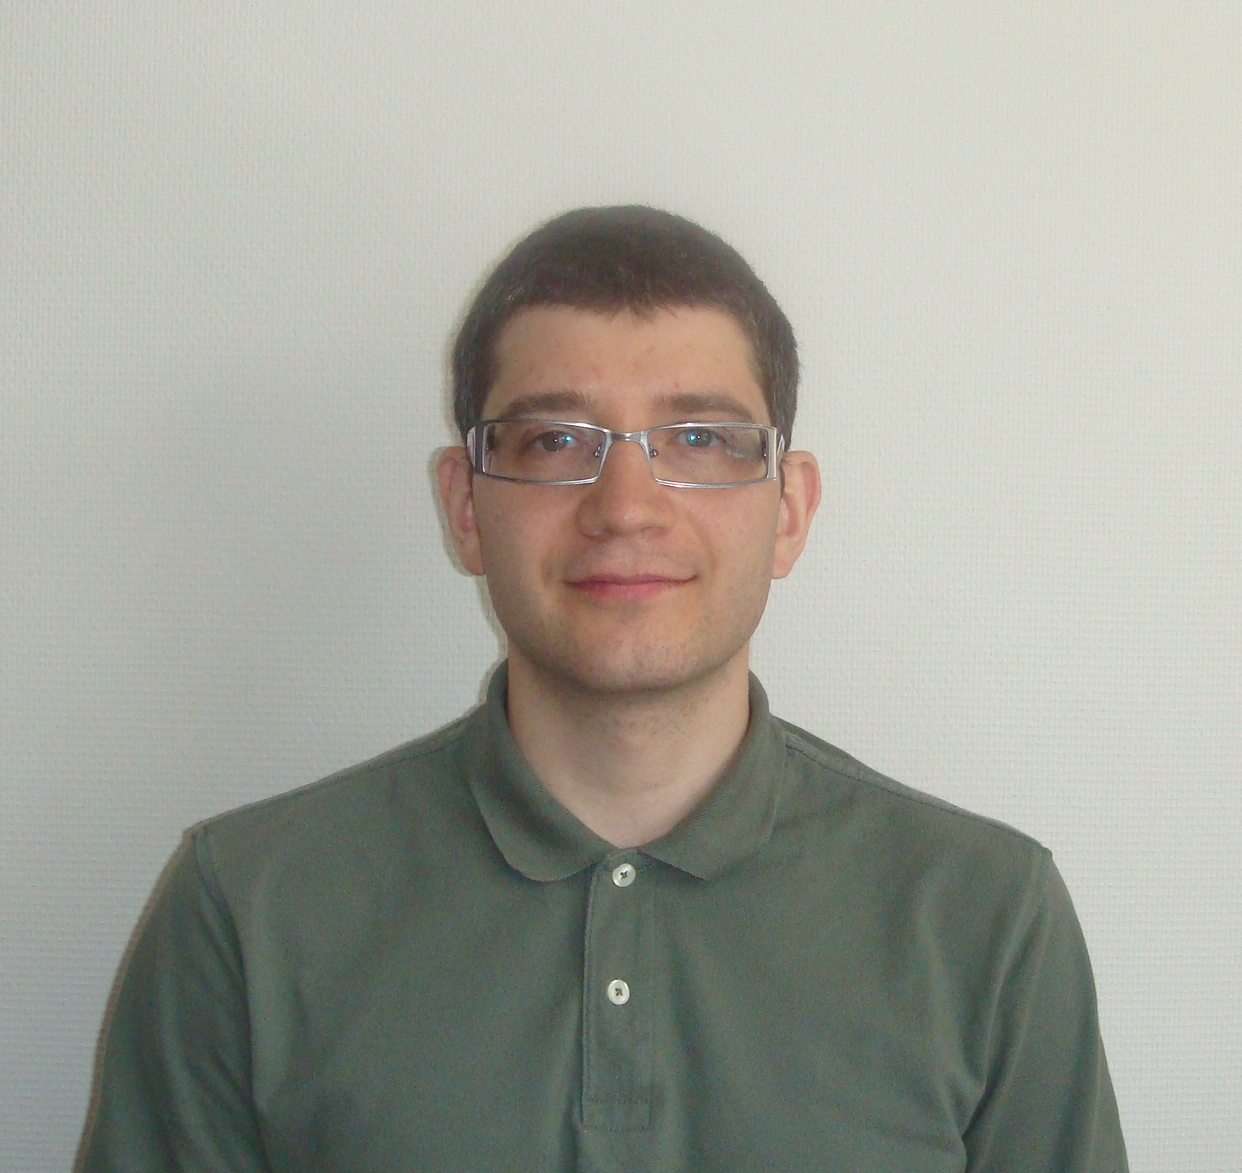
\includegraphics[width=4cm]{61_interv_2011_altoros.jpg}}
%\label{pic:fl1}
%\caption{Схема инфракрасного приемника}
\end{figure}

За несколько дней до конференции организаторы пообщались с одним из докладчиков LVEE-2011, Алексеем Кондратенко. Алексей "--- активный контрибьютор в open source"=проекты, в частности Membase (Couchbase), а также ведущий разработчик Альторос Девелопмент. Во время беседы он поделился своими мыслями о выборе лицензий, тенденциях open source"=проектов, недавней поездке в Кремниевую долину и дал несколько советов начинающим Linux"=разработчикам.

{\noindent \bf LVEE: Алексей, расскажи немного о себе.}

{\noindent \bf Алексей:} Программирую. Много.

{\noindent \bf L:  В каких свободных проектах ты принимал участие?}

{\noindent \bf A:} Мне довелось портировать один полупроприетарный драйвер программного модема в Linux 2.6. Я поучаствовал немного в разработке Ruby on Rails, а также написал замечательный навигатор по проекту и документации (gpicker). Но, разумеется, самое значительное, "--- это  мое участие в проекте Membase. И особенно приятно, что это работа за деньги, но над free software.
 
{\noindent \bf L:  Какой из этих проектов тебе наиболее интересен с профессиональной точки зрения?}

{\noindent \bf A:} В каждом проекте или проектике есть свои изюминки. Я считаю, что не бывает неинтересных задач. Бывают только неинтереснее решения. Я считаю, что очень важно научиться получать удовольствие от качественно сделанной работы. Тогда любая, даже самая тривиальная задача, будет приносить удовольствие. В компании, где я работаю, созданы именно такие условия для самореализации.

{\noindent \bf L:  Расскажи нам о своем мнении по поводу основных лицензий для распространения ПО. Сдерживают ли по"=твоему лицензионные ограничения развитие open source"=продуктов?}

{\noindent \bf A:} Два больших и очень различных класса "--- это copyleft и non-copyleft лицензии.

Первый класс представляют лицензии вроде GPL, LGPL и AGPL. Эти лицензии обеспечивают публичность модификаций. GPL, например, требует, чтобы параллельно с предоставлением готовой программы (оригинальной или модифицированной) предоставлялся доступ к исходным кодам. Это не позволяет всяким жадным корпорациям развивать свои закрытые форки. К сожалению, я был свидетелем того, как люди,  на мой взгляд неоправданно, опасаются этого класса лицензий. Я слышал, будто бы GPL"=код помешал покупке нескольких стартапов. Всем известно, что Android практически целиком избегает GPL (кроме неизбежного GPL для kernel).

Второй класс не накладывает copyleft"=ограничений. Он позволяет компаниям «наживаться» на своих закрытых версиях open source"=проектов. Хотя обычно скрывать код и форкать его не очень выгодно. Так что сторонники этого класса лицензий как правило упирают на большую либеральность. Сама возможность делать с кодом все что угодно "= большой плюс для них.

Конечно, copyleft versus non"=copyleft являются только одной гранью различия лицензий. Есть еще много всяких тонкостей, например, борьба против DRM и патентная волокита.

Выбор лицензии (или смена ее) может быть поводом для создания альтернативного проекта с более мягкой лицензией. Например, компания Apple полным ходом идет к отказу от GPL"=ного GCC в пользу основанного на LLVM набора компиляторов Clang. Сейчас они поставляют очень древние версии gcc, gdb и других частей gnu toolchain. Одной из причин является переход данных проектов на GPL версии 3. Также есть основания полагать, что Apple готовит альтернативу Samba, которая тоже перешла на GPL3.

 
{\noindent \bf L:  Поделись своими мыслями, за счёт чего идёт развитие open source"=проектов? В смысле финансовой стороны.}

{\noindent \bf A:} Есть разные модели зарабатывания денег на free software. В последнее время большее распространение получает модель, при которой клиенты покупают не сам софт, а подписку на поддержку. RedHat довольно успешно зарабатывает миллиарды в год на этой модели.

Но голый энтузиазм никогда не пропадет полностью. На github, например, можно найти кучу очень впечатляющих проектов, которые люди делают в свое личное время.


{\noindent \bf L:  Как ты считаешь, при сравнении open source"=проектов с коммерческими, в каком случае качество проигрывает и почему?}

{\noindent \bf A:} Я считаю, что это независимые вещи. Можно одинаково хорошо или плохо делать и свободный и проприетарный софт. Свободный софт дает мне ряд возможностей: видеть, что внутри, исправлять это, и наконец, использовать его куски в других проектах. 

Но качество всегда определяется личностными характеристиками и упорством инженеров, которые над кодом работают.

{\noindent \bf L:  Всегда ли open source"=проекты бесплатны?}

{\noindent \bf A:} И да, и нет. Всегда можно просто взять и применить любой свободный софт. Но внедрение любых технологий в организациях требует некоторых затрат на обучение/поддержку и так далее. И этого невозможно избежать.


{\noindent \bf L:  Какое, на твой взгляд, будущее ждет open source"=проекты?}

{\noindent \bf A:} Теперь уже очевидно, что open source "--- это просто часть мейнстрима. Будущее таких важных инициатив как GNU Linux (особенно на десктопах) по"=прежнему не очевидно. Но сам факт повседневного применения свободного софта уже является неотъемлемой частью нашего программистского дела. Да, в принципе, и повседневного быта обычных людей.

Также очень ценной является доступность кода фреймворка или библиотеки, которую используешь. Похоже, что не только я один привык иметь возможность «копать» сколь угодно глубоко, разбираясь с какой-либо проблемой. Это связано с тем, что очень часто баги встречаются «на стыке» технологий.

Сейчас все меньше остается проприетарных и закрытых технологий (а интересных так и вообще нет). Я думаю, что люди просто все больше привыкают полагаться на наличие кода. И совсем скоро это будет просто must have.

{\noindent \bf L:  Чем ты пользуешься в работе?}

{\noindent \bf A:} Я большой сторонник GNU/Linux ифилософии free software в частности. Для работы использую Emacs и кучу великолепных маленьких утилит и утилиток, которыми так славен free software world.

{\noindent \bf L:  Книга которую должен прочесть каждый программист?}

{\noindent \bf A:} Сложно сказать. Есть множество очень классных книжек, которые можно рекомендовать по разным причинам. Думаю «классический» выбор в пользу TAOCP и SICP никого не удивит.

{\noindent \bf L:  А без какой художественной книги ты бы не стал программистом?}

{\noindent \bf A:} Я стал программистом не из"=за художественной литературы. Когда я был в третьем классе, отец собрал Baltic. Это советский клон культового ZX Spectrum. Играть на нем, разумеется, было очень интересно. Потом у меня начали получаться простые программки, из которых постепенно и вырос интерес к программированию.

{\noindent \bf L:  Какой профессиональный совет ты можешь дать начинающим программистам?}

{\noindent \bf A:} Я вижу, как люди сталкиваясь с проблемами, скажем, в Rails или в каком"=либо плагине, не проявляют должной активности для доведения их исправления до upstream. Иногда разработчики  отправляют патчи, которые потом просто пропадают. Очень важно понять, что правильный и завершенный фикс надо еще правильно оформить и подать людям, которые отвечают за проект. И это также очень важная и непростая работа. Главное "--- это не бояться и помнить, что в любом проекте есть правила подачи патчей. Если все делать правильно и не сдаваться, то эффект будет не только для самолюбия, но и для всего человечества, как бы пафосно это ни звучало.

{\noindent \bf L:  Алексей, ты только что вернулся из Кремниевой долины в Калифорнии, самой Мекки программистов. Как впечатления? Расскажи, где тебе работалось лучше.}

{\noindent \bf A:} Непосредственно работа там получается лучше. Наверное, это обусловлено тем, что полностью отсутствуют отвлекающие факторы. Мне вот, например, удалось прилично похудеть благодаря смене обстановки и отсутствию наивкуснейшей домашней пищи.

А в целом же, большой разницы с работой, например, в офисе Altoros не почувствовал. Но здесь мне однозначно нравиться больше. Трава точно зеленее. И девушки на порядок красивее :)



\end{document}



\newpage

\makeatletter
\let\enddocument\@lvee@enddoc
\let\input\@lvee@input
\makeatother

\eof


